\documentclass[master,openright,oneside,color]{buaathesis}
\usepackage{booktabs}
\usepackage{graphicx}
\usepackage[ruled]{algorithm2e} % For algorithms
\renewcommand{\algorithmcfname}{算法}
\makeatletter
\renewcommand{\@algocf@capt@plain}{above}% formerly {bottom}
\makeatother
\SetKwInput{KwData}{输入}
\SetKwInput{KwResult}{输出}
\setmainfont{Times New Roman}
\begin{document}

% 用户信息
% !Mode:: "TeX:UTF-8"

% 学院中英文名,中文不需要“学院”二字
% 院系英文名可从以下导航页面进入各个学院的主页查看
% http://www.buaa.edu.cn/xyykc/index.htm
\school
{计算机}{School of Computer Science \& Engineering}

% 专业中英文名
\major
{计算机应用技术}{Computer Science and Technology}

% 论文中英文标题
\thesistitle
{基于神经网络的高性能语言建模技术研究}
{}
{Nerual Network Based Highly Efficient Language Modeling}
{}

% 作者中英文名
\thesisauthor
{姜楠}{Jiang Nan}

% 导师中英文名
\teacher
{荣文戈}{Rong Wenge}
% 副导师中英文名
% 注:慎用‘副导师’,见北航研究生毕业论文规范
%\subteacher{副导师}{subteacher}

% 中图分类号,可在 http://www.ztflh.com/ 查询
\category{TP391}

% 本科生为毕设开始时间;研究生为学习开始时间
\thesisbegin{2015}{09}{01}

% 本科生为毕设结束时间;研究生为学习结束时间
\thesisend{2018}{}{}

% 毕设答辩时间
\defense{2018}{}{}

% 中文摘要关键字
\ckeyword{层次概率,神经语言模型,递归神经网络,自然语言处理}

% 英文摘要关键字
\ekeyword{Hierarchical Softmax, Neural Language Model, Recurrent Neural Network, Natural Language Processing.}
% !Mode:: "TeX:UTF-8"

% 研究方向
\direction{自然语言处理}

% 导师职称中英文
\teacherdegree{副教授}{Associate Prof.}
% 副导师职称中英文
% 注:慎用‘副导师’,见北航研究生毕业论文规范
%\subteacherdegree{讲师}{Teacher}

% 保密等级,注:非保密论文时不需要此项
%保密论文请更改‘buaathesis.cls’里相应代码
%\mibao{机密}

%申请学位级别
\applydegree{工学硕士}

% 论文编号,由10006+学号组成
\thesisID{10006SY1506330}

% 论文提交时间
\commit{2018}{}

% 学位授予日期
\award{2018}{}{}


% 中英封面、提名页、授权书
\maketitle
% 前言页眉页脚样式
\pagestyle{frontmatter}
% 摘要
\begin{cabstract}
~\

随着深度学习技术的发展,出现了丰富多样的基于神经网络的自然语言模型,这些神经网络模型一般都通过学习大规模语料库来调整自身的参数配置,以提高学习效果和相关的任务性能。然而,对于目前的一些大规模应用而言,语言模型的训练过程还显得较为缓慢,效率需要进一步提高,导致缓慢的原因是这些模型在训练和测试的时候,通常需要预测整个词表的单词,从而选择出最佳的候选单词,这个问题一般称为大词表问题。为了应对这个挑战,研究人员提出了各种不同类型的方案,如:单词拆分算法、基于抽样的近似算法和层次概率模型等,其中层次概率模型只关注局部概率,可以很大程度降低训练和测试过程中所占用的计算资源,因此获得了广泛的关注。

针对大词表问题,为了减少模型的计算时间并提高模型效率,本论文提出了基于通用图像计算单元(GPGPU)设备建模和并行计算的层次概率模型,并设计了相应的改进策略,其主要改进要点包括:1)提出了一种改进的层次模型的数据结构,引入基于树和基于类的并行度更高的损失函数;2)针对层次化模型对于聚类算法的敏感性问题,对基于N-gram、句法信息和语义信息的不同聚类算法对各种层次概率模型产生的影响进行了分析;3)对多种不同的结构化预测算法进行了分析,同时分析了语言模型在不同情况下的选择策略。

本文在语言模型任务上进行了实验研究,采用~WikiText-2, WikiText-103 和 One Billion Word 数据集作为实验的基准数据。在模型的评价指标方面,本文不仅考虑了传统的困惑度误差,还将文本比较中经常用到的编辑距离(单词错误率)作为一个重要的比较指标。除此之外,还比较了不同模型之间的训练和测试阶段内存占用量,以及相同数据量情况下模型的计算速度和模型的收敛速度。实验结果表明,与其他概率归一化方法相比,加速比提高,得到更高效的树聚类,与其他基于抽样的优化相比,性能相对较好。

\end{cabstract}

\begin{eabstract}
~\

Recent decades has witnessed great progress and achievements, in the filed of natural language processing. Variants of neural networks based architecture have been proposed and successfully applied to the neural language models, neural acoustic models, neural translation model and etc. These neural models can leverage knowledge in texts by learning parameters from massive online corpora, and abundant cases are presented over various text tasks, like sentence classification and word vector learning. While they are extremely slow for the real-world challenge, as they try to predict candidates from a large vocabulary, in the process of training and inference. As an alternative to vocabulary truncation and sampling-based approximation methods, we explore the historical proposed tree-based and class-based hierarchical softmax methods.

In this research, aiming at reducing neural model's computational time as well as making them compatible with general purpose modern graphics processing units, we introduce a series of efficient and effective approaches and categorise our contributions as: a) Firstly, we reform their structural composition and introduce a compact tree-based loss function for the tree-based hierarchical softmax methods and class-based loss function for the corresponding class-based hierarchical softmax; b) Secondly, we discuss the impact of several ngram-based, syntactic and semantic clustering algorithms for the vanilla hierarchical softmax as these structural models are sensitive to the hierarchical clustering methods; c) Thirdly, we discuss possible inference algorithms for the hierarchical softmax variants, assuring the model can fetch presumable predictions under different circumstances.

Finally, Our experiments were carried out on language modelling tasks with standard benchmarks datasets, i.e., WikiText-2, WikiText-103 and One Billion Word datasets. Except for the traditional perplexity metric, we also extended our comparison over the word error rate and memory footprint and etc. Consist improvement with several intrinsic evaluation criterions: word error rate and perplexity, were also achieved over other conventional optimisation methods.
\end{eabstract}
% 目录、插图目录、表格目录
\tableofcontents
\listoffigures
\listoftables

% 正文页码样式
\mainmatter
% 正文页眉页脚样式
\pagestyle{mainmatter}

\chapter{绪论}
\section{课题来源与意义}
近几年来,随着互联网(Internet)的兴起和发展,互联网上积累的数据呈现急剧膨胀的态势。根据国际数据信息公司\footnote{https://www.idc.com/}(International Data Corporation, IDC)的统计和预测,2018~年全球网络数据量已经达到~1.8~ZB,预计到~2025~年,全球网站数据累积总量还将增长约~50~倍。
随着这类文本、视频、图像无标注的数据(Unlabeled Data)的大量涌现,如何利用现有的机器学习算法(Machine Learning),从这类已存在的大量的无标注数据中学习内在规律和知识以提取出有用的信息,已经变成了一个重要的挑战\upcite{王建翔2017面向可读性评估的词向量技术研究及实现}。
自从2006 年,以~Geoffrey Hinton~为代表的学者们提出的深度学习(Deep Learning, DL)理念~\upcite{hinton2006reducing}以来,这一新的思路为解决如何利用爆炸的数据量,以提取有效知识带来了新的前景。
在这之后的发展中,基于神经网络(Neural Network,NN)的表示学习技术(Representation Learning)开始快速拓展到各个相关研究领域中去。
尤其在图像分类(Image Classification)、语音自动识别(Automatic Speech Recognition,ASR)~\upcite{DBLP:journals/taslp/WangW16}和神经机器翻译(Neural Machine Translation,NMT)~\upcite{bahdanau2014neural}领域的多个任务上,基于深度模型的方法,在精确度和效率上远远超过了基于特征提取(Feature Extraction)的传统方法。

随着应用领域的拓展,深度学习技术逐渐在自然语言处理中(Natural Language Processing, NLP)得到广泛应用。 例如,蒙特利尔大学教授 Yousha Bengio 提出用神经网络来训练语言模型(Language Model,LM),并对模型中的各个结构细节进行了相关探索\upcite{DBLP:conf/nips/BengioDV00}。因为输入的维度是固定的N个单词的词向量,而不是动态长度,所以该方法不能有效处理单词的长距离单词依赖问题。
针对这个问题,在后续的工作中,由其学生~Tomas Mikolov~提出了采用循环神经网络(Recurrent Neural Network, RNN)\upcite{DBLP:journals/cogsci/Elman90}对上下文信息作为建模策略的方法,并逐步将该理论进行了拓展和简化\upcite{DBLP:conf/interspeech/MikolovKBCK10}。
循环神经网络主要特点是能够记忆该单词之前的所有出现过的单词的信息,即所谓的全局上下文信息(Global Context),用来预测下一个单词出现的对数概率分布。
因为RNN模型在训练过程中学习到了单词的前面出现的所有词,所以句子的长距离依赖关系(Long Term Dependency)可以被学习到,所以该方法在建模理论上克服了最初的神经网络语言模型的无法利用语句长距离上下文依赖的缺点。
另外,在模型训练的过程中,语义相似的单词被映射到的某低维子空间中,也满足了单词的语义相似(Semantic Similarity)的要求。相比统计语言模型(Statistical Language Model)领域中的N-gram模型,他不需要平滑技术(Smoothing Technology)来对文本中出现次数少的单词做处理。
到目前为止,RNN~模型已经演变出各种结构,应用在非常多的文本任务上面,并且都能取得了较为满意的结果。

由于RNN网络的计算时间与句子的平均长度正相关,所以基于~RNN~建模的算法计算时间都很大,需要更长的时间收敛。同时,我们需要看到最简单的RNN模型所使用的参数数量是NPLM模型的两倍多,这也意味着RNN模型需要占用更大的内存空间,消耗了更多的计算资源,导致其无法广泛应用到现实场景中去。
在文献~\cite{DBLP:conf/icassp/MikolovKBCK11}~中,Tomas Mikolov 提出了多种优化策略来消除该模型的各种缺点,例如:缩短模型求导步数、对词表(Vocabulary)做分解~\upcite{DBLP:journals/coling/BrownPdLM92}等策略,这些计算策略能保证模型的计算精度,同时极大提高了RNN网络的运算效率。

\section{国内外研究现状}
语言模型可以用来估算一段文序列组合的可能性,该模型在机器翻译(Machine Translation)、语音识别(Speech Recognition)等任务上都有着极为重要的作用。考虑到语言模型的漫长的发展历史,我们可以划分为两个主要阶段:统计语言模型(Statistical Language Model)和神经网络语言模型(Neural Language Model)。
其中,统计模型指代的是~N-gram~语言模型,而随着深度学习的爆发,各种神经网络语言模型变体逐渐发展并占据了主导地位。我们接下来会对这两个演化阶段所涉及的算法一一介绍。

\subsection{N-gram 语言模型}
首先介绍传统的~N-gram~语言模型,该算法属于典型的基于稀疏表示(Sparse Representation)的语言模型,因为一个单词表示方式是独热表示(One-Hot Representation)。该传统模型的意义不仅是提供了一种文本建模策略,而且定义了如何评价语言模型的好坏,并且定义了语言模型所涉及的相关拓展方向。

接下来给出~N-gram~统计语言模型的形式化定义。假设给定一个长度为$m$ 的单词字符串,$w_1$ 到$w_m$ 依次表示这段文本中的各个单词,我们需要求解一个概率分布$p(w_1,\cdots,w_m)$,以表示该字符串存在或者出现的可能性。在求解过程中,我们通常使用链式法则(Chain Rules),将计算整个序列概率问题分解成如下形式:
\begin{equation}
\setlength{\abovedisplayskip}{6pt}
\setlength{\belowdisplayskip}{6pt}
\label{equ:lm}
p(w_1,\cdots,w_m) =p(w_1)\prod_{t=1}^{m}p(w_t|w_1,\cdots,w_{t-1})
\end{equation}
在实际求解过程中,如果文本的长度较长,公式~(\ref{equ:lm})~中右部~$p(w_m | w_1,w_2,\cdots,w_{m-1}) $ 的估计误差会很大。因此,提出了~N~元模型(N-gram model),它能简化了实际问题的复杂度,最早被用来估算条件概率。需要注意的是,单词距离大于$n$单词会被直接忽略,该模型可以写成如下形式:
\begin{equation}
\setlength{\abovedisplayskip}{6pt}
\setlength{\belowdisplayskip}{6pt}
\label{equ:approx}
p(w_i | w_1,w_2,\cdots,w_{t-1})  \approx p(w_i | w_{t-(n-1)},\cdots,w_{t-1})
\end{equation}
假若~$n=1$~,此时称其为一元模型(Uni-gram model),公式~(\ref{equ:approx})~将会退化成~$p(w_i),i\in [1,n-1]$.此时,整个句子的概率计算公式为:~$p(w_1,w_2,\cdots,w_m) = p(w_1)p(w_2) \cdots p(w_m)$。
从这个退化的公式中,可以得知:在一元模型中,整个文本的概率是出现的各个单词的词频概率的乘积,它直接丢失了文本词组之间的顺序信息。当~$n = 2$~时,称为二元模型(Bi-gram model),公式~(\ref{equ:approx})~将会退化为 $p(w_t|w_{t-1})$。除此之外,还有 $n=3$ 时的三元模型(Tri-gram model),使用$p(w_t |w_{t-2},w_{t-1})$ 作为近似概率分布。当~$n>1$~的模型均可以保留一定的词序信息。

传统方法采用单词或者n元组的词频来作为n元组的概率计算方法,该方法简单有效能满足线上负载的计算需求。但是随着n的增大,模型的参数呈现指数爆炸式增长、概率计算复杂度也相应上升。目前谷歌有在线存储的最大的~9~元模型(Google N-gram Viewer)\footnote{https://books.google.com/ngrams},这已经是目前计算机系统存储,数据访问的极限了。


神经网络的建模思路源自于~N-gram~模型,它主要解决的问题是如何对文本的上下文信息利用先用的模型进行建模。历史上的模型,我们可以主要划分为:传统前向传递神经网络(Feed Forward Neural Network, FFNN)、循环神经网络(Recurrent Neural Network, RNN)以及双线性模型(Bilinear Model)这三种建模方案。 以下我们将一一探讨。


\subsection{前馈神经网络语言模型}
由于神经网络对参数进行高度共享,因此对低频词具有天然的平滑能力。这里所指的神经网络语言模型(Neural Probabilistic Language Model, NPLM) ,最早由Bengio等人在2001年提出\upcite{DBLP:conf/nips/BengioDV00}, 近年来一些学者开始展开这方面的研究,并取得一系列成果,如~\cite{DBLP:conf/acl/BaroniDK14,DBLP:journals/sigkdd/BellK07,DBLP:journals/pami/BengioCV13,DBLP:journals/tnn/BengioSF94}~。 但总体而言, 对NPLM的研究还处在起步阶段。具体而言,NPLM通过一个多层感知网络(Multi-Layer Perceptron, MLP)来计算公式~(\ref{equ:approx})~中概率。
\begin{figure}
  \centering
  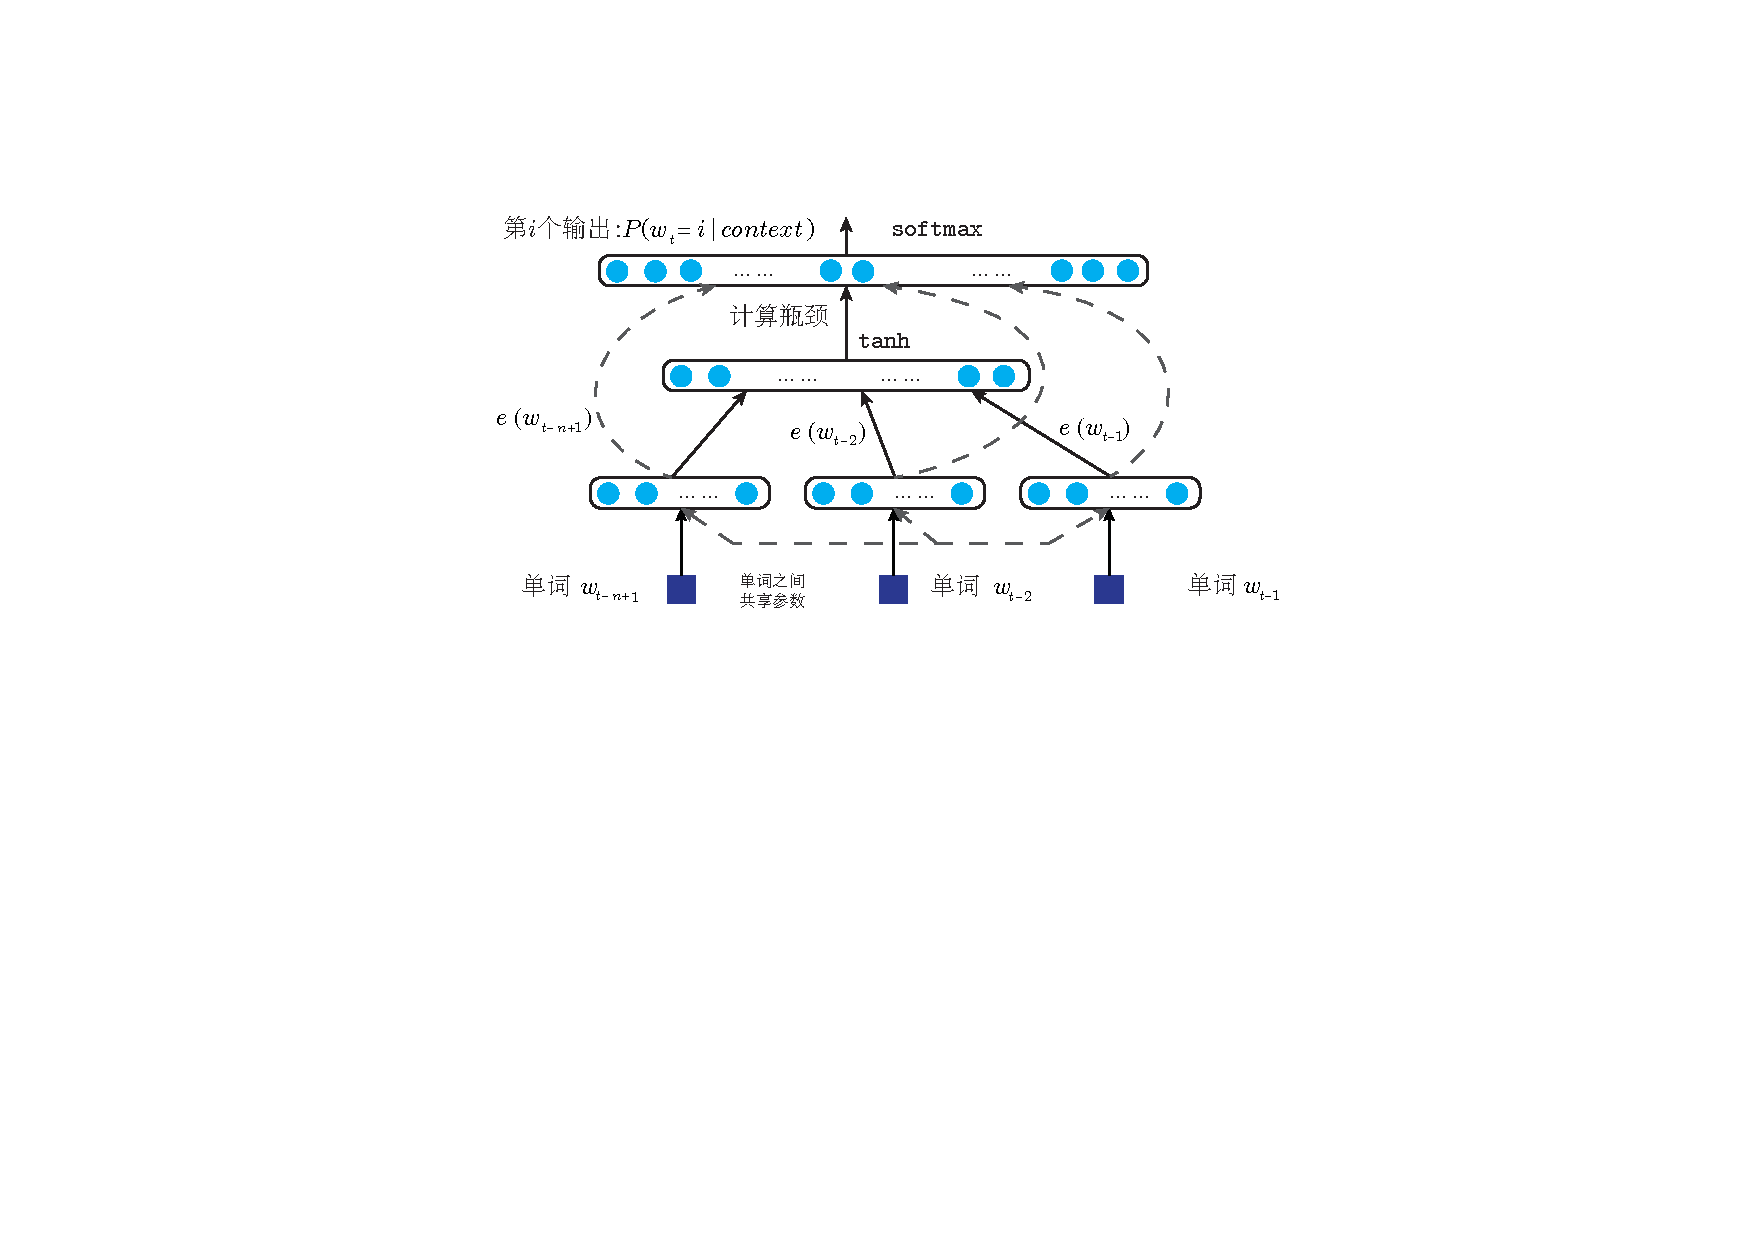
\includegraphics[width=.85\linewidth]{./figures/nplm.pdf}
  \caption{前馈神经网络语言模型}\label{fig:nplm}
\end{figure}

图~\ref{fig:nplm} 给出一个典型的采用三层前馈神经网络结构 NPLM 语言模型。其中输入层用于表征前$n$个单词的高维分布;隐藏层,表征单词的上下文信息,最后一层是输出预测层,预测下一时刻的可能出现的单词概率分布。为了解决数据稀疏问题,Bengio~等人提出拼接(Concatenation)各词的词向量作为输入,如下所示:
\begin{equation}\label{equ:we}
  x = [e(w_{i-(n-1)}), \cdots , e(w_{i-2}), e{(w_{i-1})}]
\end{equation}
模型的隐藏层$h$ 和输出层$y$可以依照下面的公式计算获得:
\begin{equation}\label{equ:nplm}
\setlength{\abovedisplayskip}{6pt}
\setlength{\belowdisplayskip}{6pt}
\begin{split}
h =& \tanh(Hx+b) \\
y =&Wx + Uh +b'
\end{split}
\end{equation}
其中参数矩阵~$H,W,U$~指代层与层之间的权重\upcite{赵林2007一种新的基于结构的神经网络规则抽取方法},参数向量~$b,b'$~均为模型中的偏置项(Bias)。如果存在$W$,那么模型能直接学习一个线性模型,需要训练的时间减少;如果不存在$W$,模型学习到非线性的网络模型,具有更好的泛化性(Generalization)。因此在后续工作中,很少有使用输入层到输出层直连边的工作,下文我们也直接忽略这一种直连的操作。假设不考虑$W$ 矩阵,整个模型计算量最大的运算,就是从隐藏层到输出层的矩阵运算$Uh$,后续的模型均有对这一矩阵乘法计算做优化。

\subsection{对数双线性语言模型}
2007 年,Mnih 和 Hinton 在神经网络语言模型(NNLM)的基础上提出了对数双线性语言模型(Log-Bilinear Language Model, LBL)~\upcite{DBLP:conf/icml/MnihH07}。LBL~模型与~NNLM~模型的区别正如它们的名字所示,其中~LBL~的模型结构是一个对数双线性结构;~NNLM~的结构不包含双线性结构,仅仅是简单的前馈网络。具体来讲,LBL 模型的代价函数为:
\begin{equation}
\setlength{\abovedisplayskip}{6pt}
\setlength{\belowdisplayskip}{6pt}
\label{equ:lbl}
\begin{split}
   &\hat r=\sum_{i=1}^{n-1}{U_i e({w_i})}, \\
   &p(w_n=w|w_{1:n-1})=\frac{\exp(\hat r^\top e(w))}{\sum_j{\exp(\hat r^\top e(w_j))}}
\end{split}
\end{equation}
其中 $\hat r$ 代表了语言模型的上下文信息,$U_i$ 指代的是对应单词的权重向量。然后基于上下文信息表示 $\hat r$ 和下一个单词的目标词汇表中所有单词 $e(w),w\in \mathcal{V}$ 的表示之间的相似度来计算下一个单词的可能的概率分布。

公式~(\ref{equ:lbl})~所描述LBL模型的代价函数与公式~(\ref{equ:nplm})~所描述~NNLM~模型的代价函数的主要区别有:1) LBL 模型中,没有非线性的激活函数$\tanh$,而由于NNLM 是非线性的神经网络结构,激活函数必不可少;2) LBL 模型中,只有一份词向量$e$,也就是说,无论一个词是作为上下文,还是作为目标词,使用的是同一份词向量。其中第二点(只有一份词向量),只在原版的LBL 模型中存在,后续的改进工作均不包含这一特点。

后来,Mnih~等人以~LBL~模型为基础,并对其所存在缺点做了一系列改进工作。其中最重要的模型有两个:逆向量语言模型(inverse vector LBL,ivLBL)~\upcite{DBLP:conf/nips/MnihK13}和层次对数双线性语言模型(Hierarchical LBL,HLBL)~\upcite{DBLP:conf/icml/MnihT12}。

\subsection{循环神经网络语言模型}
对于循环神经网络来说,它能直接对序列概率~$p(w_t | w_1,w_2,\cdots,w_{t-1})$~进行建模,而不使用公式~(\ref{equ:approx})~对其进行简化~\upcite{mikolov2012statistical,DBLP:conf/interspeech/MikolovKBCK10} 。RNNLM 模型结构如图~\ref{fig:rnnlm}~所示,它的核心方法在于其隐藏层的计算公式:
\begin{equation}
\setlength{\abovedisplayskip}{6pt}
\setlength{\belowdisplayskip}{6pt}
\label{equ:rnn}
  h_t \leftarrow  \phi(e(w_t) + U h_{t-1} +b),
\end{equation}
其中 $\phi$ 为非线性激活函数。在上述公式中,$h_t$ 表示文本中第 $t$ 个词 $w_t$ 所对应的隐藏层,该隐藏层由词向量 $e(w_t)$ 以及上一个步的隐藏层输出 $h_{t -1}$ 计算得到。隐藏层的初始状态为$h_0$,随着模型逐个读入单词:$w_1,w_2,\cdots$, 隐藏层根据公式~(\ref{equ:rnn})~被计算出来并被输出:$h_1,h_2,\cdots$ 。通过这种自身迭代更新方式,囊括了此单词前所有上文的信息,相比NPLM模型,RNNLM 理论上能学习到更丰富、更长距离的知识,也有更大的潜力达到更好的效果。最后,RNNLM 模型的输出层与NPLM 模型的输出层都采用softmax算法,两者是一致的。

\begin{figure}
  \centering
  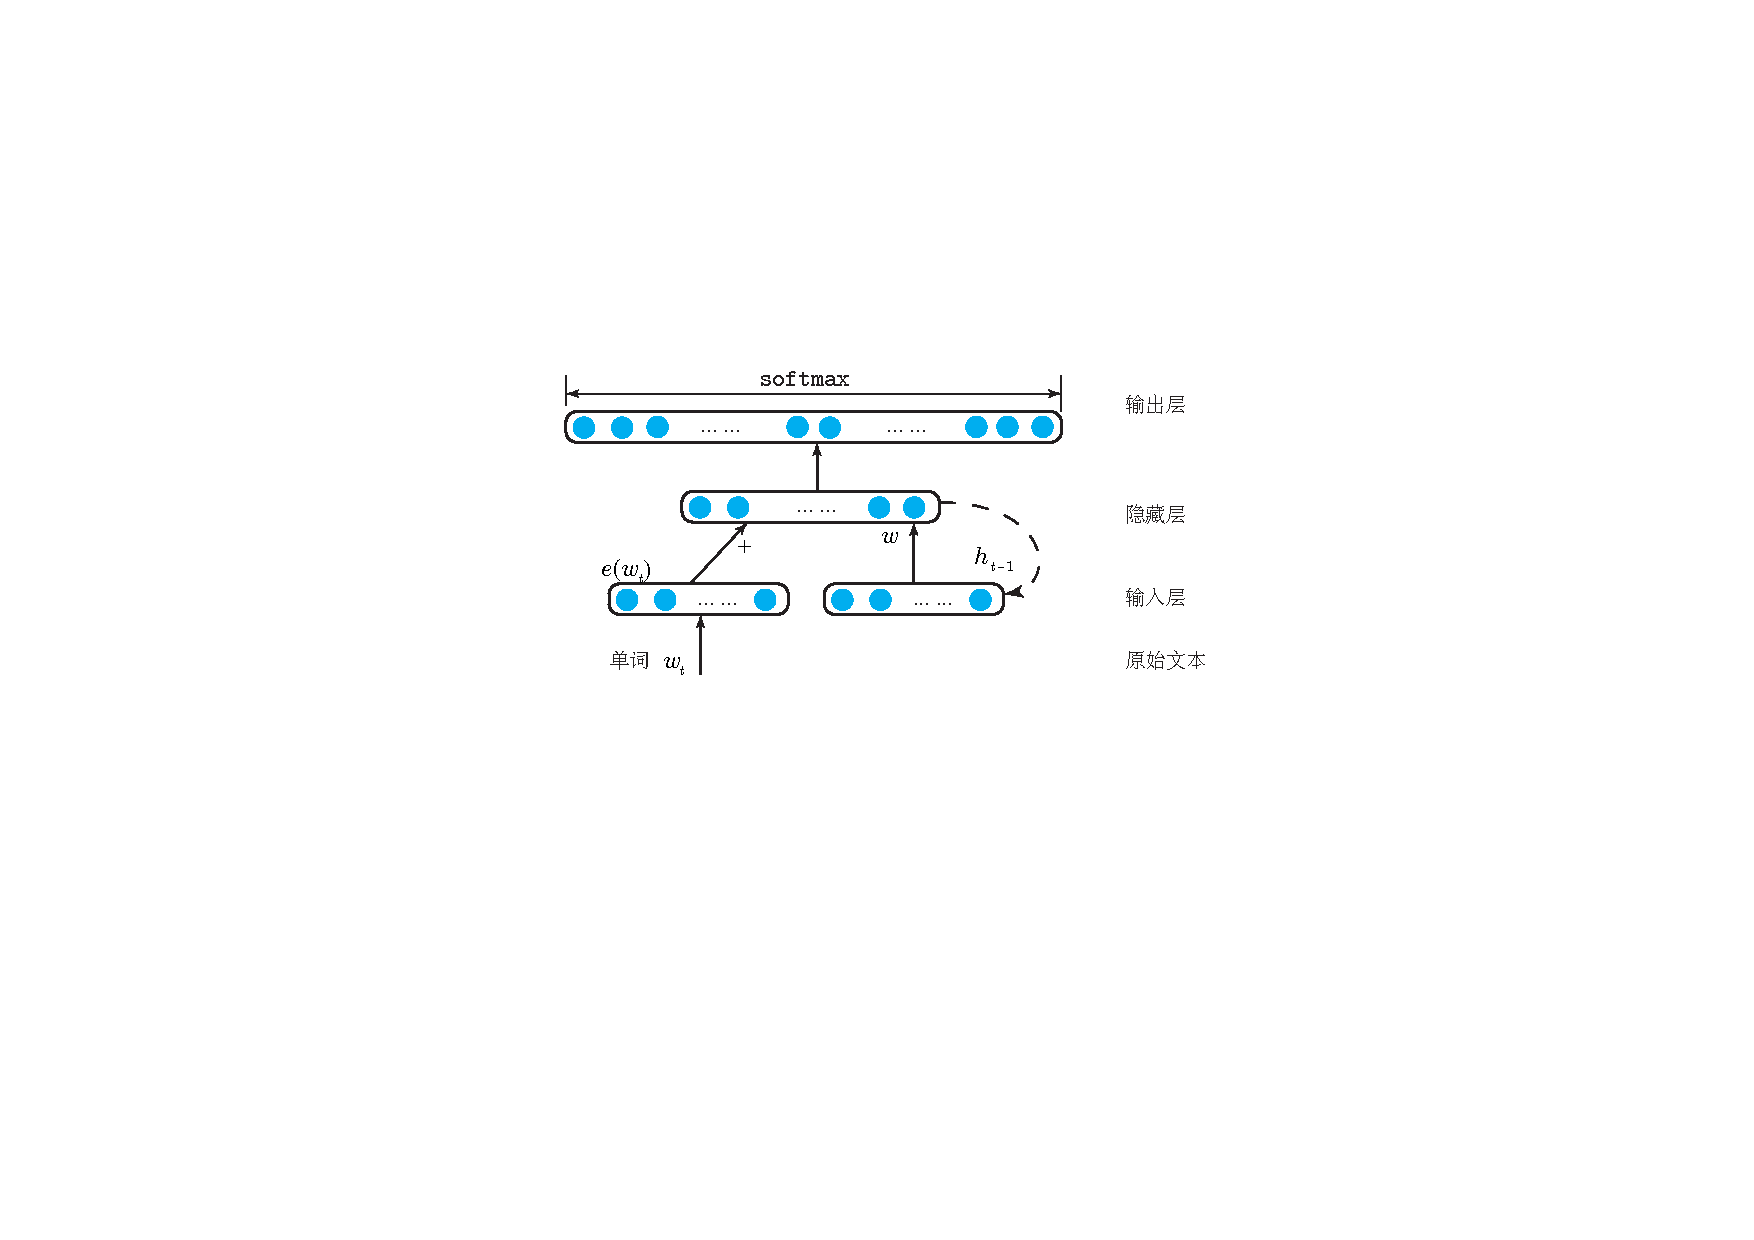
\includegraphics[width=.8\linewidth]{./figures/rnnlm.pdf}
  \caption{循环神经网络语言模型结构图}\label{fig:rnnlm}
\end{figure}


除了介绍的两种经典的建模方法,最近研究者提出可以使用带有门限机制(Gating)的RNN来防止模型的长距离依赖问题,例如长短记忆网络(Long Short-Term Memory, LSTM), 门限记忆节点(Gated Recurrent Unit, GRU)和其他网络。


\section{论文研究内容}
在历史文献当中,源词和目标词分别被称为模型的输入和输出。源词通常可以用分布式表示(Distributed Representation)来表示,称为输入词嵌入(Word Embedding),可以使用基于外部语料库的连续词袋模型(CBoW)或跳跃单词模型(Skipgram)模型来训练。而这两个模型来源于语言模型任务,并且为了在特征空间中产生可能的嵌入分布而被大大简化。另外,输出字通常表示为字索引(Indexing)或~$1-K$~编码,并且可以与softmax概率函数直接关联。

语言模型的大词表问题是目前理论应用到实际过程中必须要克服的问题,我们当然可以通过配置高性能服务器来暂时延缓该问题的后果。但是一旦应用到大数据集上,即使是目前最好的中央处理器(CPU)或者图形处理器通用计算(GPGPU),仍然需要一个多月时间才能训练完善。因此,在保证原有模型的准确率和精度的前提下,如何提高模型的训练速度是我们主要讨论和研究的内容。为此我们讨论了两个不同的内容:上下文信息建模效率和精度对比和大词表问题的优化和研究。

针对上下文信息建模手段,目前主要采用的方案有以下几种:一种是采用子词(Subword-level)或者字符级别的词(Character-level)来直接缩小词表大小;一种是通过采样技术(Sampling-based Approximation)来减少必要的训练时间;一种是通过基于分类的多元分类(class-based Hierarchical Softmax, cHSM)来加速模型和采用基于树模型的多层二元分类模型(tree-based Hierarchical Softmax, tHSM)。同时,我们还需要针对CPU 和GPGPU设备分别进行探讨。因为传统的线性运算模型在流行的GPGPU并行运算方案中并不适用,所有需要结合不同的运算设备分别讨论可行的方案。

在本节中,我们将这个目标词表示扩展到一个分层的形式,使它们适配基于类和基于树的分层概率计算。首先,我们提出了一个在分层结构上建模参数的字编码方案。因此,考虑到~GPGPU~上的并行吞吐性能,我们推导出紧凑的代价函数及其梯度。同时,类或树上的单词分布对其性能有很大的影响,应该在训练阶段之前定义,这些动态交换算法在训练过程中改变了单词群或子树结构在这个研究中。我们采用了几个分层聚类和词汇分割策略,用统计,句法和语义知识来初始化其结构,以达到一个稳定和可以预期的性能。而且,在推理过程中,不同于传统的softmax情况,得到最好的候选者自然是可行的,层次推理不能直接用 softmax 方法来实现。我们讨论基于树和基于类的搜索策略的两种不同的推理情况:1)打分:输出给定序列的概率;2)排序   :在给定的上下文中获取得分最高的一个候选单词。
\section{论文的组织结构}
\textbf{第一章:}``绪论'',主要介绍了本论文的研究背景和意义,另外简要说明了语言模型的发展历史以及本文的主要工作,并对本文的组织架构进行了说明。

\textbf{第二章:}``相关技术介绍'',对历史上的各个学术流派在语言模型的任务上相关工作进行了介绍。

\textbf{第三章:}``并行树状概率模型'',介绍了基于二叉树的层次概率模型,并比较了传统树状模型的差一点。同时还研究了在推理测试阶段,二叉树层次概率模型能应用的策略,以保证实际测试结果性能和效率。


\textbf{第四章:}``并行分类层次概率模型'',介绍基于分类的层次概率模型,并分析了词表非均匀划分所产生的后果,进而探讨了类别不均匀问题所带来的影响以及相关解决策略。最后探讨了在测试阶段,语言模型的任务需求和分类层次概率模型相应的解决算法。

\textbf{第五章:}``语言模型实验及实验结果分析'',实证研究了本论文提出的并行层次概率模型的实际效果,并和其他算法在各个指标维度上进行了比较和分析。

最后结论部分,总结了全论文的贡献和工作,并提出了未来的工作方向,同时撰写了结束语。




\chapter{相关技术介绍}
\section{引言}
在自然语言处理研究领域中,基于神经网络的分布式表示(Distributional Representation)一般统称为词向量(Word Vector)、词嵌入(Word Embedding)或者分布式表示(Distributed Representation)~\upcite{DBLP:conf/nips/MikolovSCCD13}。神经网络词向量表示技术,是通过神经网络技术对:1)单词的语境,即上下文(Context);2)以及上下文与下一步的目标单词之间的关系(Next-Utterance Prediction),这两个主要的部分进行建模。
由于神经网络结构或各种组合较为灵活,这类方法的最大优势在于可以表示复杂的上下文语义(Complex Context)。历史上的方法主要是基于单词共现矩阵(Co-occurrence Matrix)的分布表示方法,最常用的上下文仅仅是利用了单词的顺序信息。单词的语义向量是通过给这个单词共现矩阵进行矩阵分解,例如奇异值分解(Singular Value Decomposition,SVD),潜在语义分析(Latent Semantic Analysis,LSA),也可以写成潜在语义索引(Latent Semantic Indexing,LSI)分解算法。其中对于SVD分解算法,第一个分解获得的矩阵就是我们模型输出的单词的词向量矩阵。然而,如果使用包含词序信息的~N-gram~作为上下文,当~$N$~增加时,N-gram 的所需要存储的单词序列总数会呈指数级增长,此时会遇到维数灾难问题(Curse of Dimensionality)\footnote{https://en.wikipedia.org/wiki/Curse\_of\_dimensionality}。这一瓶颈深深限制了~N-gram~模型的实际应用。而用神经网络替代表示~N-gram~的单词概率分布时,可以通过一些组合方式对~N~个词进行组合,其优点显而易见:神经网络语言模型所需要的参数数量仅以线性速度增长。有了这一优势,神经网络模型可以对更复杂的上下文进行建模,在从训练后的模型提取出来的词向量中包含更丰富的语义信息。

到目前为止,在语言模型的研究领域中,所应用到的神经网络模型主要包括: 传统前向传递神经网络(Feed Forward Neural Network, FFNN)、循环神经网络(Recurrent Neural Network, RNN)三种基本的建模方案。当然基于这些基本组件,我们还可以构造更复杂的模型结构,但是我们无法保证复杂模型一定在效率和精确度上优于简洁的模型结构。复杂的模型可以表征更复杂的本文语义信息,例如句子的依存关系结构或者句子的句法分析树结构,但是这样的效果不一定能保证模型的泛化性能(Generalization)会很好,因为日常聊天文本的语序是混乱的,很难找到学者良好定义的句子关系,所以也无法让模型从混乱的文本分布中学习到有效的句子结构,以提升模型的精度。最好的模型,显然是假设越弱越合适,因为针对复杂的网络文本数据,我们模型训练所需要的要求越弱,模型越容易收敛并获得我们想要的结果。模型假设越强,模型所需要的数据质量越高,实际稳定性就会降低,产生得不偿失的后果。

语言模型的历史发展
除此以外,针对在本论文所讨论的语言模型的大规模应用过程中所遇到的大词表问题,目前现有的主要解决方法主要可以分为以下三种种策略:单词拆分算法(Vocabulary Truncation)、采样估计模型(Sampling-based Approximation)和层次分解模型(Vocabulary Factorisation),我们会在接下来的章节陆续介绍。其中本论文重点是研究基于类别的多元分类模型(class-based hierarchical softmax, cHSM)和基于二叉树的二元分类模型(class-based hierarchical softmax,tHSM),这两种算法我们分别在下一章更详细讨论和介绍。

\section{语言模型}
在这一节中,我们将首先从语言模型提出的实际任务的形式化定义开始,以阐述语言模型的训练目标和实际应用场景~\upcite{DBLP:journals/tnn/ChienK16}。一个好的语言模型应当考虑对文本的两种特征进行建模:语法特征(Syntactics)和语义特征(Semantics)。为了保证语法的正确性,我们往往只需要考虑生成的单词的前面的上下文(Previous Context),这也就意味着语法特性往往只对局部特征(Local Representation)进行建模。而语义特征的一致性则复杂了许多,它意味着我们需要考虑更大、更完善的上下文信息乃至整个文档语料,来获取正确的全局语义(Global Context)而不仅仅是局部语义信息(Local Context)。


具体地来说,给定一个包含$T$个单词的序列:$w_1,w_2,\cdots,w_T$,这个序列的对数概率(Log-probability),即描述该序列作为一个合理且合法的句子的流畅性(Fluency)概率和出现该单词组合的句子的可能性( Likelihood),可以使用马尔可夫链规则分解成一系列的条件概率的联合分布:
\begin{equation}
\label{laguage_model}
 \log p(w_1,\cdots, w_T ) = \sum_{t=1}^T \log p(w_t | w_{1:t-1}),
\end{equation}
其中前 $t-1$个单词在本论文中一律记作$w_ {1:t-1}$。进而,条件概率~$p(w_t | w_ {1:t-1})$表示给定其前面上下文$w_ {1:t-1} $作为预测的下一个单词的条件概率分布(Conditional Probability)。最早的传统方法可以由前馈网络来建模这个上下文信息, 同时用多标签概率函数(Multi-class Classification)来表示下一个单词的概率分布计算公式~\upcite{DBLP:journals/jmlr/BengioDVJ03}。 在训练的过程中,整个模型以最小化每个单位预测步骤里面的交叉熵损失(Cross Entropy Loss):
\begin{equation}\label{equ:losses}
  \ell=\sum_{t=1}^{T}\ell_t=\sum_{t=1}^{T}\log p(w_t | w_{1:t-1})
\end{equation}
其中文本或者句子的交叉熵的代价函数$\ell$ 的实际定义为:是当编码方案不一定完美时(由于对概率分布的估计不一定正确),平均编码长度的是多少。这里的编码长度就是指的是如何用01字节对所有的单词进行最短的编码,保证单词之间两两不互相冲突。它是由$ \texttt{KL}$散度(Kullback–Leibler Divergence),也叫做相对熵(Relative Entropy),推导而获得的。需要注意的是,$  \texttt{KL}   $散度的计算公式是:
\begin{equation}\label{equ:losses}
  \texttt{KL}(p||q)=-\sum_{t=1}^{T}p(x)\log q(x) - (\sum_{t=1}^{T}p(x)\log p(x))
\end{equation}
其中$p(x)$ 指的是数据的真实概率分布,$q(x)$ 是由数据计算得到的概率分布。需要注意的是,由于$p(x)$ 和$q(x)$ 在公式中的地位不是相等的,所以$   \texttt{KL} (p\parallel q)\not\equiv  \texttt{KL}  (q\parallel p)$。对于特定的训练数据集,第二项的计算值是常数,由此可知其导数是0,不会对参数更新产生任何影响,所以通常情况下,我们采用交叉熵函数作为模型的代价函数,但其实我们希望模型优化的目标是使得模型的分布拟合实际的分布。
\subsection{语言模型的应用}
语言模型的作用主要分为以下三种:1) 为句子打分(Sentence Scoring)。给定一个未知的单词序列,我们需要计算其作为一个句子的流畅性和出现的可能性;2) 挑选最佳的候选词(Next Utterance Prediction)。给定上下文,选择概率最高的单词。上下文的形式可能是:前面的句子给定,选择下一个最佳单词;前面和后面的句子给出,选择中间最适配的单词。3) 训练词向量(Pretrained Word Embedding)。语言模型的输入,在经过大规模数据集训练之后,可以作为词向量输出,从而为其他文本任务提供有效的特征。

\subsection{长距离依赖}

不同于前馈神经网络语言模型,循环神经网络语言模型使用隐藏层状态来记录单词的顺序性信息,能够捕捉句子中的长距离依赖(Long-term Depnendency)。这里的长距离依赖主要指下面的两方面。

一方面,在自然语言中,往往在句式中相隔较远的两个词却具备一定的语法与语义关联。譬如:
\begin{verbatim}
He doesn't have very much confidence in himself
She doesn't have very much confidence in herself
\end{verbatim}
这两句话中的``(He, himself)'' 与 ``(She, herself)'' 这两个词对,尽管句子中间的词可能会发生变化,但是这两种词对中两个词之间的关联却是固定的。这种依赖也不仅仅出现在英语中,在汉语、俄罗斯语中也都存在有大量此类型的词对组合;

而另一种长期依赖就是指选择限制(Selectional Preferences)。简而言之,选择限制主要基于已知的某人会去做某事这样的信息。譬如我要用叉子吃沙拉与我要和我的朋友一起吃沙拉这两句话中,叉子指代的是某种工具,而我的朋友则是伴侣的意思。如果有人说我要用双肩背包来吃沙拉就觉得很奇怪了,双肩背包并不是工具也不是伴侣。如果我们破坏了这种选择限制就会生成大量的无意义句子。

\begin{figure}[!ht]
  \centering
  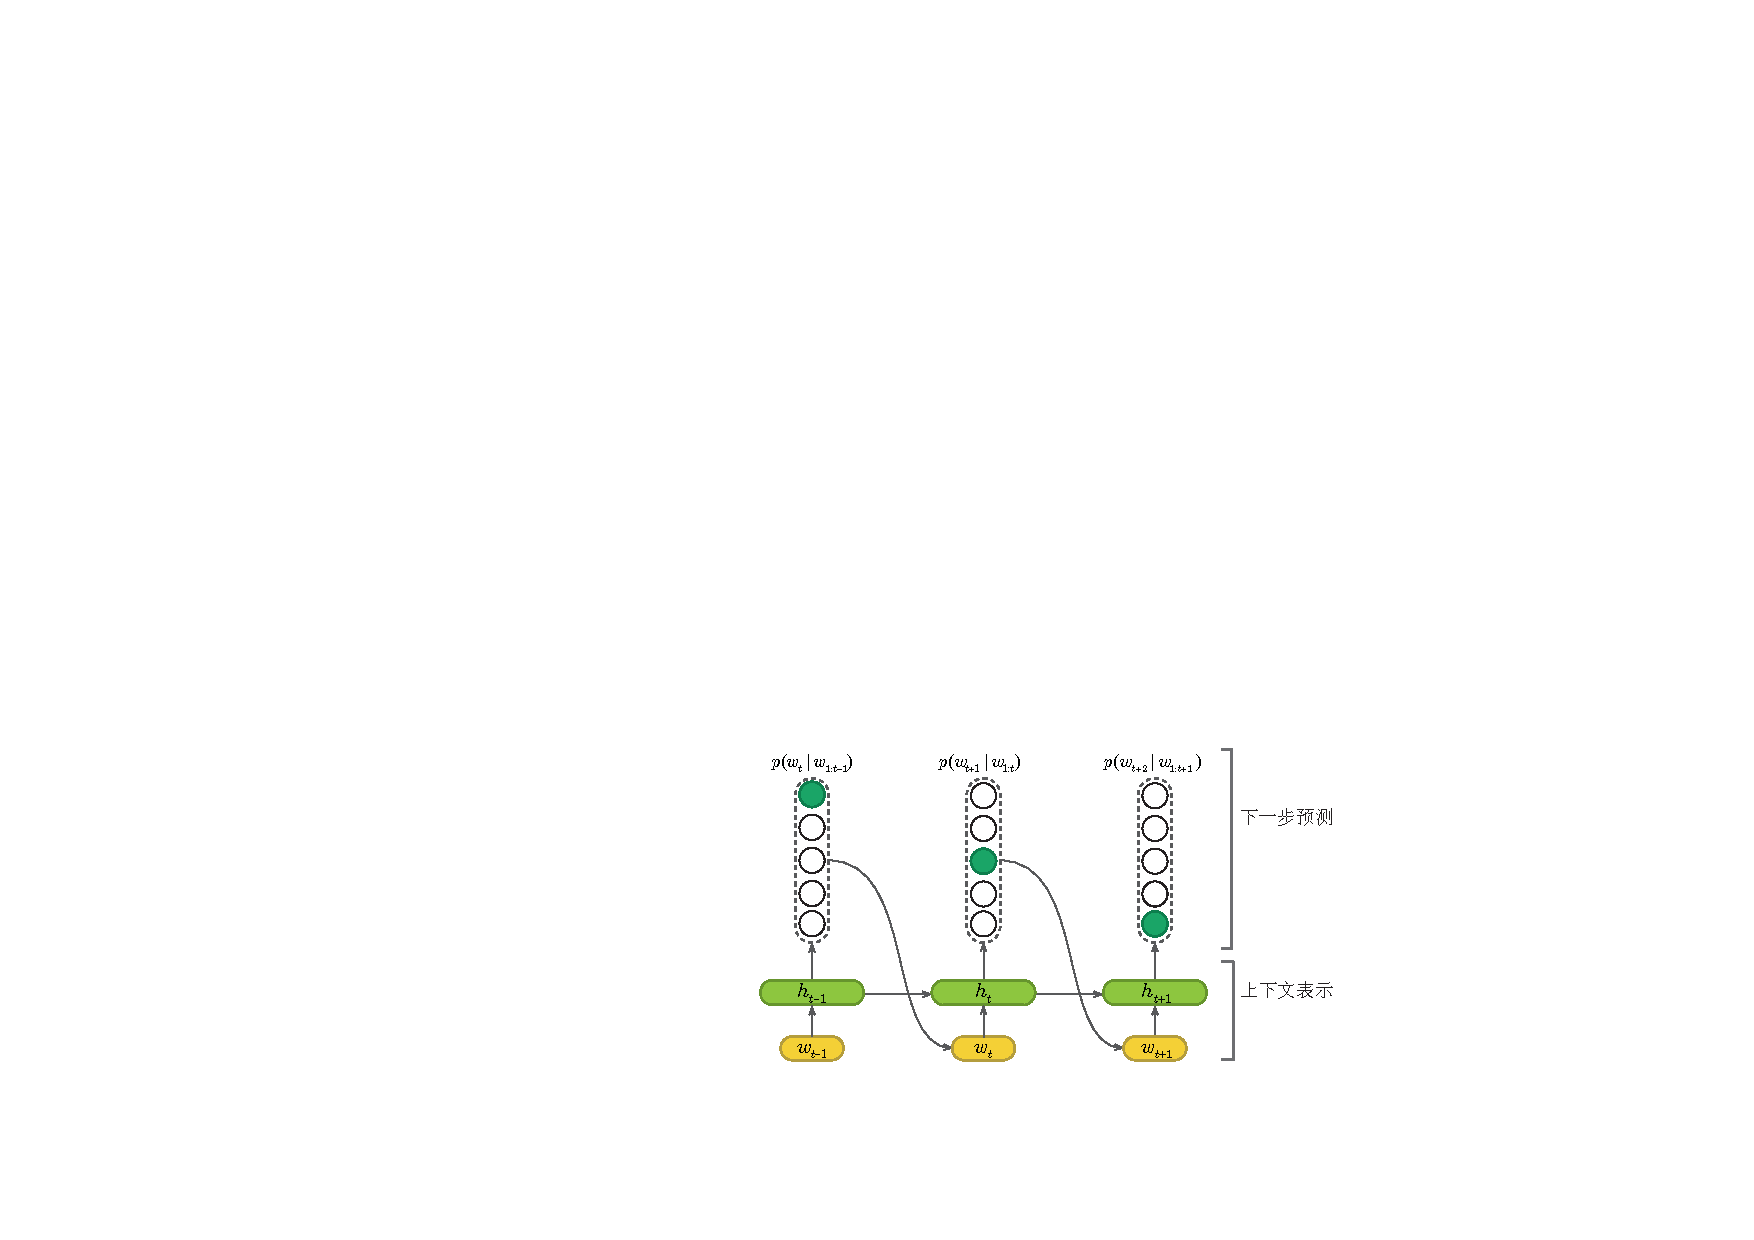
\includegraphics[width=1\columnwidth]{./figures/lm.pdf}
  \caption{循环神经网络语言模型图例}
  \label{fig:lm}
\end{figure}

\subsection{循环神经网络}
所以,考虑到上述长距离依赖问题,本实验采用的基准模型就是基于循环神经网络的语言模型。最近,利用序列的时间序列信息的循环神经网络已经非常流行,如图~\ref{fig:lm}~所示。 为了清楚起见,由于在当前时间步 $ t $的输出$ w_ {t + 1} $正好是下一个时间步的输入$ w_ {t + 1} $,所以没有输出的自动关联连接(Auto-associative Connection)的前一次步骤$ t $回到下一个时间步骤$ t + 1 $中的循环神经网络。每个句子都需要用开始词(即,$ \langle s \rangle $)和结束词(即$ \langle / s \rangle $)标记进行封装。 在预测下一个单词 $ w_ {t + 1} $ 之前,从最后一个隐藏状态$ h_ {t-1} $和当前字$ w_t $接收到循环网络单元的输入。

从形式上讲,循环神经网络是一个参数化的非线性函数$ \mathtt{RNN} $,循环地将一系列向量映射到一系列隐藏状态。 将$ \mathtt{RNN} $应用于任何这样的序列,在每个时间步骤$ t $产生隐藏状态$ h_t $,如下所示:
\begin{equation}
  h_t \leftarrow  \mathtt{RNN}(W\theta^w_t + U h_{t-1} +c),
\end{equation}
其中$ W,U $是模型参数的集合,而$ U $是随时间共享的,向量$ \theta^w_t$ 对应于源词的嵌入$ w_t $。

自Elman提出基本循环网络模型~\upcite{DBLP:journals/cogsci/Elman90}~以来,已经有许多扩展模型提出了克服长距离依赖,梯度消失(Gradient Vanishing)和梯度爆炸(Gradient Exploding)等问题, 如长期短期记忆网络(LSTM)~\upcite{7508408},门限记忆单元(GRU)~\upcite{DBLP:conf/nips/ChungKDGCB15}和近似递归神经网络(Quasi-RNNs)\upcite{DBLP:journals/corr/BradburyMXS16}。

\begin{figure}[!ht]
  \centering
  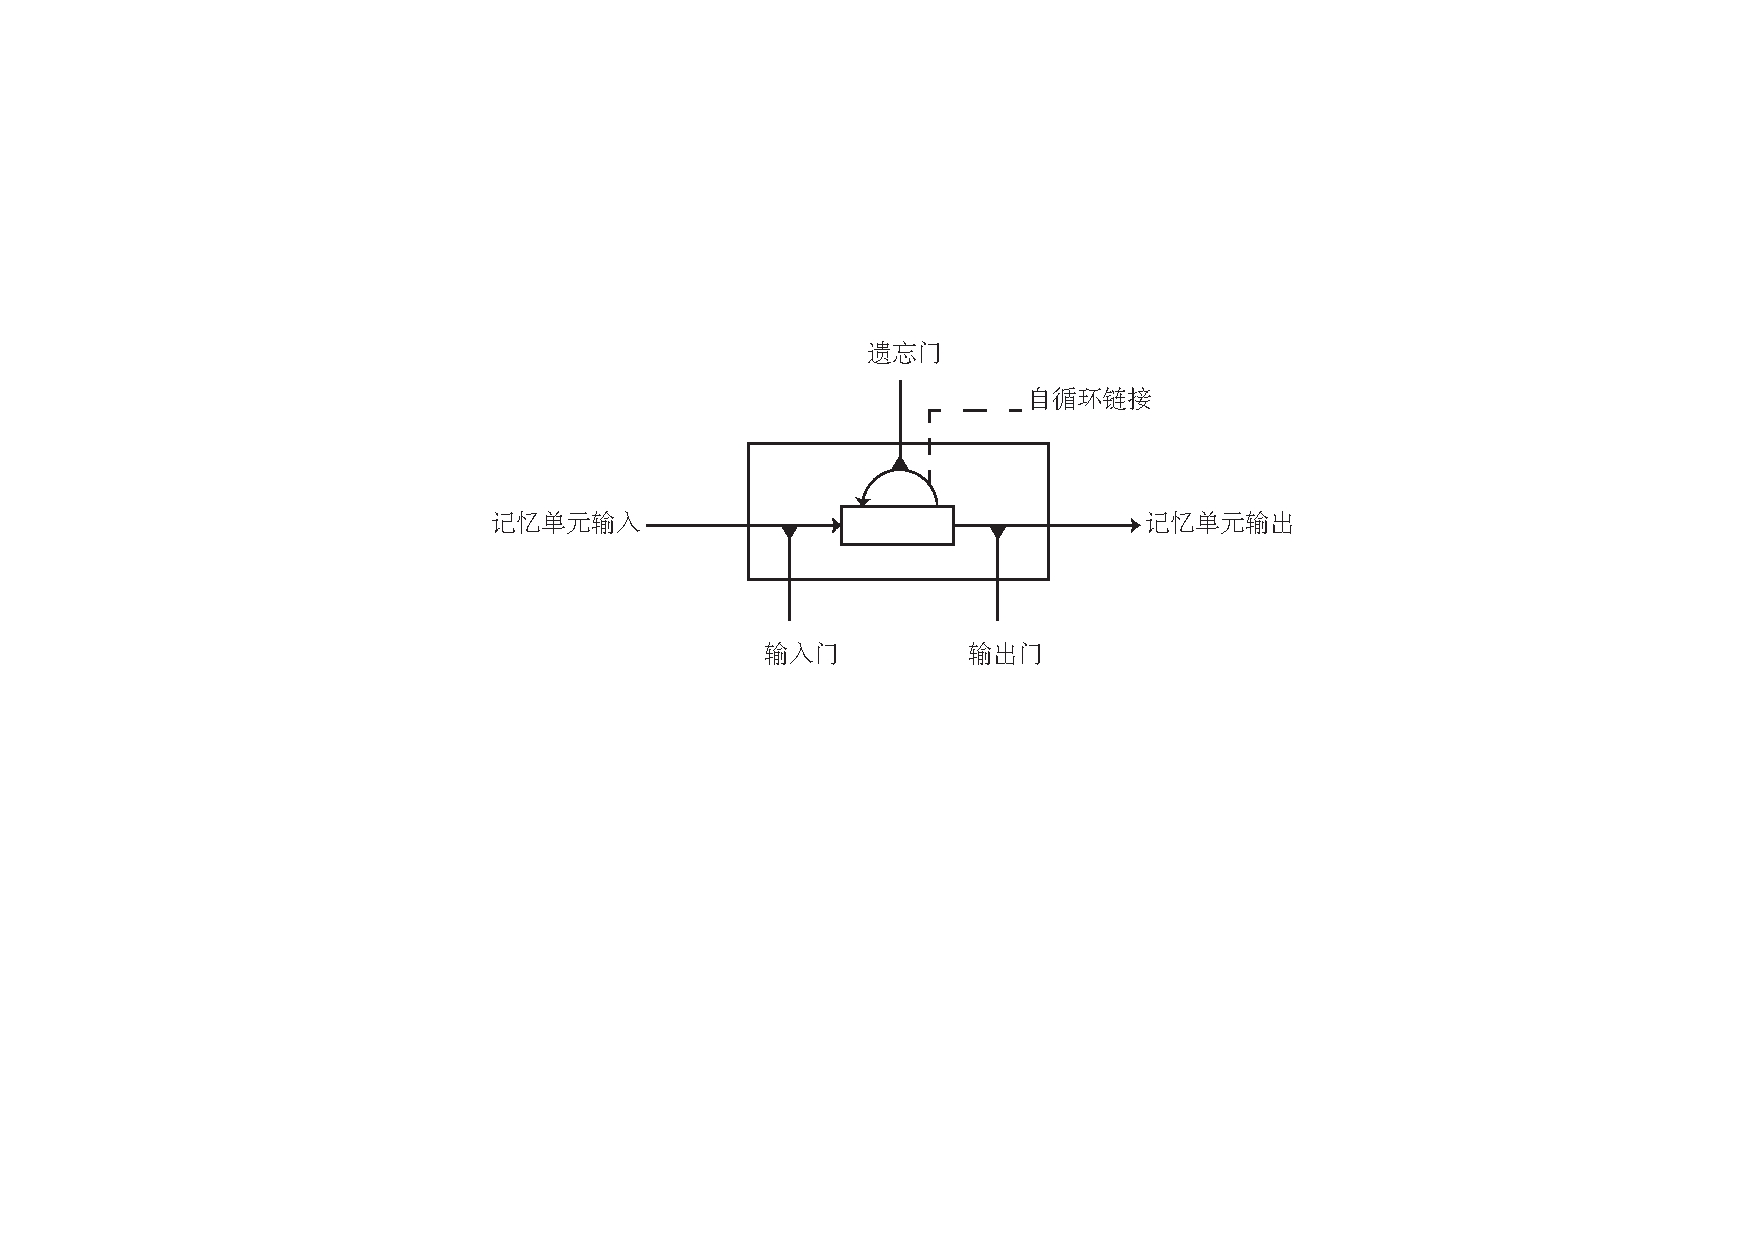
\includegraphics[width=0.7\linewidth]{./figures/lstm.pdf}
  \caption{LSTM 模型示意图}\label{fig:lstm}
\end{figure}

{长距离短期记忆网络}。LSTM的计算公式定于如下 \upcite{DBLP:journals/neco/HochreiterS97}:
\begin{itemize}
\item 输入门。控制当前输入 $x_t$ 和前一步输出 $h_{t−1}$ 进入新的 cell 的信息量:$i_t=\sigma(W^i x_t+U^i h_{t-1}+b^i)$
\item  遗忘门。决定是否清楚或者保持单一部分的状态$f_t=\sigma(W^f x_t+U^f h_{t-1}+b^f)$
\item  变换输出和前一状态到最新状态$g_t=\phi(W^g x_t+U^g h_{t-1}+b^g)$
\item  输出门。计算 cell 的输出$o_t=\sigma(W^o x_t+U^o h^{t-1}+b^o)$
\item  cell 状态更新。步骤:计算下一个时间戳的状态使用经过门处理的前一状态和输入:$s_t=g_t\odot i_t+s_{t-1}\odot f_t$
\item 最终 LSTM 的输出:使用一个对当前状态的 $\tanh$ 变换进行重变换:$h_t=s_t\odot \phi(o_t)$
\end{itemize}
\noindent 其中$\odot$ 代表对应元素相乘(Element-wise Matrix Multiplication), 函数 $\phi(x), \sigma(x)$ 的定义如下:
\begin{equation}\label{equ:tanh}
  \phi(x)=\frac{e^x-e^{-x}}{e^x+e^{-x}},\sigma(x)=\frac{1}{1+e^{-x}}
\end{equation}

{并行计算实现方法}。输入门、遗忘门、输出门和状态更新门矩阵乘法可以并行实现,从而提高LSTM模型的计算效率。因为LSTM的计算模型更容易并行,所以他与GRU的计算时间相差无几,尽管LSTM的模型需要的参数量是GRU模型的1.5倍。
\begin{equation}\label{equ:lstm}
\begin{bmatrix} i^t\\ f^t\\g^t\\o^t \end{bmatrix} =\begin{bmatrix}\sigma\\ \sigma\\\phi\\\sigma\end{bmatrix}\times W\times[x_t,h_{t-1}]
\end{equation}
其中 $W$ 指的是四个小矩阵互相层叠起来 $[W^i,W^f,W^g,W^o]$。




{门限记忆单元。} GRU 可以看成是 LSTM 的变种,GRU 把 LSTM中的 遗忘门和输入门用更新门来替代。 把 cell state 和隐状态 $h_t$ 进行合并,在计算当前时刻新信息的方法和 LSTM 有所不同。 下图是GRU更新 $h_t$ 的过程\upcite{DBLP:journals/corr/Pezeshki15}, 具体定义如下:
\begin{figure}[!h]
  \centering
  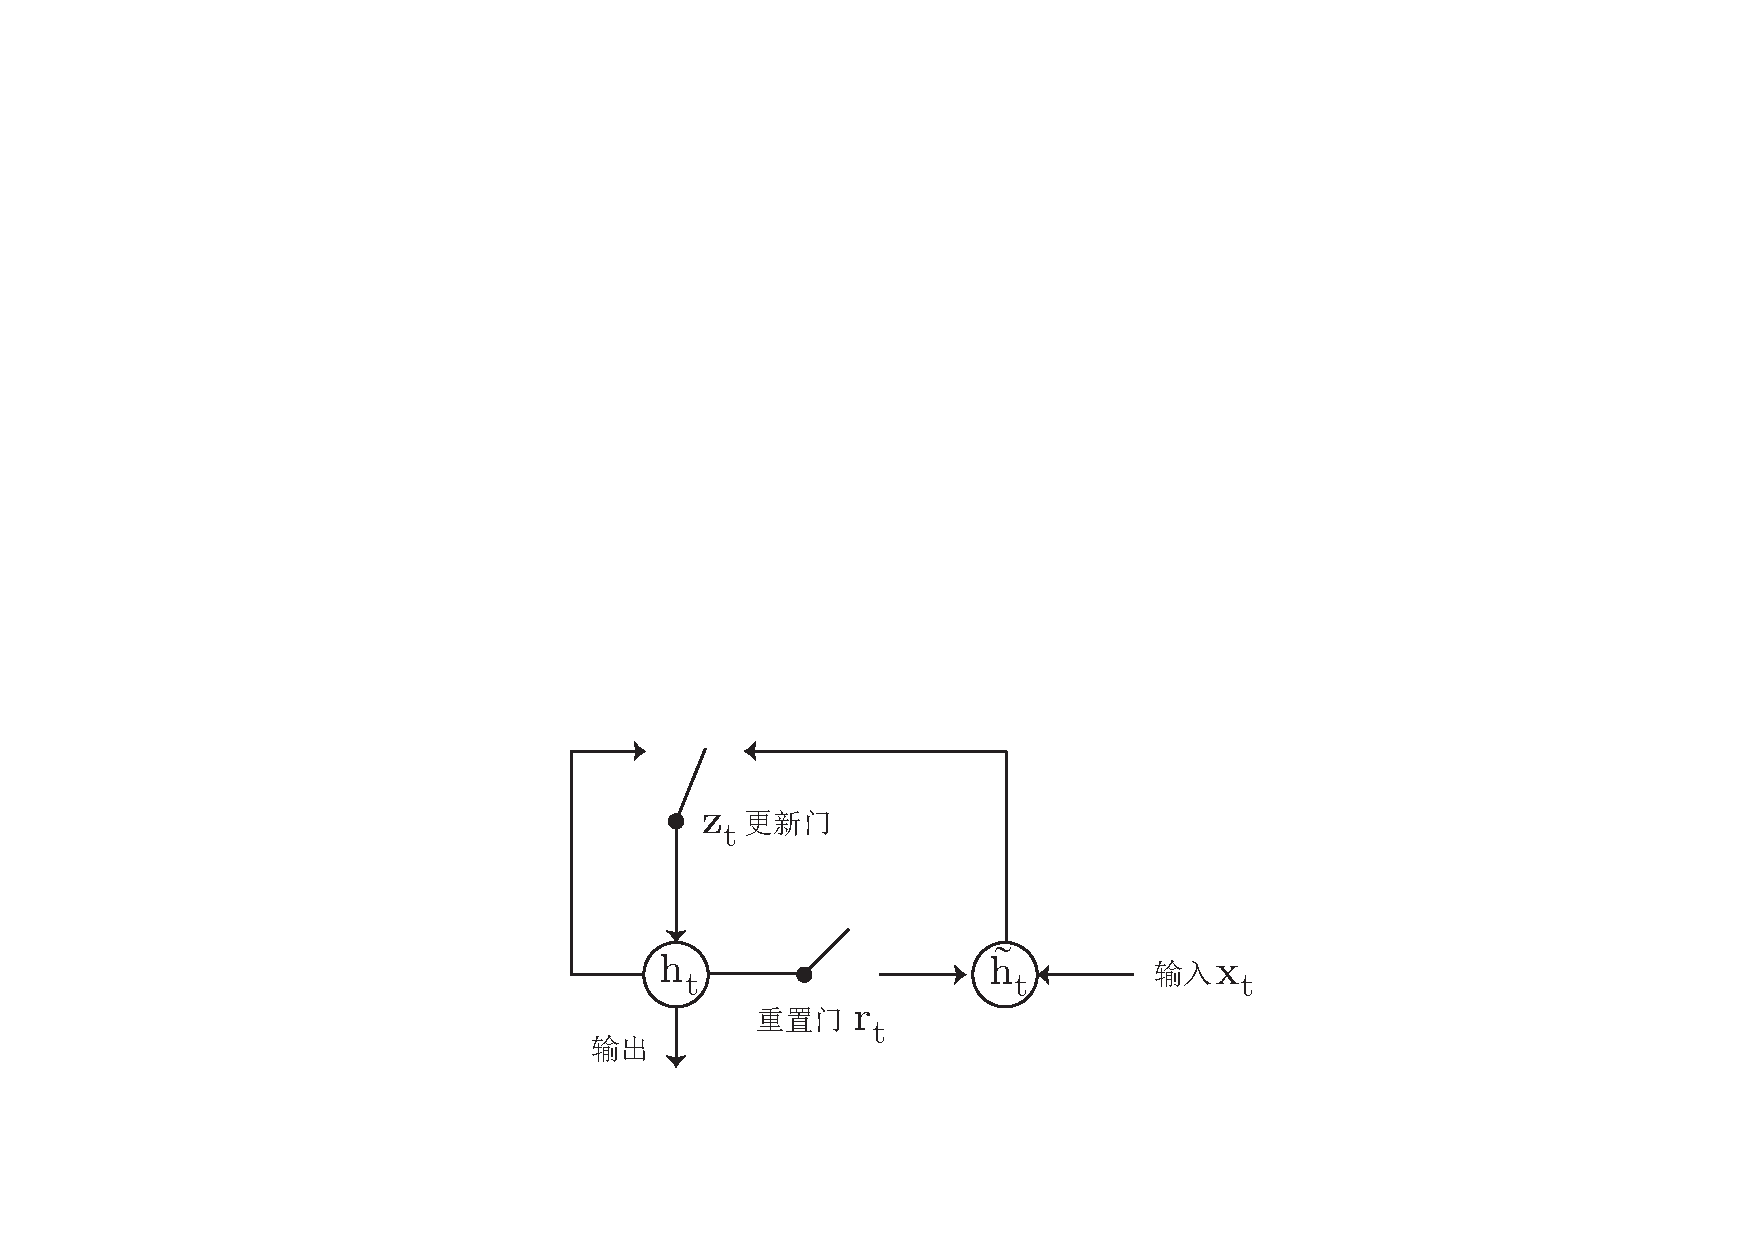
\includegraphics[width=0.45\linewidth]{./figures/gru.png}
  \caption{GRU模型示意图}\label{fig:gru}
\end{figure}

\begin{itemize}
\item 更新门 $z_t$。定义保存多少以前的信息: $z_t = \sigma ( W^z x_t+ U^z h_{t-1}  )$

\item 重置门 $r_t$。 决定保留多少输入信息: $r_t = \sigma(W^r x_t  + U^r h_{t-1}  )$

\item 节点内部更新值$\tilde h_t $。 其次是计算候选隐藏层(candidate hidden layer) $\tilde h_t$,这个候选隐藏层 和LSTM中的$\tilde c_t$是类似,可以看成是当前时刻的新信息,其中$r_t$用来控制需要 保留多少之前的记忆,如果$r_t$为0,那么$\tilde h_t$只包含当前词的信息:$\tilde h_t  = \tanh (W^h x_t  + U^h(h_{t-1} \odot r_t) )$

\item 隐藏层输出值$h_t$。 最后$z_t$控制需要从前一时刻的隐藏层 $h_{t-1}$ 中遗忘多少信息,需要加入多少当前 时刻的隐藏层信息$\tilde h_t$,最后得到$h_t$,直接得到最后输出的隐藏层信息, 这里与LSTM的区别是GRU中没有 输出门:$h_t = (1-z_t)\odot \tilde h_t  + z_t \odot h_{t-1}$
\end{itemize}

如果重置门接近0,那么之前的隐藏层信息就会丢弃,允许模型丢弃一些和未来无关 的信息;更新门 控制当前时刻的隐藏层输出$h_t$需要保留多少之前的隐藏层信息, 若$z_t$接近1相当于我们之前把之前的隐藏层信息拷贝到当前时刻,可以学习长距离依赖。 一般来说那些具有短距离依赖的单元重置门比较活跃(如果$r_t$为1,而$z_t$为$0$ 那么相当于变成了一个标准的RNN,能处理短距离依赖),具有长距离依赖的单元更新门比较活跃。



\section{大词表问题}
作为多标签分类(Multi-class Classification)的标准概率归一化方法,对于大词表问题中,\texttt{log-softmax} 函数和相应的梯度(Gradient)可以定义为:
\begin{equation}
\begin{split}
p(w|h)=&\frac{\exp(h^\top v_{w})}{\sum_{w_j\in \mathcal{V}}{\exp(h^\top v_{w_j} )}} \\
\frac{\partial p(w_i|h)}{\partial v_{w_j}}=&p(w_j|h)(\delta_{ij}-p(w_i|h))h^\top\\
\end{split}
\end{equation}
\begin{equation}
\label{eq:softmax}
\begin{split}
\log p(w|h) &= \theta^w h-\log \sum_{u\in \mathcal{V}}{\exp(\theta^u h)}\\
\nabla_{\theta^u}{\log p(w|h)}&= (\delta_{uw}-p(w|h))h
\end{split}
\end{equation}
其中$ h $是隐藏层输出的向量(即上下文表示),$ \theta ^ w $表示单词$ w $的目标单词嵌入~\upcite{duda2012pattern}。 同样对于克罗内克 $\delta$ 函数$ \delta_ {uv} $(Kronecker Function),如果$ u,v $指代的是相同的单词结果是$ 1 $,如果$ u,v $指代的不是相同的单词则是$ 0 $。


如等式~\ref{eq:softmax}~所示,前向概率传播函数$\log p(w|h) $(即第一行方程)和后向梯度优化函数$\nabla_{\theta^u}{\log p(w|h)}$(即第二行的方程)都需要计算目标词汇表中的所有单词,因此在这个部分上花费的时间会随着词表中包含的单词数量的增加而线性增长。对于包含$ \mathcal{| V |} $ 数量的单词来说,总的时间复杂度是$ \mathcal {O}(\mathcal {| H || V |})$,其中$ \mathcal {| H |} $表示隐藏层输出的维度。即使对于采用现代通用计算体系结构的GPGPU来说, 尽管其非常适合于具有高计算并行的矩阵乘法,这种计算负担也是相当高的。因此,采用现代硬件体系结构的训练和推理中,输出字嵌入矩阵的超大尺寸仍然是一个计算瓶颈。而且,目前的设备的显存是有限的,不能任意增大显存大小,所以对词表大小有一个天然的上限。

值得注意的是,\texttt{softmax} 算法的瓶颈不能归因于``for''循环函数(即方程~\ref{eq:softmax}~)中的$ \sum_ {u \in \mathcal {V}} $,尽管它随着词汇量的增长而线性增长,但是矩阵张量的乘法计算的规模较大。因为矩阵计算需要更多的时间来获得结果,但线性求和可以更快地计算完成。所以,相比于``for''循环函数而言,主要的计算时间用于矩阵乘法计算。我们在这里说明的目的是,只有那些避免其他冗余字的计算概率才能达到边际加速比的方法,而那些仍然涉及全局概率规一化的方法,实际上并不能真正改善这个部分的计算占用的时间。

%其中由于分母是正则项,一旦词表扩大,每次迭代更新都需要计算这一项,是主要的问题所在,所以本课题拟在主要解决该问题所导致的计算费时的问题,

因此,在保证计算精度不下降的情况下,我们期望能缓解计算概率归一化项的计算瓶颈并且提高模型的训练速度。 目前主要缓解大词表问题的算法主要分为以下三类: 单词拆分算法(Vocabulary Truncation)、采样估计模型(Sampling-based Approximation)和层次分解模型(Vocabulary Factorisation)。下面我们将一一详述。


\subsection{单词拆分算法}
针对大词表问题的解决方法,最直接最简单的策略就是我们放弃使用大词表,转而保留一个较小的词表来保证训练的内存占用小和计算效率高。那么针对剩余的过多的词表外的单词(Out-Of-Vocabulary,OOV),我们可以使用传统的N-gram语言模型来估算其可能的概率分布。这样做一方面保证神经网络模型可以在有限时间内训练完,同时保证模型的最后的测试结果不会很差~\upcite{DBLP:journals/csl/Schwenk07}。

然而我们需要注意到,当我们的词表继续减少和我们的所有单词种类不断变多的时候,我们会发现训练样本中存在过多的$\langle$unk$\rangle$ 字符,这样使得神经网络的模型训练非常困难,进而导致模型效果变得非常地差,所以这种方案只是一定程度上缓解了大词表问题,但是也是一种有效的尝试方案。

除了上述直接的建模方案外,目前采用的方案是将单词按照字符级别来划分,可以将一个单词按照字符统计规律划分成任意多个子词。其中二元对编码(byte-pair-encoding,BPE)能将一个单词划分成两部分:前缀(Prefix)和后缀(Suffix)~\upcite{DBLP:conf/icassp/Tucker0P94, DBLP:conf/acl/SennrichHB16a,Gage:1994:NAD:177910.177914},如图~\ref{fig:subword} 所示。从该图中我们可以看出,单词被划分成前缀和后缀两部分,其中$+$代表是单词的前缀,同时$\langle /w \rangle$是单词的后缀。由于划分规则是从训练数据中学习到的,我们可以指定需要缩减的词表大小,所以该算法的动态适应性很强,目前主流的机器翻译模型都采用这个方案~\upcite{DBLP:journals/corr/JozefowiczVSSW16}。尽管如此,我们仍然需要看到它这样的解构操作依然带来了一定的损失,因为句子的长度加倍了,对RNN的长距离关系学习能力提出了更高的挑战~\upcite{DBLP:conf/aaai/KimJSR16}。

\begin{figure}[!h]
  \centering
\includegraphics[width=0.6\linewidth]{./figures/subword.pdf}
\caption{词到子词划分样例}\label{fig:subword}
\end{figure}

\subsection{采样估计模型}
目前采用的采样算法(Sampling Algorithm)主要是针对公式~\ref{eq:softmax}~中对所有单词概率规约那一项进行概率估计,其中著名的算法有:重要性采样(Importance Sampling)~\upcite{DBLP:journals/tnn/BengioS08},噪声差分估计(Noise Contrastive Estimation, NCE)~\upcite{DBLP:conf/icml/MnihT12}和Blackout 采样算法~\upcite{DBLP:journals/iclr/JiVSAD15}。第一种算法在Bengio的实验中被证明模型无法收敛~\upcite{DBLP:journals/tnn/BengioS08},因此目前主要使用的后面两种算法。

对于NCE噪声差分估计算法来说,模型需要学习将正确的单词 $w_0$ 与随机生成的单词 $\{w_1\cdots w_k\}$做一个二元分类。 其中 $w_0$ 训练样本中真正的下一个单词, $\{w_1\cdots w_k\}$ 是采用先验分布  $q(w)$产生的随机噪声单词. 正例归一化后的概率和所有负例联合概率的公式可以写成:
\begin{equation}\label{equ:nce}
\begin{split}
  \tilde{p}(y=1|h)=&\frac{\exp( \theta^w_0 h)}{ \exp( \theta^w_0 h)+k *q(w_0)}\\
  \tilde{p}(y=0|h)=&\prod_{i=1}^{k}\frac{k *q(w_i)}{\exp( \theta^w_i h)+k *q(w_i)}\\
\end{split}
\end{equation}
需要注意的是噪声概率 $\tilde{p}(y=0|h)$ 需要对 $k$ 个噪声样本做加法运算而不是对整个词表单词进行的。 这样的话该算法的计算机复杂度就是$\mathcal{O}(k+1)$,和整个词表的大小无关了。从而该算法的加速比是$\mathcal{O}(\mathcal{|V|}/(k+1))$

除此之外,最近提出的Blackout采样算法针对噪声概率归一化的时候与当前上下文的相关,对上述的NCE算法进行了进一步优化和修正~\upcite{DBLP:journals/iclr/JiVSAD15},同时也引入了更多的计算量。其模型的代价函数计算公式定义为:
\begin{equation}
\begin{split}
  \ell=&-\log(p(w_0|h)) - \sum_{w_i \sim p(w)} \log(1 - p(w_i))\\
p(w_i) =& \frac{\exp(\theta^w_i h)}{\sum_{w_i \sim p(w)} \exp(\theta^w_i h)}.
\end{split}
\end{equation}

总的来说,这些采样近似算法可以显着加快训练速度,但仍然需要时间来利用单词分布$q(w)$~\upcite{DBLP:conf/naacl/ZophVMK16}来采样大量的噪音单词,采样单词足够多的情况占用的时间仍然很客观,需要进一步手段优化。 另一方面,Softmax函数在推理测试的时候必须要计算,意味着在测试推理的时候该算法失效了。因为候选词是在整个词汇表中预测的,而不仅仅对当前的采样的早噪声单词做预测,而且我们更无法得知正确的单词是什么\upcite{DBLP:journals/jmlr/GutmannH12}。

这里我们需要注意的是,由于我们引入了采样函数$q(w)$,模型会花费额外时间在采样计算上面。从离散分布采样的初始程序通常需要词汇数量具有线性时间复杂度。因此我们需要寻找一个性能优异的带权重的随机数生成器或者是离散采样函数。


\subsection{层次分解模型}
层次分解方法,可以大大降低学习和推理过程中表示概率分布的所占用的计算内存,因为它只计算局部概率并且选择每一层的分数最高的候选路径而不是保存全局计算结果。
目前主要的分解策略可以分为: 基于类别的多元分类模型(class-based hierarchical softmax, cHSM)和基于二叉树的二元分类模型(class-based hierarchical softmax, tHSM)。接下来我们将这两种算法的详细计算过程进行描述。

首先我们考虑基于类别的分解策略。假设语料中的每一个词样本属于且只属于一个类(class或者group),在此基础上计算词样本在语料中的分布时,可以先计算类的概率分布,然后在所属类上计算当前词的概率分布,于是可将公式~\ref{eq:softmax} 转化为:
  \begin{equation}
  \begin{split}
p(w|h)=&p^c(\mathcal{C}(w)|h)\cdot p^w(w|\mathcal{C}(w),h) , w\in \mathcal{C}(w),\\
&\mathcal{V}=\bigcup _{i = 1}^\mathcal{C}{c_i},\quad  c_i \bigcap c_j=\phi, \text{若}\quad i\ne j, \\
\end{split}
\end{equation}
其中 概率~$p^c(\mathcal{C}(w)|h)$~表示每个类别的概率,$p^w(w|\mathcal{C}(w),h)$~表示在类别$\mathcal{C}(w)$中所有单词的局部概率。

此时,训练一个词样本的计算复杂度正比于: $\mathcal{O =|H||C|}$。 在该计算公式中,$\mathcal{C}$ 为语料中所有词的分类数,可根据语料中词的词频进行划分。 当$C$ 取$1$ 或取词典大小$|V|$ 时,此结构等同于标准的Softmax 结构,此时词表还是原来的结构,并没有任何优化效果。因此,对于绝大多数情况,我们取$\mathcal{C} \ll \mathcal{V}$并且 $|\mathcal{C}|\ll 1$,这样的结构才能保证有效降低 softmax 的计算复杂度。图~\ref{fig:case_hsm} 展示了类别划分和分步概率计算的示例。从图中我们可以得知,其中词表 [duck,cat,mop,broom] 被划分成两个类别:$c_1\to$[duck,cat],$c_2\to$[mop,broom]并且$c_3\to$[the,am]。
\begin{figure}[!h]
  \centering
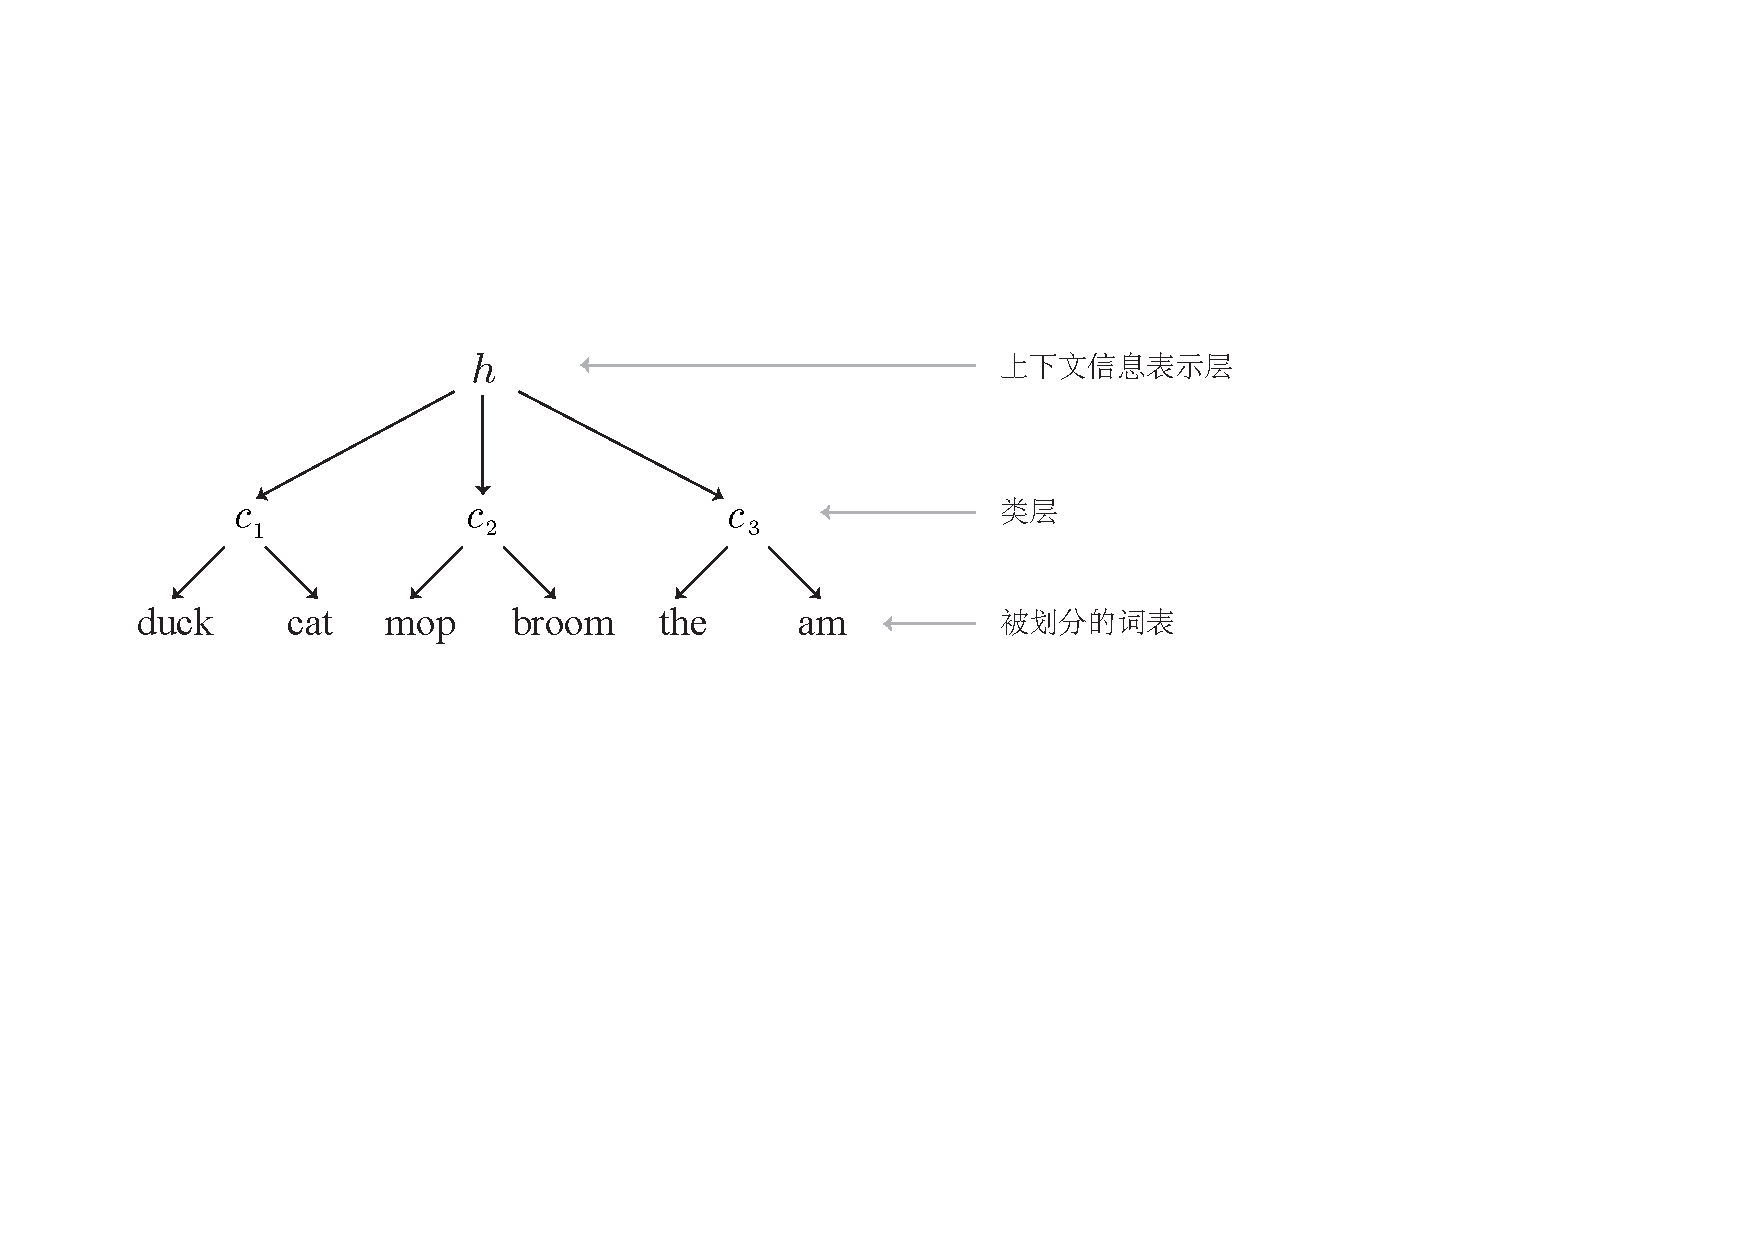
\includegraphics[width=0.79\linewidth]{./figures/case_chsm.pdf}
\caption{cHSM算法可视化模型}\label{fig:case_hsm}
\end{figure}

假设每个类包含 $\sqrt{\mathcal{|V|}}$ 单词,表示词汇被划分为相同大小的组,这样的话级联概率(cascaded probability)只涉及$2\sqrt{\mathcal{|V|}}$ 单词 softmax计算,所以最优时间复杂度可以减少到$\mathcal{O}(\mathcal{|H|}\sqrt{\mathcal{|V|}})$~\upcite{DBLP:conf/icassp/Goodman01}。虽然在更常见的情况下,分区算法会产生不同大小的字组,这需要外部的其他结构来建立高效的数据结构,并且这些稍微复杂的算法尚未被完全探索和分析。此外,我们还可以通过不同的类大小和分区算法来调整精度和效率之间的权衡关系。

另一方面,我们再介绍基于二叉树分解词表的建模策略。tHSM方法将一步多类分类分解为多个二元分类步骤。正因为如此,词汇组织为二叉树,其中单词分布在二叉树的叶子节点上,二叉树的所有的中间节点的都是内部参数。如果该二叉树是平衡树的结构情况下,每个词将会被赋予相等长度的前缀,最优时间复杂度可以减少到$\mathcal{O(|H|\log \mathcal{|V|})}$。最早的工作中,单词在二叉树上的分布可以由WordNet与人类专家~\upcite{DBLP:conf/aistats/MorinB05}或单词 unigram 分布~\upcite{DBLP:conf/nips/MikolovSCCD13}的霍夫曼编码构建。然而,在现实世界的大规模文本应用中,专家知识的构建是相当昂贵的。所以,一般人们也不会采用这样的方案来构建单词的二叉树分布。霍夫曼编码方案只考虑单数据统计,而单词的语境,句法或语义信息尚未被考虑和得到彻底的讨论。

\begin{figure}[!h]
  \centering
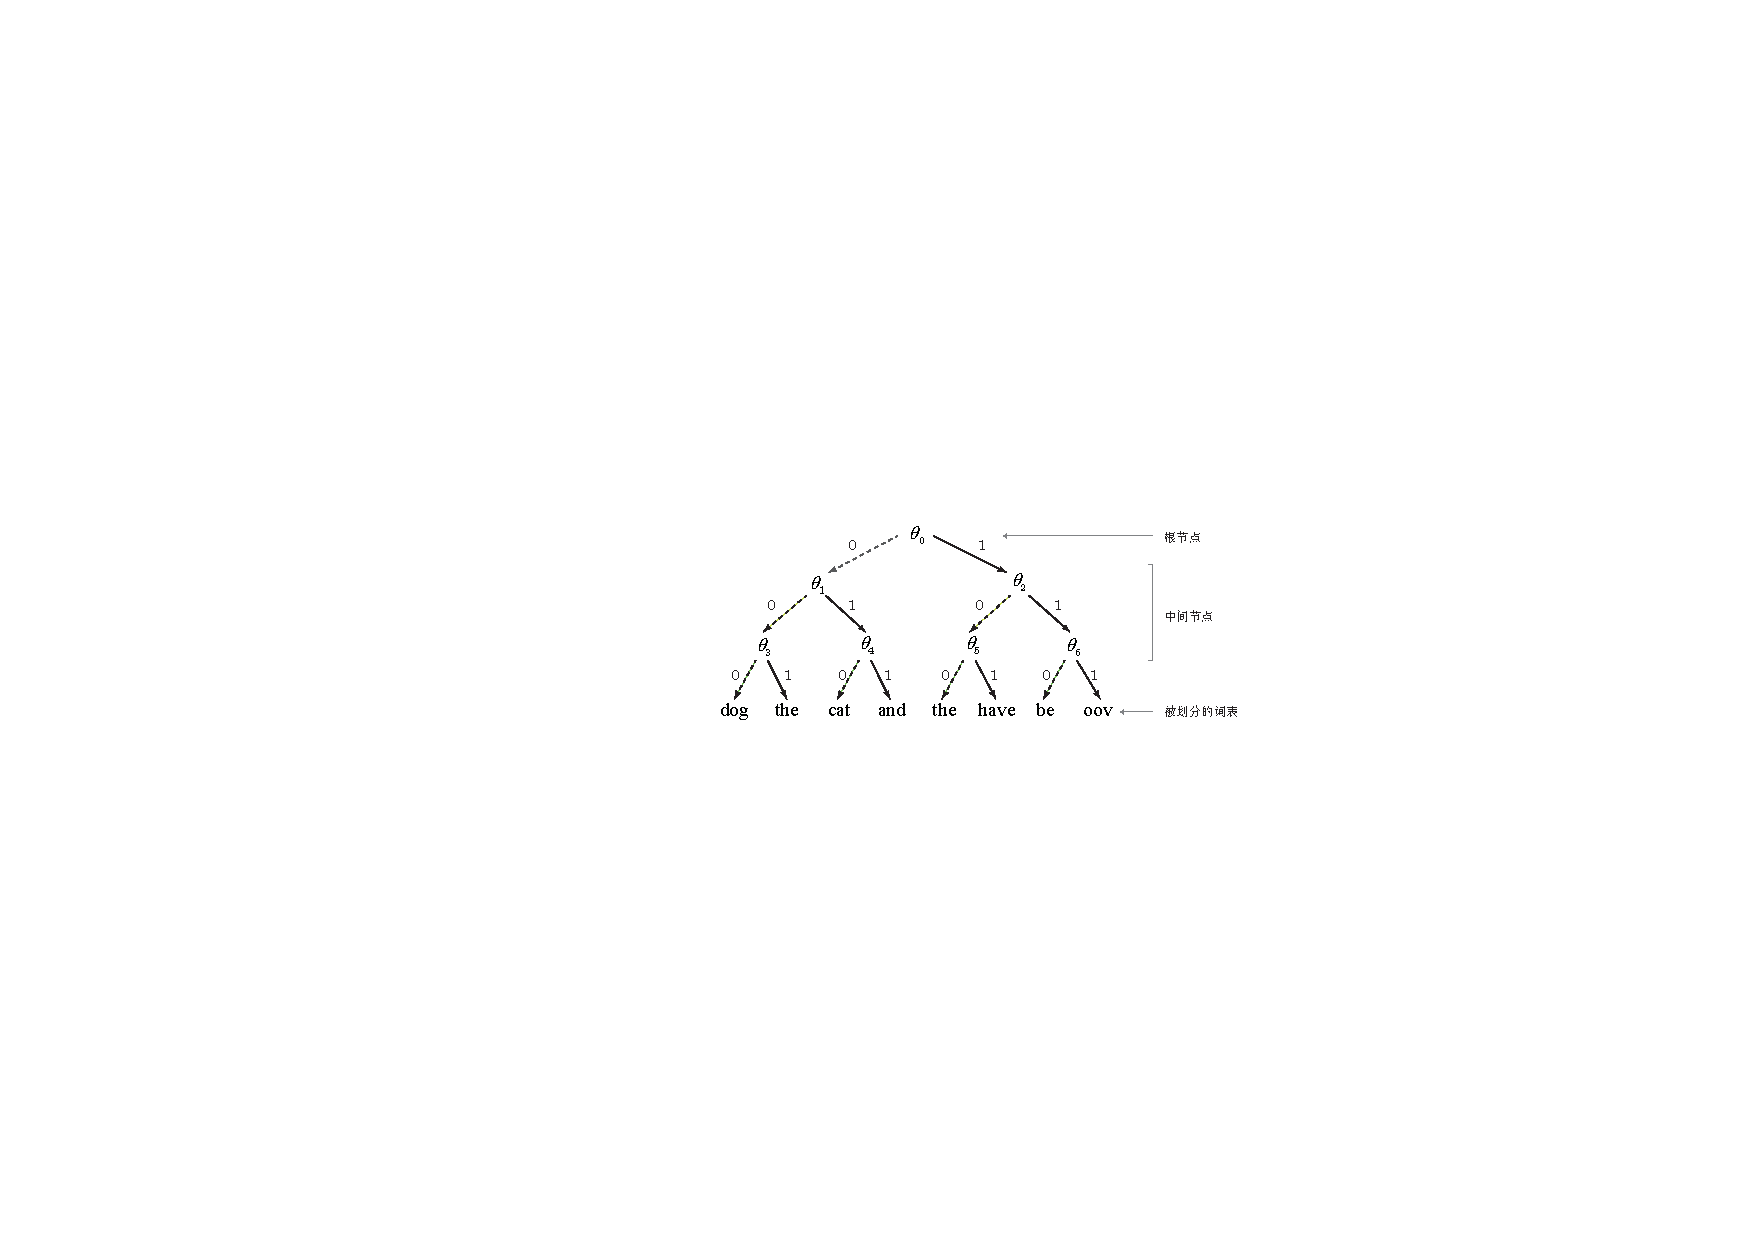
\includegraphics[width=0.9\linewidth]{./figures/thsm-example.pdf}
\caption{tHSM算法可视化模型}\label{fig:case_thsm}
\end{figure}

图~\ref{fig:case_thsm} 展示了二叉树概率分解和计算的示例。

Mikolov当年曾提出使用基于二叉树的层级softmax模型来加速的训练方案,加速比能达到理论的最大速度。但是需要注意的是,当时提出的背景是基于CPU计算方案构建的,如今随着应用领域的推广越来越多的算法应用到实际问题中,我们需要在并行度更高的GPU上进行计算,因此基于GPU进行建模的tHSM和历史上研究众多的cHSM算法尚未被研究提及,因此我们将会需要在本文中详细研讨。

\section{离散采样算法}
在我们使用基于采样的模型时,我们不可避免的需要使用到离散采样函数,即:设一共有$|\mathcal{V}|$个单词,第$i$个单词出现的概率是$p(w_i)$, 如何高效地产生这样的随机变量序列$w_1,w_2,\cdots$?

这问题其实正式来说,可称为模拟离散取样(Simulated Discrete Sampling),跟据有限类别的指定的概率,来模拟取样,生成采样序列输出。其中,要制造指定的概率分布随机变量,关键就是如何通过均匀分布变换获得。因为我们的计算机只能快速产生伪随机数,即均匀分布的采样输出。其他的复杂采样函数均建立在均匀分布的变换之上。
\subsection{随机采样函数}
当我们使用概率模型实现推理和学习算法时,通常需要从离散分布进行抽样。 也就是说,从参数$\boldsymbol {\pi} \in \mathbb{R} ^ K$中的多项式分布,使得$\ pi_k \geq 0$和$\sum_{k} \pi_k = 1$。 更常见的情况是我们在$\mathbb{R}^K$中有一个$\boldsymbol {\phi}$ ,其中$\phi_k \geq 0$,但我们不知道规范化常量。 也就是说,$\boldsymbol{\pi}$只与多项式参数$\boldsymbol {\pi}$成正比。 我们希望根据$\boldsymbol{\pi}$快速生成一个变量,给出$\boldsymbol {\pi}$,用(Matlab)代码很容易地完成某些操作:
\begin{verbatim}
cdf = cumsum(phi);
samp_k = sum(cdf < rand()*cdf(end)) + 1;
\end{verbatim}
这很好很简单,但是你会注意到它具有每个样本的设置(计算CDF)和$\mathcal {O}(K)$时间复杂度的$\mathcal {O}(K)$时间复杂度。每个样本的复杂度可能被降低到$\mathcal {O}(\log K)$,找到阈值的数据结构更好。事实证明,我们可以做得更好,得到$\mathcal {O}(K)$的抽样,而仍然是$\mathcal {O}(K)$。
\subsection{基于线性搜索的逆变换方法}
在上节中,显示了CDF的一些特性,例如CDF的范围是$[0,1]$,而且是一个单调递增的(Monotonic Increasing)函数。逆变换取样算法(Inverse Transform Sampling)就是利用了这些特性,来解决上面提出的问题。其实,逆变换取样方法并不是很复杂,我们接下来详细解释。给一个目标CDF,只要计算其逆函数(Inverse Function),就可以把均匀的随机变数转换为目标CDF:
\begin{equation}\label{equ:func}
  X=F_X^{-1}(Y)
\end{equation}

这方法能用在所有CDF(包括连续及离散的)。其数学证明可参考维基百科。

下图显示这个方法的直观解读,在Y轴范围$[0,1]$里均匀取样$(y_i)$,之后向右和CDF取交点,求交点的$X$轴位置($x_i$),$X$则是符合CDF的概率分布。这个方法用在离散的情况就更简单,只需搜寻目标的CDF,找出超过均匀取样的元素即可。
\begin{figure}[!h]
  \centering
\includegraphics[width=0.5\linewidth]{./figures/cdf.png}
\caption{累计函数采样方法示意图}\label{fig:cdf}
\end{figure}
在离散的情况下(本文题目要求),其时间复杂度是O(N),其中N为类别数目。

读者可能会注意到,这里用了线性搜寻(Linear Search),如果targetPdf数组是由大至小排列,平均而言会更快找到结果。另外,也可以用二分搜寻(Binary Search),那么复杂度会降低为$O(\log |\mathcal{V}|)$,。


\subsection{基于二叉树搜索的逆变换方法}
二分搜索(binary search),也称折半搜索(half-interval search)、对数搜索(logarithmic search),是一种在有序数组中查找某一特定元素的搜索算法。搜索过程从数组的中间元素开始,如果中间元素正好是要查找的元素,则搜索过程结束;如果某一特定元素大于或者小于中间元素,则在数组大于或小于中间元素的那一半中查找,而且跟开始一样从中间元素开始比较。如果在某一步骤数组为空,则代表找不到。这种搜索算法每一次比较都使搜索范围缩小一半。

事实上,这个问题用二分搜寻是标准的方法。那么,还有没有更快的方法呢?答案是肯定的,例如别名方法(alias method)、近似方法等~\upcite{DBLP:journals/cgf/ClineRW09}。当然,在N很小的情况下,线性搜寻和二分搜寻也足够。
\subsection{别名方法}

设$ Z $为离散的随机变量,它有n个可能的结果$ z_0,z_1,\ldots,z_ {n-1} $。 为了简化下面的讨论,我们研究另一个变量$ Y $,其中$ P \{Y = i \} = P \{Z = z_i \} $。 当$ Y $取值$ i $时,让$ Z $为$ z_i $。 所以$ Z $可以从$ Y $生成。随机变量$ X $被均匀分布在$(0,n)$中,这个概率密度函数是
\begin{equation}\label{equ:alias}
 f(x) = \left\{
 \begin{array}{rl}
  1/n & \text{若 } 0 < x < n\\
  0 & \text{否则}\\
 \end{array} \right.
\end{equation}
那么我们现在生成的$Y'$是:
\begin{equation}\label{equ:gen}
  Y' =  \left\{
 \begin{array}{rl}
  \lfloor x  \rfloor & \text{若 } (x - \lfloor x \rfloor) < F(\lfloor x \rfloor)\\
  A(\lfloor x \rfloor)  & \text{否则}\\
 \end{array} \right.
\end{equation}
其中$ A(i)$是别名函数。 当$ x $落入范围$ [i,i + 1)$($ i $是一个整数)时,$ y $的概率$ F(i)$为$ i $,概率$ 1 - F(i )$是$ A(i)$。 由于$ x $是均匀分布的,
\begin{equation}
  \begin{split}
P\{x \in [i, i + F(i))\}     &= \int_i^{i+F(i)}\frac{1}{n}dx= (i + F(i) - i) \times 1/n= F(i)/n,\\
P\{x \in [i + F(i), i + 1)\} &= \int_{i+F(i)}^{i+1}\frac{1}{n}dx= (i + 1 - (i + F(i))) \times 1/n= (1-F(i))/n
\end{split}
\end{equation}

让我们将满足$ A(j)= i $的值集合$ j $表示为$ A ^ { - 1}(i)$。 生成的变量$ Y'$具有以下概率质量函数:
\begin{equation}
  P\{Y' = i\} = F(i)/n + \sum_{j \in A^{-1}(i)}\frac{1-F(j)}{n}
\end{equation}
Alias方法是构造$ A $和$ F $的算法,所以$ P \{Y'= i \} $等于$ P\{Y = i \} $。 由于$ A $和$ F $的域都是整数$ 0,1,\ldots, n-1 $,所以它们可以存储在数组中,并且可以在$O(1)$中查找值,其中空间效率是 $\mathcal{O}(n)$。

虽然别名方法可用于生成丰富的噪声字,因为它需要线性建立时间和恒定的采样时间~\upcite{10.2307/2683739,DBLP:conf/emnlp/VaswaniZFC13}。

大词表问题,主要是对softmax如何建模的问题。在本课题中,我们探讨 cHSM 和 tHSM 两种不同的方案所带来的影响和优劣。
\section{本章小结}
本章对国内外学者在语言模型的任务上相关工作进行了介绍。首先,介绍了语言模型的建模策略和对应的应用方案。并详细讨论了循环神经网络的语言模型的建模方式,并讨论了其结构的优缺点。同时为了解决使用循环网络所带来的梯度爆炸的问题,我们进而引入了长距离短期神经网络和门限记忆节点两种基于门限机制的循环网络;另一方面,我们还考虑了语言模型大规模应用所带来的大词表问题,并作了详细分析其原因。为了解决该问题,我们还讨论了历史上所提出的方案,并做了分类讨论。主要涉及三种思路:缩减词表大小,用采样算法近似估计和模型层次分解。针对各种模型提出的结果做了详细介绍,并分析了各种算法的优劣处。最后我们分析了实验中需要用到的高效采样函数的构造算法。
\RestyleAlgo{boxed}
\chapter{并行树状概率计算模型}
\section{引言}
在本章中,我们将这个预测端的词用二叉树的分层的形式表示,使它们的编码适配基于树的分层概率计算。首先,我们提出了一个在分层结构上建模参数的字编码方案。因为考虑到GPU上的算法的并行计算的吞吐性能,我们进而推导出紧凑的代价函数及其梯度,使得模型在GPU设备上的能并行计算模型的内部概率函数。

同时,树上的单词分布对其性能有很大的影响,应该在训练阶段之前定义。在本实验中,我们并不打算考虑那些在训练过程中动态交换子树的算法进而改变了单词在子树上的分布结构, 而是我们采用了几个分层聚类策略,用统计,句法和语义知识来初始化其结构,以达到一个稳定和可以预期的性能。

另外,在模型的测试推理过程中,不同于传统的softmax算法情况,得到最好的候选者自然是可行的并且能直接被计算出来,层次推理模型不能直接应用 softmax 方法来实现。因此我们讨论了基于二叉树的搜索策略,以满足两种不同的推理情情形:a)给句子打分。输出给定序列的概率;b)给定上下文,对文本进行排序。在给定的上下文中获取得分最高的一个候选单词。
\section{基于二叉树的单词极性编码}
首先,所有的单词分布在二叉树的叶节点上,因此我们可以通过访问从根到叶节点的所有内部节点来定位每个特定的词,所以不同的访问路径代表不同的单词。在这里,单词$ w $的路径表示所有内部节点$ \theta^w_i $和它访问的边$ d ^ w_i $。

\begin{table}[!ht]
  \centering
  \caption{并行树状概率计算模型的符号助记表}
\begin{tabular}{llc}
  \toprule
   符号&涵义&取值范围\\ \midrule
$l^w$ &单词$w$ 所对应的叶子节点和中间节点的路径&Int32 \\
$d_j\in \{-1,+1\}$&表示路径$l^w$中第$j$个节点对应的编码(根节点对应编码$0$)&\\
$ d^w=[d_0^w,d_1^w,\cdots,d_{l^w-1}^w] $& 单词 $w$ 的极性编码,他由 $l^w-1$位编码构成,&\\
$\theta_{j}^w\in\mathbb{R}^m$ &表示路径$l^w$中第 $j$ 个非叶子节点对应的向量& Float32\\
$ \theta^w=[\theta_1^w,\theta_2^w,\theta_3^w, \cdots,\theta_{l^w}^w]$&表示路径$l^w$所对应的参数矩阵&Float32 \\
$\Gamma$ &路径查找表,给定路径序列,可以获得对应的单词& \\
  \bottomrule
\end{tabular}
\end{table}

我们接下来详细说明模型的编码方式。其中,$ \theta_i ^ w $表示到达单词$w$的路径上的$ i^{th} $层上的非叶节点,并且$\theta_i ^ w$是一个 $m$维度的向量,$ \theta_i ^ w \in\mathbb{R}^m $ 其中$ i \in [0, l ^ w - 1] $。同样的,$ d_i ^ w $表示连接第$(i-1)^ {th} $和$ i ^ {th} $层节点的边。对于每个非叶子节点来说,向下移动到左边的分支标记为$ -1 $,选择正确的分支标记为$ + 1 $。因此,在$i\in[0,l^w-1]$, $d_i^w\in \{-1,+1\}$。 此外, $l^w$~表示从根到叶单词的路径长度。如果该二叉树是平衡树,即单词都均匀分布在同一层叶子节点上,那么树深是$l^w\approx \log \mathcal{|V|}$ 。通过这个方案,我们可以通过表示极性路径来定位每个单词,将单词索引(Indexing)或二元稀疏表示(One-hot Representation)改变为单词极性编码元组$(d ^ w,\theta ^ w)$。


在用python语言实现过程中,我们通过维护一个路径查找表$\Gamma$(Lookup Table),记住每个单词$ w $从根到叶的所有访问内部节点的索引。这样,通过从$ \Gamma(w)$中选择对应行的所有节点,从参数矩阵${\Theta} $中检索$ \theta ^ w $。其中${\Theta} $的第一维的维度是:
\begin{equation}\label{equ:sums}
\sum_{i=0}^{\log \mathcal{|V|}}{2^i} = \mathcal{|V|} -1.
\end{equation}
因此,p-tHSM模型没有增加模型额外参数,除了预先给定的路径查找表$ \Gamma $。

除此以外,我们通过从矩阵$\mathcal{D}$中获得$w^{th} $行向量来检索$d^w$,其中$w$是词汇表中的单词索引。 此外,$\{\Gamma,\mathcal{D}\}$ 是由层次聚类算法预先给定的,$\Theta$是通过训练数据集上的代价函数的梯度下降来优化的。为了保证理解正确,我们在这里再一次强调$ \Theta $是模型的参数,$ \Gamma $记忆路径节点索引信息,$\mathcal {D}$取 $ \{ - 1,+1 \} $中的值。

如图~\ref{fig:tree_hsm}~所示,内部参数向量 $\theta_i^w$, 边 $d_i^w$ 并且单词在树的叶子节点上。除此之外, 加粗的那条路径从根节点到叶子节点 $w$ 被定义为参数对 $(d^w,\theta^w)$。其中 $d^w$ 是一个向量, $\theta^w$ 是一个参数矩阵. 例如, 图里面的参数实际结果是 $d^w=[-1,+1,-1]$ , $d^{v}=[-1,+1,+1]$。
\begin{figure}[!h]
  \centering
    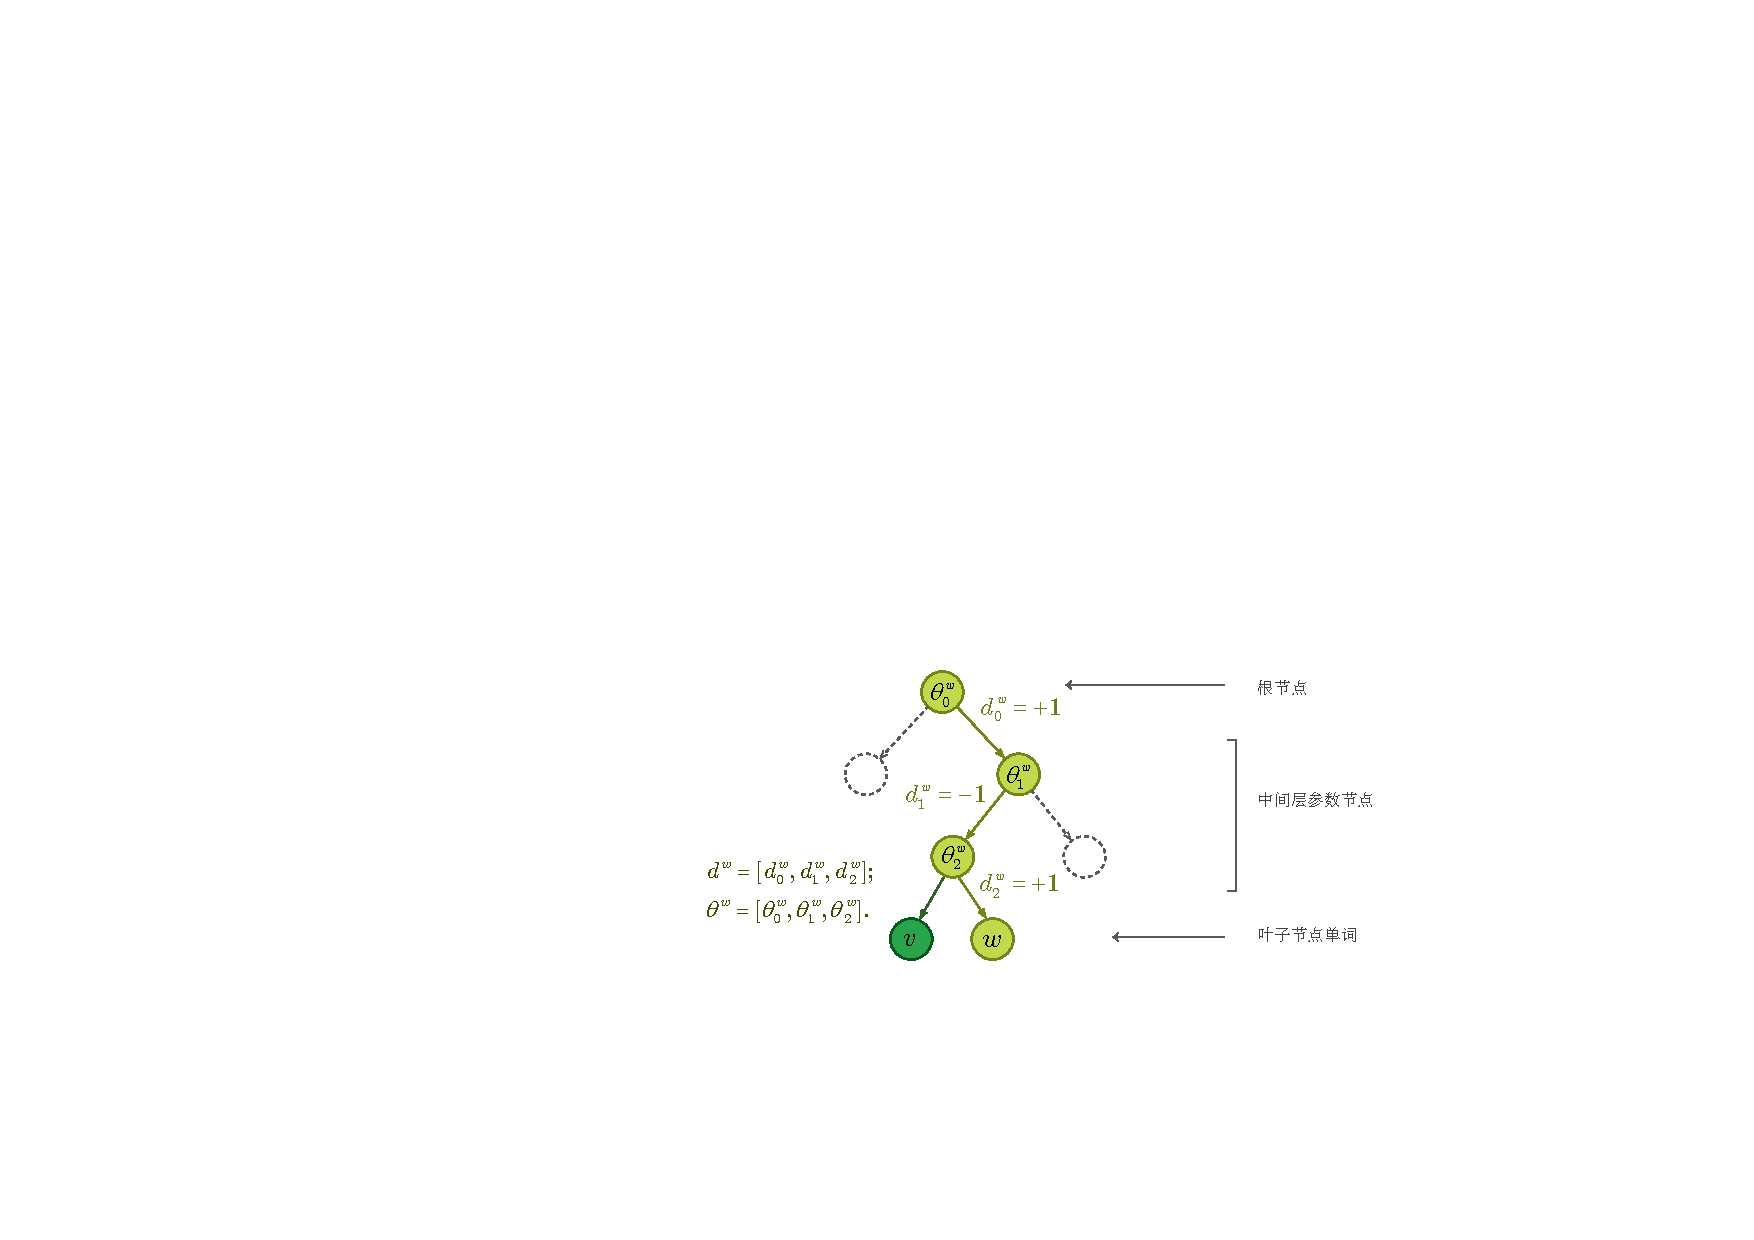
\includegraphics[width=0.8\linewidth]{./figures/thsm.pdf}
\caption{树状层次概率模型}\label{fig:tree_hsm} %
\end{figure}

\section{基于二叉树的代价函数和导数}
在目标词树的每个步骤中,我们对每个非叶节点是左下分支还是右分支进行逻辑预测。 所以当我们给定$ i^{th} $节点和隐藏层$ h $的$ i^{th} $的时候,我们可以计算标签 $d^w_i\in \{-1,1\}$的概率为:
 \begin{equation}\label{equ:pp}
p(d^w_i|\theta_{i}^w,h) =\sigma(\theta_{i}^w h)^{d_i^w}\times(1-\sigma(\theta_{i}^w h))^{1-{d_i^w}},d_i^w \in [0,1]
\end{equation}
其中$ \sigma(z)= 1 /(1 + \exp(-z))$表示 $\sigma$ 函数。根据 $\sigma$ 函数的对称性规则:$\sigma(z)+ \sigma(-z)=1 $,以下是该公式的证明过程:
\begin{equation}\label{equ:sig}
\begin{split}
\sigma(z)+ \sigma(-z)  &=\frac{1}{1 + \exp(-z)}+\frac{1}{1 + \exp(z)}\\
  &=\frac{\exp(z)}{1 + \exp(z)}+\frac{1}{1 + \exp(z)}=\frac{1 + \exp(z)}{1 + \exp(z)}=1
\end{split}
\end{equation}
该规则可以用来帮我们把公式~\ref{equ:pp}~缩写成一下更简洁的形式~\upcite{minka2003algorithms}:
 \begin{equation}
p(d^w_i|\theta_{i}^w,h) =\sigma(\theta_{i}^w h)^{d_i^w}, d_i^w \in [-1,+1]
\end{equation}
由于公式中的其中某一项${d_i^w}$是在指数项上面,所以我们尽管做了这个基于$\sigma$函数的变换,我们的计算公式仍然不是最佳的形式,还是有空间来提升共识的紧凑性保证计算时的高并行度。更进一步的讲,我们可以将上面的公式缩写成以下形式:
\begin{equation}
p(d^w_i=\pm 1|\theta_{i}^w,h) = \sigma({d_i^w}\theta_{i}^w h)
\end{equation}
这样的操作之后,我们就完成了单节点概率计算的紧凑表示。针对计算一个单词的概率,我们需要考虑从根节点到该单词叶子节点的所涉及的所有层的概率公式。然而因为在训练的时候,我们实际上预先知道每个单词所对应的路径,所以我们实际上可以同时的计算各个节点的概率值,然后将所有节点相乘起来。这样做的好处,现在看起来十分费力,但是我们可以在下面详细说明。

 因此,我们传统意义上计算的单词的概率在这里指的是:单词$ w $在二叉树上的概率,即从根到相应叶节点的路由概率$(d^w,\theta^w)$的联合乘积:
\begin{equation}\label{equ:pw}
\begin{split}
 \log p(w|h)=&\log\prod_{i=0}^{l^w-1} p(d^w_i|\theta_{i}^w,h) = \sum_{i=0}^{l^w -1} \log\sigma(d_i^w \theta_{i}^w h)\\
 =&\log\sigma({d^w}^\top \theta^w h)=\zeta(- {d^w}^\top \theta^w h )
 \end{split}
\end{equation}
其中 $\zeta(z)$ 代表 softplus 函数: $\zeta(z)= \log (1+\exp(z))$。 该函数的导数是 $\sigma$ 函数, 其导数计算公式是: ${\mathrm{d}\zeta(z)}/{\mathrm{d} z}= \sigma(z)$~\upcite{DBLP:conf/nips/DugasBBNG00}。如图所示, softplus 函数通常被视为 ReLU函数的替代函数,因为他们两个函数除了零点附近分布不一样以外,其他地方分布相同。但是softplus函数在零点附近可导,ReLU函数在零点附近不可导。
\begin{figure}[!ht]
  \centering
\includegraphics[width=0.6\linewidth]{./figures/relus.pdf}
\caption{Softplus和ReLU函数的示意图}\label{fig:soft}
\end{figure}

接下来,我们给出模型相应的损失函数$ \ell(\theta | h,w)$,它是定义在二叉树上面的负对数似然函数(Negative Log-Likelihood,NLL):
\begin{equation}\label{equ:cost}
\begin{split}
   \ell(\theta|h,w) =&-\log\prod_{i=0}^{l^w -1} \sigma(d_i^w \theta_{i}^w h) = -\log \sigma({d^w}^\top \theta^w h)\\
    =& \log (1+\exp(- {d^w}^\top \theta^w h )) =  \zeta(- {d^w}^\top \theta^w h )
\end{split}
\end{equation}
从此公式中,我们可以发现最小化基于树的负对数似然值,意味着直接最大化softplus损失和估计字的概率。

尽管如此,在传统的tHSM算法中,该模型逐层计算每个节点的对数概率。 因此,这个词的整体联合对数概率通过各层线性相加。 因此tHSM的时间复杂度为$\mathcal{O(|H|\log|V|})$,其计算公式为:
\begin{equation}
\ell(\theta|h,w) =\sum_{i=0}^{l^w-1} \{(1-d'^w_i)\log (\sigma(\theta_{i}^w h))  + {d'^w_i}\log (1-\sigma (\theta_{i}^w h))\}
\end{equation}
其中 $d'^w_i\in \{0,1\}$,这两个部分从底到顶,分别对内部节点的左右子树的联合概率进行建模。

值得注意的是,p-tHSM和tHSM算法之间的主要区别在于:a)tHSM算法涉及许多微小的矩阵乘法操作,而在p-tHSM中我们直接将所有参数$(d^w,\theta^w)$ 2D矩阵是以运行时内存消耗为代价的,我们考虑这个向量和相对较大的矩阵的乘法,如图~\ref{fig:tree_hsm}~所示。 b)扣除模型的紧凑损失函数,并行的计算这条路径上所有节点的对数概率而不是逐层计算,为p-tHSM模型提供更好的时间效率。

接下来,模型的所有参数$\{\theta^w,h\}$针对模型的代价函数的导数是 :
\begin{equation}
\begin{split}
\frac{\partial \ell}{\partial \theta^w}=&(\sigma({d^w}^\top\theta^w h) -1){d^w}^\top h \\
\frac{\partial \ell}{\partial h}=&(\sigma({d^w}^\top \theta^w h) -1){d^w}^\top \theta
\end{split}
\end{equation}


二叉树分解的一个主要优点是它避免了在整个词汇表中概率的归一化,因为树中词的汇总概率自然等于1。
\begin{equation}
\sum_{w\in \mathcal{V}}{p(w|h)}=\sum_{w \in \mathcal{V}}\sum_{i=0}^{l^w-1}{\sigma(d_i^w\theta_{i}^w h)}=1.
\end{equation}



\section{基于二叉树的推理算法}
考虑到本章开始提出的第一个问题,即给定序列$ [w_1,\cdots,w_T] $,求该序列出现的概率。 直观地说,当给定相应的上下文$ h $时,我们可以通过获取一个特定单词$ w $的概率或对数概率来分解问题:
\begin{equation}
\begin{split}
    p(w|h) =&\sigma({d^w}^\top \theta^w h)\\
   \log p(w|h) =& -\zeta(- {d^{w}}^\top \theta^{w} h )
\end{split}
\end{equation}
其中概率$ p(w | h)$和单词$ w $的对数概率$ \log p(w | h)$可以直接通过等式~\ref{equ:pw}~和~\ref{equ:cost}~逐步计算出来。 因此,我们可以推导出这个序列的概率为:
\begin{equation}
   \log p(w_1,\cdots, w_T)=\sum_{t=1}^T\log p(w_t|h_t) = -\zeta(- {d^{w_t}}^\top \theta^{w_t} h_t )
\end{equation}
显然,这种类型的操作比传统的softmax方法有效得多,因为它只需要$\mathcal{O}(\mathcal {| H | \log| V |})$计算复杂度,而传统的softmax算法却需要$\mathcal{O}(\mathcal {| H || V |})$。

关于第二种情况(也被称为$\arg\max $方法),即当给定前一个上下文时,在整个词汇表中搜索最有可能的下一个单词(概率最大的单词)。我们可以在选择最上面的一个候选人之前计算词汇表中所有单词的概率。这个过程仍然是昂贵而缓慢的,因为它涉及到整个词的分层树。如在算法~\ref{alog:argmax}~中所描述的,为了避免两个小概率的精确度损失问题,我们选择计算每个内部节点的对数概率。

而不是搜索全局最优结果,我们可以用局部贪婪算法搜索次优结果。具体而言,对于$ i $ -th层中的节点,当$ p(d ^ w_i | \theta_{i} ^ w,h)\ge 0.5 $时选择左边的分支,相反适用,如算法~\ref{alog:greed_argmax}所示。因此,计算时间复杂度仍然是$ \mathcal{O}(| H | \log \mathcal {| V |})$。


\begin{algorithm}[!ht]
\SetAlgoLined
\KwData{隐藏层输出 $h$;}
 路径列表 $\mathtt{route}$=[] \;
\While(\tcp*[h]{逐层贪心路径搜索}){$k \le \log \mathcal{V}$ }{
\eIf{$p(d_{k} |\theta_{k},h) \ge 0.5$ }{
 $k=  k*2$ \tcp*[r]{左分支}
}{
 $k = k*2+1$ \tcp*[r]{右分支}
}
 $\mathtt{route}$.add($k$) \tcp*[r]{将 $k$ 添加到路径列表}
}
{通过查找$\Gamma$路径表,找出对应的单词}\;
$w=\Gamma(\mathtt{route})$\;
\KwResult{ 预测的单词 $w$. }
\caption{逐层贪心搜索算法}\label{alog:greed_argmax}
\end{algorithm}


\begin{algorithm}[!ht]
\SetAlgoLined
\KwData{隐藏层输出 $h$;}
 路径列表 $\mathtt{path}$=[] \;
\While(\tcp*[h]{全局概率计算函数}){$k \le \log \mathcal{V}$ }{
\eIf{$p(d_{k} |\theta_{k},h) \ge 0.5$ }{
 $k=  k*2$ \tcp*[r]{左分支}
}{
 $k = k*2+1$ \tcp*[r]{右分支}
}
 $\mathtt{path}$.append($k$) \tcp*[r]{将 $k$ 添加到路径列表}
}
{通过查找$\Gamma$路径表,找出对应的单词}\;
$w=\Gamma(\mathtt{path})$\;
\KwResult{ 预测的单词 $w$. }
\caption{全局单词最优算法}\label{alog:global}
\end{algorithm}

\section{基于二叉树的聚类算法}
词汇表中每个单词$(d^w,\theta^w)$的极性编码与树的结构密切相关。因此对于提出的p-tHSM算法,我们采用了多种树聚类算法来初始化单词在二叉树上的分布,以提高左后模型的精确性和稳定性。总的来说,这些聚类算法为每个单词生成二进制前缀字符串,表示树中单词的位置,并将用于初始化p-tHSM方法。


1)一元聚类算法。它根据词频对词汇进行排序,并根据单词统计从底端到顶端进行合并,也称为霍夫曼编码~\upcite{DBLP:conf/nips/MikolovSCCD13}。

霍夫曼编码的构造过程。1) 根据$\mathcal{|V|}$个权值$\{w_1,w_2,\cdots,w_{\mathcal{|V|}}\}$,生成$\mathcal{|V|}$棵只有单个结点的树,没有左右子树的二叉树的集合$F\{T_1,T_2,\cdots,T_{\mathcal{|V|}}\}$,其中每颗树的根节点都有一个权值$w_i$;2) 在~$F$~中选取两颗根节点的权值最小的树作为左右子树构造一颗新的二叉树。对于这两颗子树,权值小的作为左子树,权值大的作为右子树。新的二叉树的权值是两颗子树的权值之和;3)将2步选取的两颗树在$F$中删除,并将新二叉树加入$F$中。4)重复2,3步,直到~$F$~中只有一颗树为止。

\begin{algorithm}[!ht]
\SetAlgoLined
\KwData{单词和对应的频度词典 frequenties;}
{Q=PriorityQueue()} \tcp*[r]{初始化优先队列$Q$}
\For(\tcp*[h]{((freq,word),index)}){$v \gets frequenties$}{
{Q.put(v)}\;
}
{$idx=0$}\;
\While{$Q.qsize()>1$}{
    {l,r=Q.get(),Q.get()}\;
    {node=Node(l,r,idx++)}\;
    {freq=l[0]+r[0]}\;
    {Q.put((freq,node))}\;
}
\KwResult{ 霍夫曼树 $Q.get()[1]$. }
\caption{基于单词频率的霍夫曼建树策略}\label{code:huffman}
\end{algorithm}

当我们构造完霍夫曼二叉树后,我们需要遍历这棵树来获取所有单词的极性编码霍夫曼编码:1)计算待压缩数据中所有的字符及其出现次数,根据次数的不同对没个字符分配不同的权值(一般用出现频率/总字符数)。2)对所有带压缩字符按起权值,构造一颗霍夫曼树。3)对这棵树所有子树的左支用$-1$编码,右支用$+1$编码。每个位于叶子节点的字符的编码为从根节点到该叶子节点路径上的$-1,+1$编码值,这个在这棵树上重新得到的编码叫霍夫曼编码。这样可以得到每个字符的极性编码。
\begin{algorithm}[!ht]
\SetAlgoLined
\KwData{单词和对应的频度词典 frequenties;}
collector=[], polarity=[], param=[]\;
\If{self.left}{
    \eIf{isinstance(self.left[1],Node)}{
          {self.left[1].preorder(polarity+[-1],param+[self.index],collector)}\;
    }{
          {collector.append((self.left[1],param+[self.index], polarity + [-1]))}\;
    }
    }
    \If{self.right}{
        \eIf(\tcp*[h]{右子树存在}){isinstance(self.right[1],Node)}{
          self.right[1].preorder(polarity+[1],param+[self.index],collector)
        }{\tcp*[h]{左子树存在}\;
          collector.append((self.right[1],param+[self.index], polarity + [1]))
          }
    }
\KwResult{ 单词路径查找表 $\gamma$. }
\caption{前序遍历函数生成单词路径查找表}\label{code:preorder}
\end{algorithm}
如图~\ref{fig:zipf}~所示,我们算法中用到输入信息$frequenties$指的是单词的词频分布。
\begin{figure}[!ht]
  \centering
\includegraphics[width=0.6\linewidth]{./figures/zipf.png}
\caption{单词 Unigram分布示意图}\label{fig:zipf}
\end{figure}

其对应的二叉树的数据结构采用基于数组的方式管理和访问。如下所示,每个节点(Node)包含信息为:左子树,右子树,节点编号。同时我们还定义了节点的打印字符串函数(即``repr''),方便我们检查数据结构是否正确实现。
\begin{minted}[mathescape,linenos=False,gobble=1,frame=lines,baselinestretch=1.0,fontsize=\footnotesize,framesep=1mm]{python}
 class Node(object):
  def __init__(self,left=None,right=None,index=None):
   self.left=left
   self.right=right
   self.index=index

  def __repr__(self):
   string=str(self.index)
   if self.left:
    string+=', -1:'+str(self.left.index)
   if self.right:
    string+=', +1:'+str(self.right.index)
   return string
\end{minted}


2)二元聚类算法\footnote{布朗聚类:https://github.com/percyliang/brown-cluster}。它是一个层次聚类算法,使用bigram上下文来确定单词的分布相似性,将相似的单词放置在二叉树的附近位置~\upcite{DBLP:journals/coling/BrownPdLM92,liang2005semi}。在将簇大小指定为1之后,它从底部到顶部合并具有一个节点的单词。生成的单词二进制路由正是分层二进制结构的分布。
\begin{figure}[!ht]
  \centering
\includegraphics[width=0.6\linewidth]{./figures/brown.png}
\caption{布朗聚类分布示意图}\label{fig:brown}
\end{figure}

3)语义信息聚类算法\footnote{https://code.google.com/archive/p/word2vec/}。在引导式的方式下,词嵌入在外部语料库上训练,我们将传统的凝聚式聚类应用于字嵌入特征~\upcite{DBLP:books/sp/mining12}。


\section{本章小结}
本章首先定义了极性编码的概念,同时给出了模型所涉及的参数的详细涵义。接下来,我们逐步推导模型的单个节点的概率公式,单个词的概率公式和模型的代价函数。另一方面,我们将提出的p-tHSM算法和传统的线性tHSM算法进行的比较。通过比较两者计算的差异性证明我们提出的算法更适合在GPU等高并行设备上运算。进一步的,我们还讨论了模型在测试的时候所需的推理算法,因为基于二叉树的概率计算方案和传统的softmax计算方案不同,不能直接输出单个词的概率或者计算最佳的候选单词,所以我们分别针对这两个任务提出推理算法。最后,由于单词在二叉树上的分布需要初始化,我们讨论了传统的霍夫曼聚类算法,布朗聚类算法和语义向量聚类算法,并给出了三种算法的详细计算过程。

\RestyleAlgo{boxed}
\chapter{类别层次概率计算模型}
上一章介绍了将预测端的词用二叉树的分层的形式表示,本章将这个目标词表示扩展到类别的形式,并讨论基于类别划分的层次概率模型。首先本章提出在划分的类别结构上建模的单词编码方案,进而推导出该模型的代价函数及其梯度。同时在实验中注意到类别划分的单词分布对模型的性能有很大的影响,应需要在训练阶段之前被定义,所以本文考虑几种现有的词表分割策略,包括:基于单词或者文本的统计、句法和语义知识来划分其层次结构,使模型能达到稳定和高效的结果。在模型推理过程中,本章针对两种不同的情况:1)打分:输出给定序列的概率;2)排序:在给定的上下文中获取得分最高的候选单词,分析并提出可能的优化策略。


\section{词表划分编码}
\begin{table}[!ht]
  \centering
  \caption{类别层次概率计算模型的符号助记表}
\begin{tabular}{llc}
  \toprule
   符号&含义&取值范围\\ \midrule
$\theta^c\in\mathbb{R}^m$ &表示单词的类别向量& Float32\\
$ \theta^o$ &表示路径$l^w$表示划分后的单词三维张量&Float32 \\
$\Gamma'$ &路径查找表,给定单词元组序列,可以获得对应的单词&--- \\
  \bottomrule
\end{tabular}
\end{table}
词表分割算法能将词表划分成多个大小不均匀的分组,传统的类别层次模型仅能计算均匀划分后的单词概率,为了支持广义的词表划分算法,本章提出基于词表划分的元组编码方式。

首先介绍非均匀划分的词表的编码方式,词表被表示成:类别向量~$\theta^c$~和划分的单词矩阵~$\theta^o$。其中前者定义了类别层的概率~$p^c$~,而后者表示该分组内的单词局部概率~$p^o$,如图~\ref{fig:unequal}~所示。其中,划分的单词矩阵的维度是:类维度和分组词维度。如果将词表~$\mathcal{V}$~划分为不等大小的组,则需要将单词矩阵分类为等长矩阵,对于不在这个组中的剩余节点,我们使用零掩码~$\theta^m$来消除其对局部单词概率和总代价函数的影响。
因此,分组词维度是最大的组长度。如果应用词表均匀分割的算法(如图~\ref{fig:equal}~所示),掩码向量~$\theta^m$~可以被忽略,并且分组词维度是~$\mathcal{|V|/|C|}$(~$\mathcal{|C|}$~表示类维度)。另外,如果~$\mathcal{|V|}$~不能被~$\mathcal{|C|}$~整除,那么最后的分组包含实际的单词数量应该小于该组的大小。考虑到这样的不存在的单词占据很少一部分,同时不影响其他类别的概率计算,实际的影响比较小,所以掩码向量~$\theta^m$~可以被忽略。
\begin{equation}\label{equ:partition}
 \theta^m=
\begin{cases}
    \text{单位矩阵,}& \text{若均匀划分} \\
    \text{掩码矩阵,} & \text{否则}
\end{cases}
\end{equation}

\begin{figure}[!ht]
  \centering
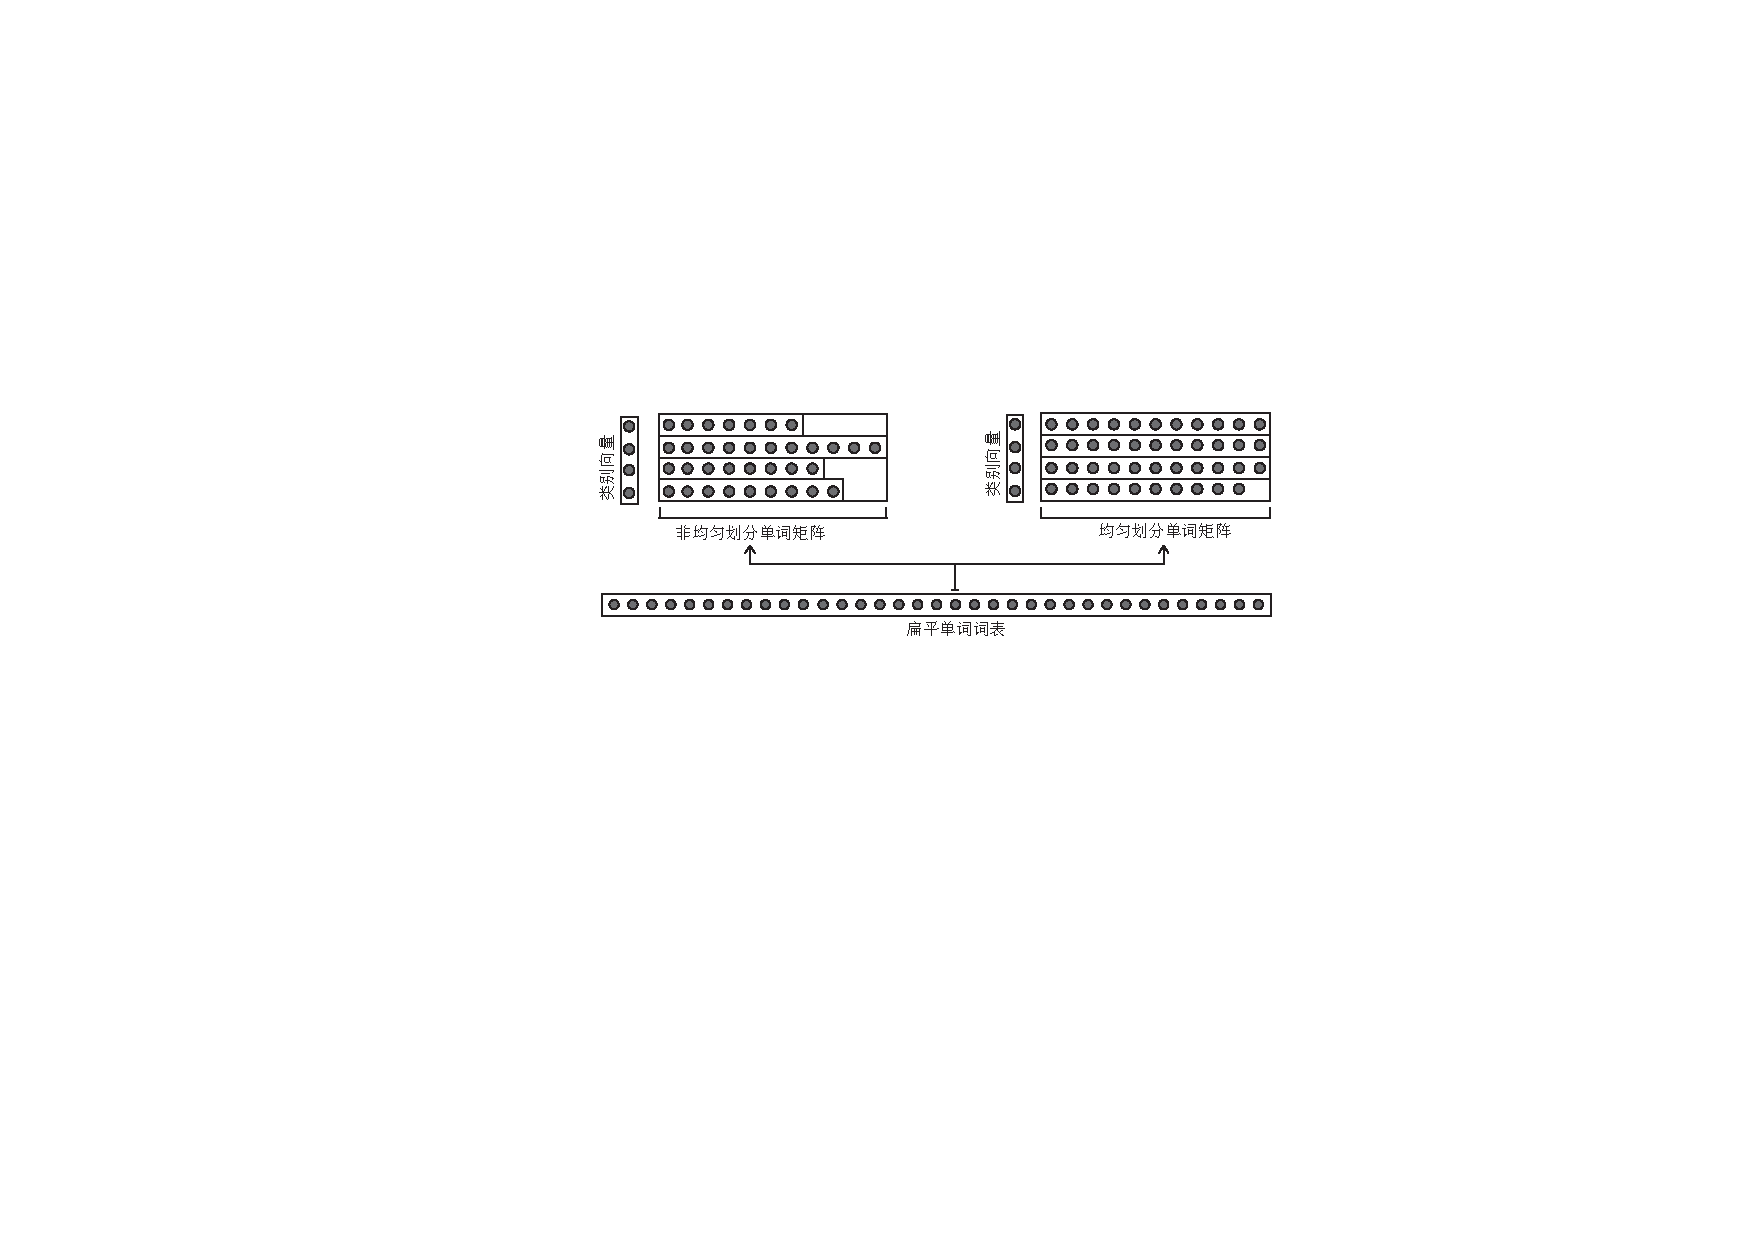
\includegraphics[width=.9\linewidth]{./figures/chsm-simple.pdf}
\caption{非均匀词表划分结构示意图}\label{fig:unequal}
\end{figure}
\begin{figure}[!ht]
  \centering
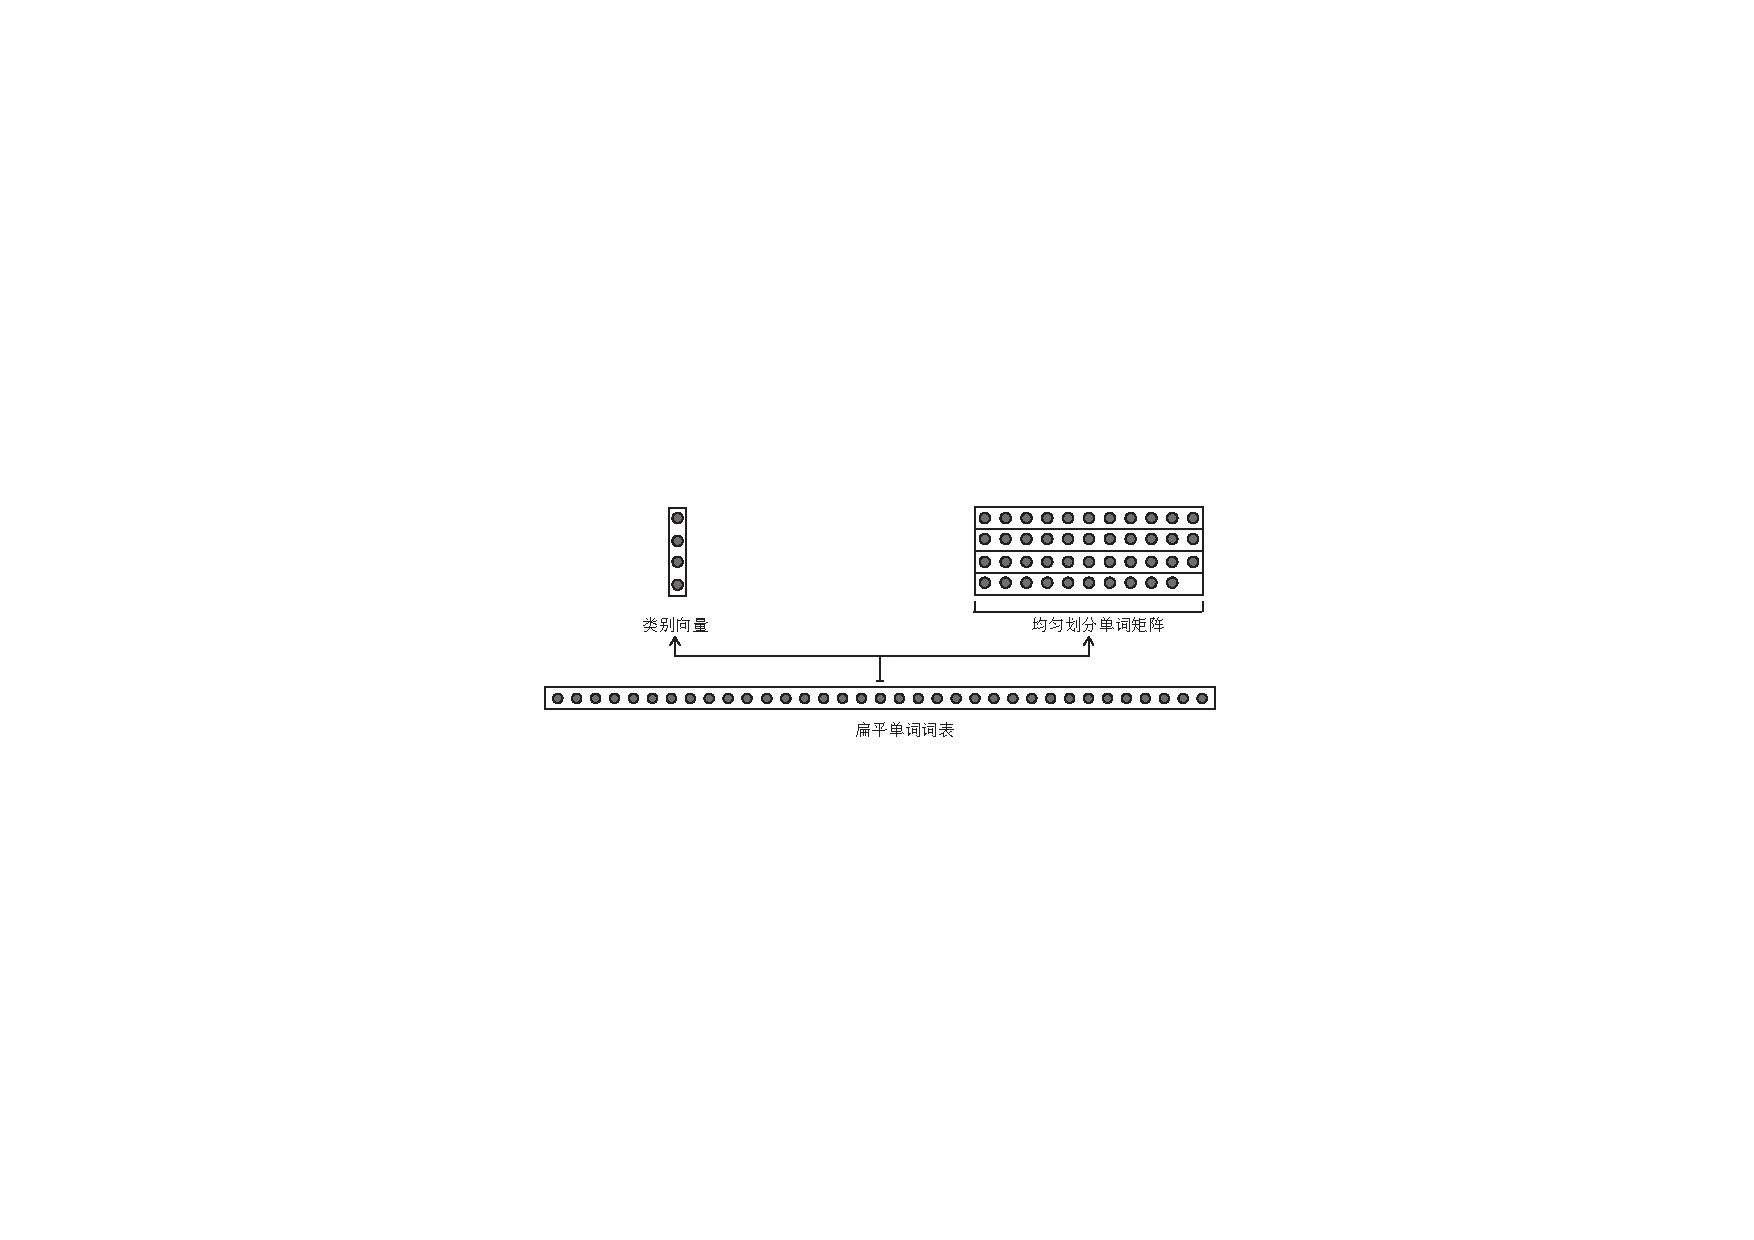
\includegraphics[width=.9\linewidth]{./figures/chsm-simple2.pdf}
\caption{均匀词表划分结构示意图}\label{fig:equal}
\end{figure}

上述的编码方式将一维~1-of-K~的单词索引替换成元组方式的索引~$(w^c,w^o)$,通过该元组可以从预先定预先定义的单词查找表~$\Gamma $~中检索给定单词~$w$,或者给定单词~$w$,通过反向的查找表给出该元组。其中~$w^c$~指代的是单词的类别编号,$w^c$~表示该组内的单词索引。这种编码方式不仅能处理传统的均匀划分词表同时也支持非均匀划分的词表结构。


\section{基于类别的代价函数和导数}
在定义单词基于类别的二元编码后,本章接下来讨论基于这种编码的代价函数和导数计算公式。
给定隐藏层输出向量~$h$,那么该分组中的每个组和和该分组中单词的局部概率可以被定义为:
\begin{equation}
\setlength{\abovedisplayskip}{10pt}
\setlength{\belowdisplayskip}{10pt}
\begin{split}
\log p^c(c|h) &= \theta^c h-\log \sum{\exp( \theta^c h )} \\
\log p^o(w|w^c,h)&=\theta^o h -\log\sum\exp{(\theta^o h)}
\end{split}
\end{equation}
其中~$p^c$~和~$p^o$~是分别计算而不是同时计算的。因为主要的计算瓶颈在单词局部概率~$p^o$~中,所以主要问题是减少第二项概率的计算量而不是同时计算这两项概率。因此本文的主要工作集中在如何高效计算~$p^o$。例如,假设我们将词表大小为~10000~的单词均匀划分,那么类别向量的维度是~100,单词矩阵的维度是~$[100,100]$。如果两者能够同时计算,而不是依次计算,它所带来的计算效率增益可以如下计算:
\begin{equation}\label{equ:example}
\setlength{\abovedisplayskip}{10pt}
\setlength{\belowdisplayskip}{10pt}
  \frac{\frac{1}{100*100}}{\frac{1}{100*100+100}}-1=1\%
\end{equation}
从上面的计算结果来看,我们只能提升~$1/\%$~的速度方面性能。那么如果每次只计算对应单词的单词矩阵的概率值,计算效率可以如下计算:
\begin{equation}\label{equ:example2}
\setlength{\abovedisplayskip}{10pt}
\setlength{\belowdisplayskip}{10pt}
  \frac{\frac{1}{100+100}}{\frac{1}{100*100+100}}-1=49.5
\end{equation}
可以发现,只要能避免计算全局概率就能实现~$49.5$~倍的计算效率增益。使用分类的层次概率模型能直接将模型的计算瓶颈削弱到很少计算时间,尽管相比于树状模型该模型的计算速度不是最快的。除此之外,基于类别的层次概率模型的优点包括:1)模型鲁棒性更强,单词的分组分布对模型的精确度影响比树状层次概率模型小;2)模型实现容易,通用性强。只需要将所有单词划分几个分组即可,不需要做层次二叉聚类算法,而且层次二叉聚类算法计算时间复杂度相当高,不适合实际使用。



在介绍完模型的类别编码方式中提及的掩码向量并不是直接应用于这个分词矩阵,而是应用在对数概率归一化(log softmax)的计算步骤中。 举例来说,在~softmax~函数中:$p(x_i)={\exp({x_i}})/{\sum_j\exp(x_j)}$,如果~$x_k=0$,然而其概率值~$p(x_k)>0$~,这是因为~$\exp(x_k)>0$。即:在该类别中不存在的单词,仍然有概率数值和概率分布,这样对于那些实际存在的单词概率来说,至多有~$\mathcal{|V|/\mathcal{C}}-1$~的类别概率被稀释,这被称为概率稀释问题。因此,该组中正确的的局部单词的对数概率计算如下:
\begin{equation}
\setlength{\abovedisplayskip}{10pt}
\setlength{\belowdisplayskip}{10pt}
  \log \tilde p^o(w|w^c,h)=\theta^o h -\log\sum\theta^m\exp(\theta^o h)
\end{equation}
其中~$\theta^m\exp(\theta^o h)$~保证了那些不存在的单词经过掩码向量之后数值是~0,从而不会对公示的第二项产生影响。

接下来推导模型的代价函数,模型的预测损失主要来自两项:类别预测错误和分组中的单词预测错误,所以该层次模型的损失函数可以从这两项错误分类中算出,可以写成如下的形式:
\begin{equation}
\setlength{\abovedisplayskip}{10pt}
\setlength{\belowdisplayskip}{10pt}
\ell(\theta|h) =\log p^c(w^c|h) +\log \tilde  p^o(w^o|w^c,h)
\end{equation}
其中计算$\log \tilde  p^o(w^o|w^c,h)$,需要指定其类别~$w^c$。在模型训练过程中,$w^c$~是需要预先定义的,在测试过程中,需要同时考虑 ~$p^c$~和 ~$p^o$~两项概率,才能选择概率最大的单词,单独计算$\arg\max p^c$~和 ~$\arg\max p^o$~均无法获得概率最大的单词。

总的来说,将词表分成相互排斥的分组的优点可以概括为:1)避免了在整个词表上计算归一化(Normalization)概率。 由于~$p^c$~是在类维度上计算概率归一化概率,$p^o$~是在最大组大小维度上计算归一化概率。 所以在第二个方程中,其他分组中的单词被忽略不需要计算,其中~$\mathcal{|C|}$~和~$\mathcal{|V|}/\mathcal{|C|}$~在最大的实验数据集都不会超过~1000; 2)与基于二叉树结构相比,它对词表的结构约束(Structural Constraint)更少,在分层预测过程中丢失的信息更少;3)与单词拆分方法相比,它不会增加序列长度,所以不会影响循环网络的长距离依赖的建模问题。

当定义模型的代价函数之后,接下来推导得模型所涉及的参数的导数,以便于模型求解优化。模型的所有的参数包括:$\{\theta^c,\theta^o,h\}$,模型的代价函数对于这些参数的导数计算公式如下:
\begin{equation}
\setlength{\abovedisplayskip}{10pt}
\begin{split}
\frac{\partial \ell}{\partial \theta^c}=& (\delta_{ij}-p(c|h))h \\
\frac{\partial \ell}{\partial \theta^o}=&(\delta_{ij}-p(w|c,h))h \\
\frac{\partial \ell}{\partial h}=&(\delta_{ij}-p^c(c|h))\theta^c + (\delta_{ij}-p^o(w|c,h))\theta^o
\end{split}
\end{equation}


\section{基于类别的测试推理}
在推理测试阶段,对于类别的层次概率模型来说,序列的概率直接运用模型的代价函数计算获得,如下所示:
\begin{equation}\label{equ:class_inf}
\setlength{\abovedisplayskip}{10pt}
\setlength{\belowdisplayskip}{10pt}
\log p(w_1,\cdots, w_T)=\sum_t^T\log p(w_t|h_t) =\sum_{t=1}^{T}\log p^c(w^c_t|h_t) +\log p^o(w^o_t|w^c_t,h_t)
\end{equation}
其计算复杂度是~$\mathcal{O(|H|\sqrt{|\mathcal{V}|})}$~,比softmax函数计算效率更高,两者的加速比是~$|\mathcal{V}|/\sqrt{|\mathcal{V}|}$。

\begin{algorithm}[!ht]
\caption{基于 cHSM 算法的全局 $\arg\max$ 算法}\label{algo:alls}
\KwData{ 隐藏层输出 $h$}
 \For{$c \in \mathcal{C}$ }{
 {// 计算类别的概率~$\log p^c(c|h)$}\;
 {$\log p^c(c|h) = \theta^c h-\log \sum{\exp( \theta^c h )}$}\;
 \For{w $\in$ c}{
 {// 计算单词的条件概率~$\log p^o(\hat w^o|\hat y^c,h)$}\;
 {$ \log \tilde p^o(w|w^c,h)=\theta^o h -\log\sum\theta^m\exp(\theta^o h)$}\;
 {// 计算每个单词全局概率}\;
  {$\log p(w|h)=\log p^c(w^c|h)+\log \tilde p^o(\hat w^o|\hat w^c,h)$}\;
 }
 }
 {$w=\arg\max_w \log p(w|h)$}\;
 \KwResult{概率最大的候选单词$w$。}
\end{algorithm}

其次对于第二种词表排序的情况,首先可以计算词汇表中所有单词的概率,然后调用排序函数,从而选择概率最高的单词,如算法~\ref{algo:alls}~所示。 此外,我们仍然可以在算法~\ref{alog:exact}~中对上述方法进行少量修改,然后计算全局概率最佳的单词。两者的差异是,算法~\ref{alog:exact}~最后的$\arg\max$的计算量是~$\mathcal{|C|}$,算法~\ref{algo:alls}~最后的$\arg\max$的计算量是~$\mathcal{|V|}$。
\begin{algorithm}[!t]
\caption{基于~cHSM~算法的贪心$\arg\max$ 算法}\label{alog:exact}
\KwData{ 隐藏层输出 $h$}
{// 挑选每个类中概率最大的单词}\;
 {$\hat w^o=\arg\max_o{\log p^o(w| c,h)}$ }\;
 {// 在这些已经被栅选单词中挑选最佳的单词}
 {$\tilde w^c=\arg\max_c{\log p^c(w^c|h)+\log p^o(\hat w^o|\hat y^c,h)}$}\;
通过查找表 $\Gamma'$ 将 $(\tilde w^c,\hat w^o[\tilde w^c])$替换成单词$w$ \;
 \KwResult{概率最大的候选单词$w$。}
\end{algorithm}


此外,cHSM算法的性能对词表划分算法有些敏感,因为某些方法可能会产生高度不平衡的字组,并且这种单词不均匀分布会在算法中产生标签偏差问题(Label Bias)。第一个本地~$\arg\max_o$~进程~\upcite{DBLP:conf/icml/LaffertyMP01}。然而,在大多数情况下,如果选择合适的参数,则可以考虑不平衡的问题,本文考虑平衡词汇分区的广义形式。

我们接下来来详细说明标签偏差问题。考虑两个类~$c_p$~和~$c_q$,这两个类的包含的单词数量是不同的,我们不妨假设~$|c_p|\le|c_q|$。在计算了最后一个隐藏层输出~$h$~与类图层参数的相似性之后,我们继续计算~$h$~与每个组的内部单词~$w$ 的相似性得分,这些单词在每个特定组中都没有进行局部规范化整个词汇。当~$|c_p|\approx|c_q|$~表示我们希望将词汇聚类成等大小的群组,而不是高度倾斜的群组分布时,可以减轻标签偏差问题,其中~$|c_p|\ll|c_q|$ 。更具体地说,对于分布不均的情况,对于类~$c_q$~中的单词来说这个概率被一大群单词稀释是不公平的,这样算法更有可能以较高的概率取出这个小组中的单词,放弃在其他大集团有更多的潜在的话。

我们可以用局部贪心算法搜索次优结果,而不是搜索确切的全局最优结果,可以将这个$\arg\max$进程分解为两个阶段:1)计算类概率,并挑选概率最大的类 $\hat c $; 2)计算该类别下的单词概率 $\hat c$,并选择具有最高局部概率的单词。这个算法会给出局部最优的单词而不是全局最优的单词,但是与原始算法~\ref{alog:exact}~相比,它的运行速度要快得多。而且,由于单词计算的是局部概率归一化,标签偏差问题可以在一定程度上缓解。在实验研究中将讨论算法~\ref{alog:exact}~和~\ref{alog:cargmax}~的详细不同性能。
\begin{algorithm}[!t]
 \caption{基于 cHSM 模型伪贪心 $\arg\max$ 算法}\label{alog:cargmax}
\KwData{隐藏层输出 $h$;}
{// 挑选概率最大的类别}\;
 {$\hat w^c=\arg\max_c{\log p^c(c|h)}$ }\;
 {$\hat w^o=\arg\max_o{\log p^o(w|\hat w^c,h)}$}\;
 {// 在这个类别下面,挑选概率最大的单词}\;
 {通过查找表 $\Gamma'$ 将 $(\hat w^c,\hat w^o)$替换成单词$w$}\;
 \KwResult{ 最佳的候选单词 $\hat w$.}
\end{algorithm}

\section{词表划分算法}
由于cHSM模型的性能与其词汇分割算法密切相关,我们将聚类算法的现有工作进行汇总,并将可能的方法分类如下:

\subsection{均匀词表划分算法}
1) 随机初始化。 这种直观的方法忽略了单词的所有外部信息,能用于揭示其他聚类方法的最坏情况,也可以揭示其他聚类策略的相对收益。

2) 字母顺序。这种方法根据字符级别的信息对单词进行排序,同一组中的单词共享一个相似的子字符串。


3) 一元单词聚类。这些单词首先根据它们在文本中的频率排序,然后对这个列表均匀划分,从而形成词频连续的单词块。这种方法具有这样的性质:编号较低的类比较高编号的类访问频率更高,因为它们的词频更高~\upcite{DBLP:conf/nips/MikolovSCCD13}。



\subsection{非均匀词表划分算法}
1) 二元单词聚类。又称为指布朗聚类方法,这是历史适用于基于N-gram的基于类的模型~\upcite{DBLP:journals/coling/BrownPdLM92,liang2005semi}。单词使用相同的Bi-gram信息将会划分到相同的行中。

2) 结构聚类\footnote{https://github.com/AlonDaks/unsupervised-authorial-clustering}。根据文本中的单词的词性和句法结构划分词表~\upcite{DBLP:conf/acl/DaksC16} 。

3) 语义聚类。我们将传统的kmeans聚类方法应用到预训练的词响亮,使得我们可以通过指定聚类的大小将词汇分成不同的形状。

\section{本章小结}
本章首先定义了基于词表划分的编码概念,同时给出了模型所涉及的参数的详细含义。接下来,为了支持词表的非均匀划分结构,我们提出了二元组的编码方式,将非均匀单词矩阵填补成均匀矩阵和对应的掩码矩阵,然后逐步推导模型的概率公式和代价函数。进一步的,我们还讨论了模型在测试的时候所需的推理算法,因为基于划分词表的概率计算方案和传统的softmax计算方案不同,不能直接输出单个词的概率或者计算最佳的候选单词,所以我们分别针对这两个任务提出推理算法。最后,由于单词在单词划分矩阵上的分布需要初始化,我们讨论了传统的霍夫曼硬聚类算法,布朗软聚类算法和语义向量软聚类算法等等。同时也讨论三种算法的实际应用过程。

\chapter{语言模型实验结果与分析}
在前面两章中,我们分别介绍了树状分层概率计算模型和类别层次概率计算模型的具体建模过程。在本章中,为了比较所提出的分层并行概率计算模型与已有的计算模型方法(Baselines)的效率和准确性,我们将在三个标准文本数据集:Wikitext-2,Wikitext-103 和 One Billion Word数据集上,进行了循环语言建模任务的实验研究和实验结果分析。本文将会展示并行层次概率计算算法的实验结果,我们还会与其他大词表问题的优化加速算法相互对比。 此外,我们还将从效率分析、可扩展性、参数大小和性能等四个方面,对这些已有的方法进行实验研究并作讨论分析。

\section{实验设置}
在这一小节,我们将介绍实验所需要用到的文本数据集,语言模型实验的两种主要的评测指标和实验模型的实际训练参数配置和训练过程。
\subsection{实验数据集}
本次实验所采用的数据集主要是依照两个目的选取的:我们需要在小数据集能反映参数变化对模型的最后的效果产生的影响,同时我们还需要大数据集展示模型参数在最佳配置下模型的最优结果比较情况。所以在本次实验中,我们选取了三个标准文本数据集:Wikitext-2,Wikitext-103 和 One Billion Word数据集。
如表~\ref{tab:dataset}~所示,表中列举了这三个数据集全部统计指标:单词数量、句子数量、词表大小和词表外单词的比例(Out-of-Vocabulary)。这里我们需要注意的是,我们不能改变词表大小,而且不同词表大小的模型之前理论上是没有互相比较的意义的。
因为我们接下来要计算的一个重要的评测指标就是和词表大小成负相关关系的。
所以表~\ref{tab:dataset}~中展示的数据已经预先固定了,不会再做任何的修改,例如:单词大小写变化,数词转换操作或者分词操作。
\begin{table}
  \centering
  \caption{WikiText-2, WikiText-103 和 One Billion Words 数据集统计指标 \label{tab:dataset}}
\begin{tabular}{llrrrrr}
\toprule
数据集& 类型& 文章数 & 句子数量 &  单词数量 &词表大小 & OOV (\%) \\ \midrule
\multirow{3}{*}{Wikitext-2} &训练集& 600 & 36,718 & 2,088,628 & \multirow{3}{*}{33,278} & \multirow{3}{*}{2.6\%} \\
&验证集& 60 &3,760 & 217,646  & &\\
&测试集& 60 & 4,358 & 245,569 & &\\
\midrule
\multirow{3}{*}{Wikitext-103} &训练集& 28,475 &  1,801,350 &  103,227,021 & \multirow{3}{*}{267,735} & \multirow{3}{*}{0.4\%} \\
&验证集& 60 &3,760 & 217,646  & &\\
&测试集& 60 & 4,358 & 245,569 & &\\
\midrule
\multirow{3}{*}{One Billion Word} &训练集& --- &30,301,028&768,646,526&   \multirow{3}{*}{793,471} &   \multirow{3}{*}{0.28\%} \\
 &验证集& --- &  6,075 &   153,583 &&\\
 &测试集 & --- &  6,206 &   159,354 &&\\
\bottomrule
\end{tabular}
\end{table}

其中,对于~Wikitext-2和Wikitext-103~数据集,训练、验证和测试集都是预先划分固定的,并且其词汇表大小也已经被定义\footnote{https://metamind.io/research/the-wikitext-long-term-dependency-language-modeling-dataset/}。
这两个数据集拥有相同的验证和测试集,而Wikitext-103的训练集则比Wikitext-2的训练集大得多。所以我们还可以间接测算出增大训练集对测试集上的提升效果表现。对于第三个``One Billion Word''数据集\footnote{http://www.statmt.org/lm-benchmark/},它是由之前机器翻译数据集里面的的文本融合而成,文本数据也取自维基百科(Wikipedia)\footnote{英文维基百科主页:https://en.wikipedia.org/wiki/Main\_Page/}。
为了评价的标准性和实验的可互相比较性,官方还提供了一套数据预处理脚本,同时指定了该脚本所需要的~Perl~语言版本,可见要求极为严苛。因为对于语言模型来说,Perl~内置函数处理出来的文本也略有不同,语言模型之间的结果相互比较就会变得没有意义的。通常来说,词表小的模型更占优势。当我们用官方提供的脚本处理完数据后,我们将``./train/''目录中的所有数据视为训练集,选择``./holdout/''目录下面的第一和第二个数据集作为相应的验证和测试集。这些数据集的详细统计指标在表~\ref{tab:dataset}~中进行了详细说明。

\subsection{实验评价指标}
在本次实验研究中,当我们将各种实验模型在训练数据集上训练到收敛之后,我们就需要评价不同模型的性能差异,针对语言模型的两个标准评估度量标准来揭示针对不同的优化方法的优劣:困惑度(Perplexity,$ \mathrm{PPL} $)和单词误差率(Word Error Rate,$\mathrm{WER} $)。
其中,$ \mathrm{PPL} $是一个内在度量指标(Intrinsic Metric),代表了在候选人中选择下一个话语时的混乱程度。语言模型较低的困惑意味着在相同词表下拥有更好的可预测性。此外,在整个测试集上,$\mathrm{PPL}$ 数值是与平均负对数似然值(NLL)呈指数相关关系,表示我们训练过程中我们直接优化了我们的评测指标,即困惑度量。
\begin{equation}\label{equ:ppl}
   \mathrm{PPL}(w_1,\cdots,w_T)=\sqrt[T]{\frac{1}{\prod_{t=1}^T p(w_t|w_{1:t-1})}}
\end{equation}

此外,$\mathrm{WER}$指代的是单词的萊文斯坦距离(Levenshtein Distance),于衡量两个字符串参考句子(reference,记作r)和预测句子(hypothesis,记作h)之间的相似度。他是编辑距离的一种衍生出来的类型,它被定义为错误识别的单词(删除,插入,替换)占单词总数的百分比\footnote{https://martin-thoma.com/word-error-rate-calculation}:
\begin{equation}\label{equ:wer}
  \mathrm{WER} = \frac{\text{插入的单词数 + 删除的单词数 + 替换的单词数}}{\text{全部单词数量}}
\end{equation}
其数学形式的定义公式为:
\begin{equation}\label{equ:distance}
d_{r,h}(i,j) =  \begin{cases}
\max (i,j)& \text{如果}\min(i,j)=0\\
\min  \begin{cases}
d_{r,h}(i - 1,j) + 1,\text{//插入的单词}\\
d_{r,h}(i,j - 1) + 1,\text{//删除的单词}\\
d_{r,h}(i - 1,j - 1) + I{(r_i\neq h_j)},\text{//替换的单词}
\end{cases} &\text{否则}
\end{cases}
\end{equation}
其中$I{(r_i\neq h_j)}$ 指代的是示性函数, 当且仅当$r_i= h_j$的时候取值为$0$,否则该函数取值为$1$。 $d_{r,h}(i,j)$ 表示的是参考句子 $r$的第一个$i$个字符与预测句子 $r$的第一个$j$个字符之间的距离。

我们在本实验中采用萊文斯坦距离作为我们的一个度量指标,主要是考虑到该距离度量的延展性(三角不等式)。 两个字符串的距离不大于分别与第三个字符串的距离之和:
\begin{equation}
d_{r,h}+d_{r,s}\ge d_{r,s}
\end{equation}
其中 $s$ 代表另外一个生成的句子,$d_{r,h}$表示的是句子~r~和句子~h~之间的编辑距离。

除了以上的定量的度量指标,\textit{训练时间效率,词汇可伸缩性}和\textit{运行时内存消耗}等定性度量指标也应该被视为衡量不同模型的重要衡量维度。因此,我们在实验中分别从GPU和CPU的理论和经验角度分析了不同优化算法在不同评估指标上的具体数值结果。最后,统计实验数值并分析在三个标准文本数据集上的最终结果。

\subsection{模型训练和参数配置}
接下来我们来介绍实验模型的参数设置和训练方法。在我们的实验研究中,每个模型都是使用Theano框架实现的而且都运行在一个独立的GPU设备上,它具有12GB的显存(即Nvidia K40m),使得大矩阵乘法的运算成为可能,也就是说我们能测试大词表的计算代价。然而,我们在实际试验中发现随着参数维数的增加,一个GPU显存资源被快速利用殆尽。

然后,对于wikitext-2数据集来说,我们固定最大句子长度为256;对于wikitext-103数据集来说,我们固定最大句子长度为100;对于OBW数据集来说,我们固定最大句子长度为50,因为它词表最大,需要占用更多的显存消耗。对于长度超过长度阈值的那部分字符串,超出部分全部删除。由于我们测量的是语言模型的单词级损失(Word-Level Loss)而不是句子级的分数(Sentence-Level Loss),因此删除部分的那句子对模型训练的影响是很小的。
\begin{figure}[!t]
  \centering
  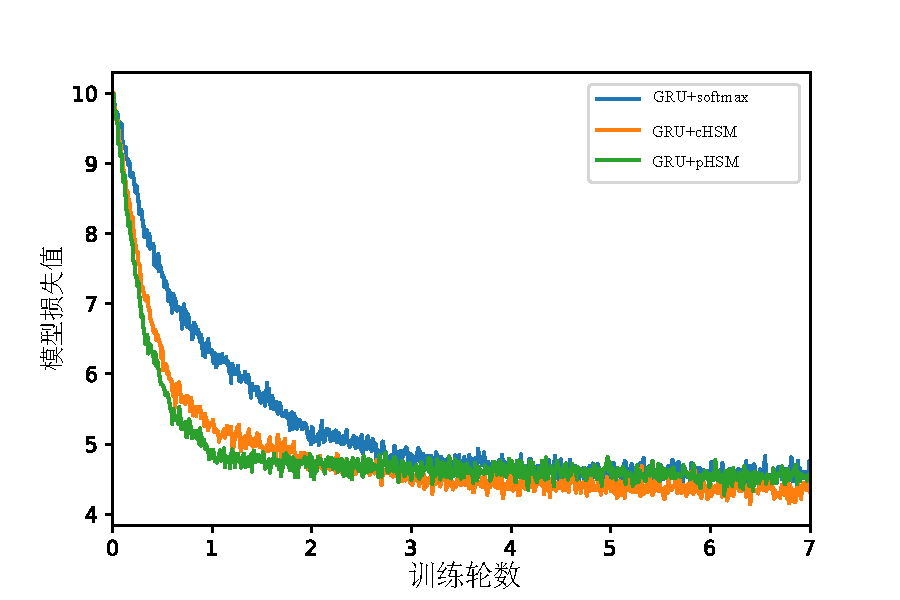
\includegraphics[width=0.6\columnwidth]{./figures/learn2.pdf}
  \caption{模型训练曲线图}
\end{figure}

另外,我们实验中采用Adam优化器(Optimizer)配合两种不同的学习率(Learning Rate),即设置$ lr = 0.06$ 和 $0.001 $。对于两种词表层级分解方法,我们将应用较大的学习率;而对于传统的softmax和采样近似方法,我们应用较小的学习率。因为我们实验中发现,词表层级分解算法收敛地很慢,需要配合更大的学习率。除此以外,每隔一定步数,我们还需要衰减学习率的大小:$lr \leftarrow lr *0.9$。

对于在WikiText-2数据集上运行的实验,我们在批处理大小(batch size)为20的20个时期内运行,直到我们观察到验证集上的最小$ \mathrm{PPL} $。验证集上的损失数值约4.8,这是最好的验证上的损失值。而对于Wikitext-103数据集,在训练集上优化参数需要大约3-4个轮数(Epochs),因为训练集大约比较小的一个大50倍。此外,训练集损失数值大约在5.1左右,因为在 wikitext-2 数据集上更高的原因是我们预测的词汇量要大得多,所以混淆程度(即训练损失)应该更高。虽然我们发现模型可以很容易地收敛到局部最小点,验证误差在这个局部最小值的范围内振荡,但是Wikitext-2和Wikitext-103的唯一区别是训练数据的大小,表示收集很多训练数据不一定能保证模型在相同的验证和测试集上学得更好,而不是更普遍的结果。

此外,我们在实验中发现在 OBW 数据集上运行实验相当具有挑战性,因为它需要更大的参数来拟合。所以我们应用优化的CUDA实现的RNN模型~\upcite{DBLP:journals/corr/AppleyardKB16},将RNN模块所需要的计算时间降到最低。然而,等待模型收敛到训练集上需要480小时,因此我们可以在验证集上得到可能的结果。

\section{影响因素比较}
我们在这部分将讨论语言模型的大词表问题的具体实验计算瓶颈和各种不同计算策略对实验计算效率和性能的影响。
\subsection{词表层次化比较}
我们首先使用wiki103数据集,统计了语言模型中每个模块的计算时间消耗,如图~\ref{fig:rnn_timing}~所示。 我们计算运行不同的RNN模型(即LSTM模型和GRU模型)及其梯度(即,RNN Grad)所需的时间,以及Wikitext-103数据集的大词汇表上的常规softmax,这词汇表大小与我们平时所采用的数据集的词表相当。 我们分别用Theano框架和CUDA实现了RNN单元,一个采用python语言实现,第二个使用并行C++语言实现。目前基于CuDNN实现的RNN模型计算时间最快,它里面的RNN的运行时间可以缩短到最短。 我们将代码重复了100遍,统计了每个模块的总时间占用,然后分别计算其平均时间占用。这样做的目的是通过多次实验来保证实验数据准确性。

从图中可以看出,使用优化的CUDA,softmax模块的影响比RNN单元及其梯度更重要。Softmax计算时间占用总计算时间随着词表的增大占比越来越大,并且已经超过了$50\%$的计算时间,这就需要我们详细讨论softmax优化。


\begin{figure}[!t]
  \centering
  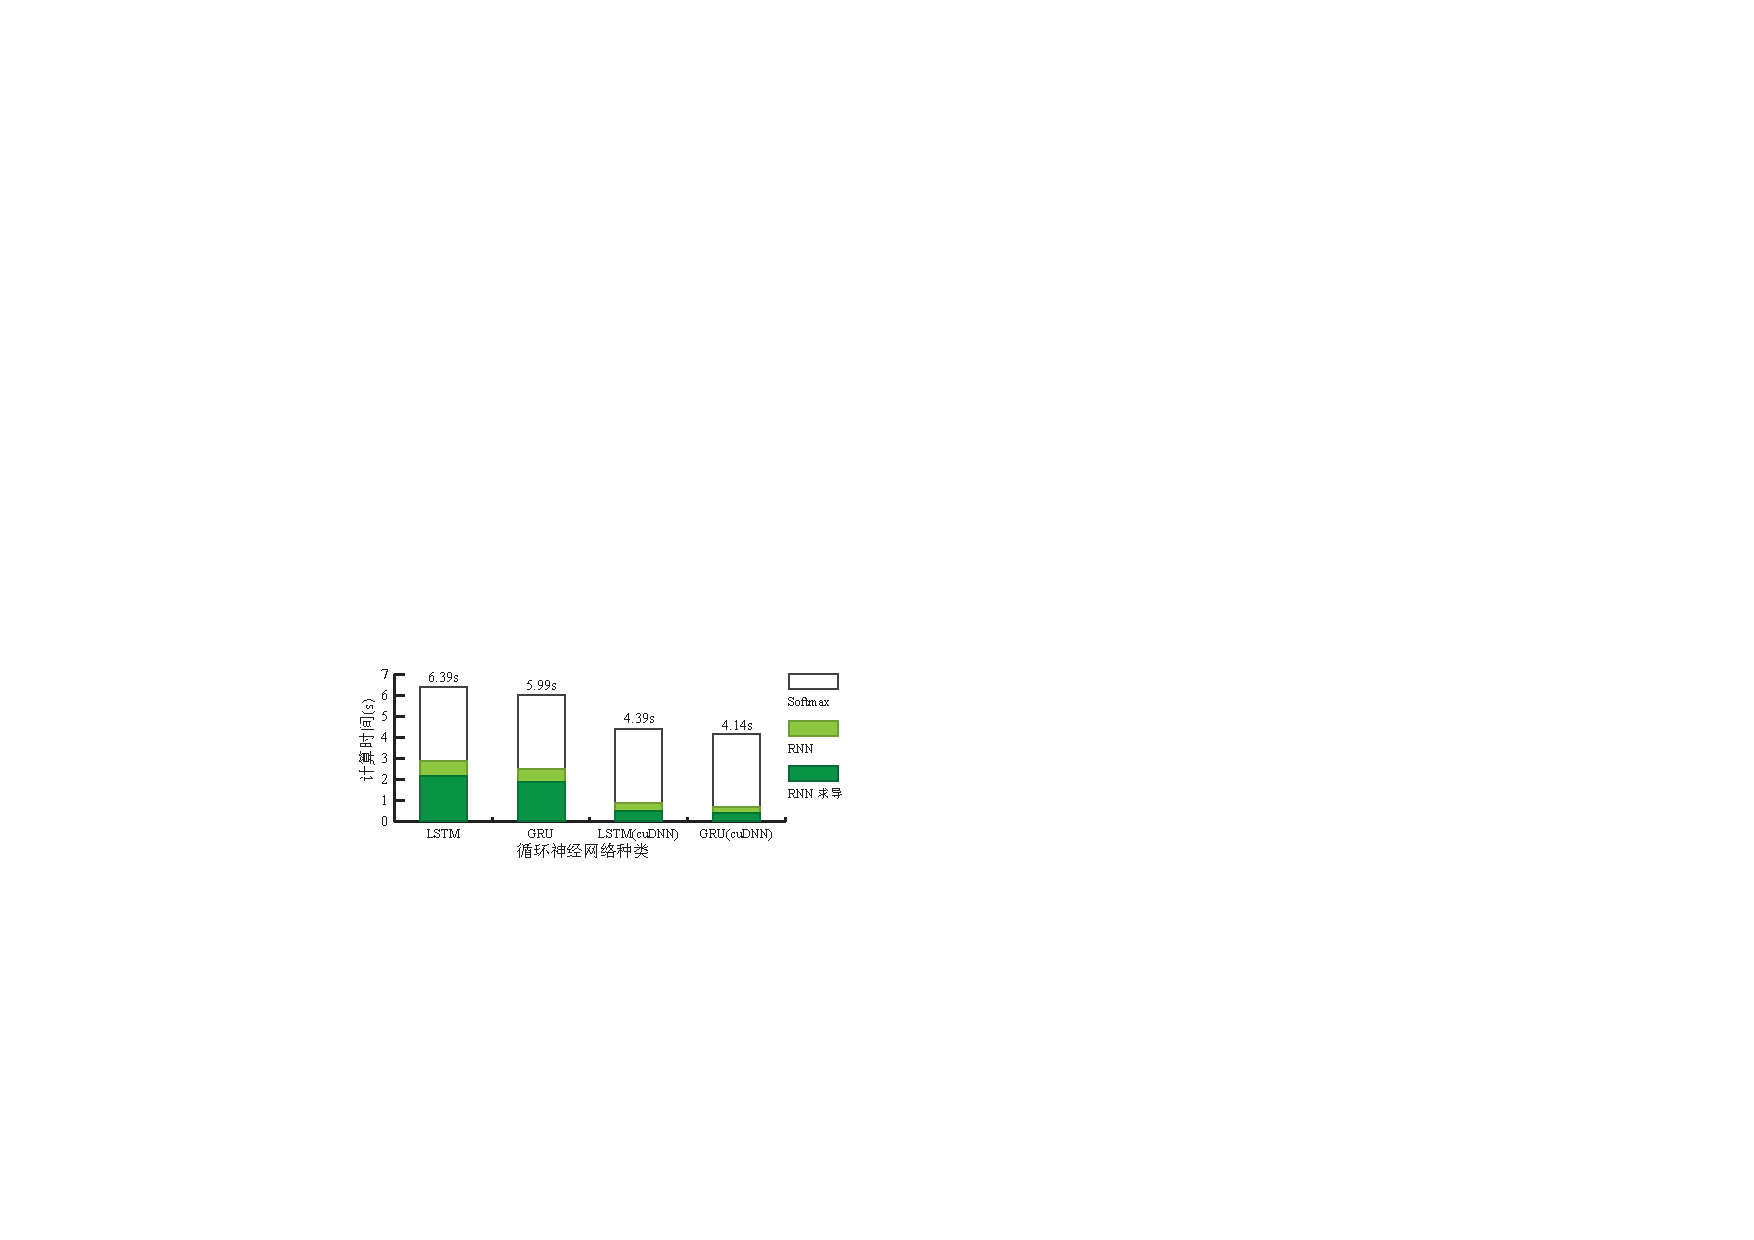
\includegraphics[width=.9\columnwidth]{./figures/rnn_timing.pdf}
  \caption{wikitext-103数据集上测量语言模型三个部分的计算时间比较}\label{fig:rnn_timing}
\end{figure}
\begin{figure}[!t]
  \centering
  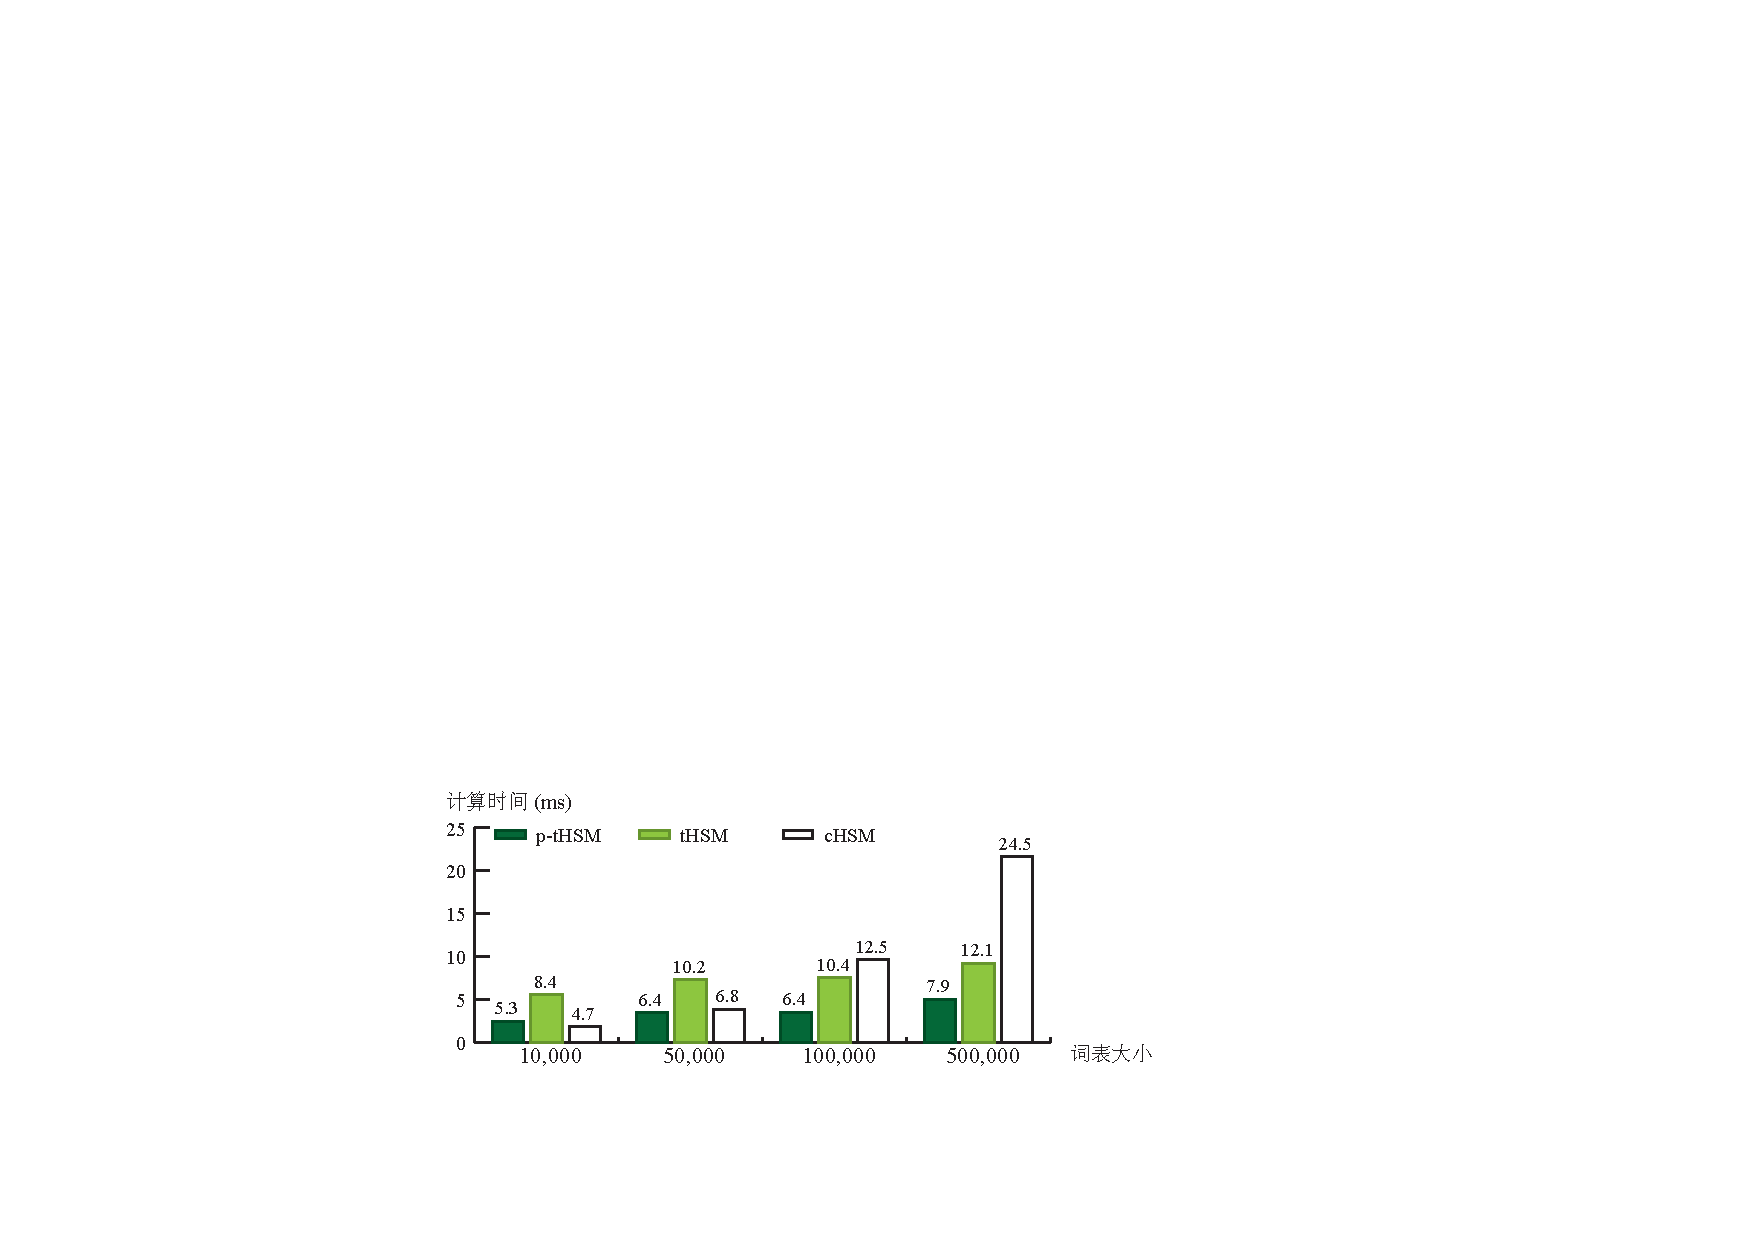
\includegraphics[width=.87\columnwidth]{./figures/all_time.pdf}
  \caption{cHSM, tHSM 和 p-tHSM 算法随着词表大小的计算时间影响}\label{fig:hsm_benchmark}
\end{figure}

为了对用于训练相同批处理数据的经验时间复杂性和内存消耗进行基准测试,我们使用这些算法在表~\ref{tab:time}~中收集了GPU和CPU上的详细结果。我们尝试使用这些算法处理WikiText-103数据集,并计算处理一个批处理数据所需的平均时间。另外,输入句子的最大长度,隐藏层,输出词汇和批量大小分别设置为$\{50, 256, 267735, 20\}$。此外,“总时间”过程表示前向传播和后向梯度优化的过程,“前进时间”过程表示从输入数据到计算模型成本所需的时间消耗。此外,我们计算了上述算法训练期间加载所需的内存。 $ \mathcal{| V |} $表示词汇大小,$ \mathcal{| H |} $是目标嵌入维度。在训练期间,tHSM只消耗最小的存储器资源,而p-tHSM覆盖了更大的存储器集合,并且p-tHSM在考虑存储器消耗和速度时采用更大的存储器并且获得了更好的加速比。

\begin{table}[!ht]
  \centering
  \caption{wikitext-103数据集上面GPU和CPU的运行时内存和计算时间比较\label{tab:time}}
\begin{tabular}{lccccc}
  \toprule
 \multirow{2}{*}{算法}  &\multirow{2}{*}{运行时内存占用} &\multicolumn{2}{c}{总计算时间 (ms)} & \multicolumn{2}{c}{前向计算时间 (ms)}   \\
   \cmidrule(lr){3-4}  \cmidrule(lr){5-6}
	& & CPU&GPU & CPU& GPU \\ \midrule
Softmax & $\mathcal{|HV|}$ &510.4  &262.1&352.2& 62.9 \\
cHSM    & $2\mathcal{|H|\sqrt{|V|}}$&506.5  &\textbf{40.6}&28.7&14.6 \\
tHSM    &$\mathcal{|H|}$&1,004.0 &444.4 & 8.1&  5.6   \\
p-tHSM  &$\mathcal{|H|\log{|V|}}$ &\textbf{383.5}&	86.4 &\textbf{7.0}&	\textbf{1.4} \\
  \bottomrule
\end{tabular}
\end{table}



为了验证与词汇大小相关的cHSM,tHSM和p-tHSM算法的可扩展性,结果展示在图~\ref{fig:hsm_benchmark}~中。 为了显示p-tHSM算法的影响,我们在这里不包含“Softmax”方法,因为与其他算法相比,它消耗了更多的计算时间,无法被放在这个图里面。 很显然,cHSM随着词汇大小的平方根(即,$ \mathcal{O(| H | \sqrt{| V |})} $)进行缩放,而p-tHSM随着词汇大小的增加呈现出稳定的表现。tHSM算法随着此表大小的对数进行变化 (即,$ \mathcal{O(| H | \log{| V |})} $),我们的p-tHSM算法所需要的计算时间词表变大,与tHSM算法的差异越来越大。这一结果证明我们提出的计算模型更加优越。


在这些实验的基础上,我们可以得出结论:所提出的p-tHSM方法胜过历史记录$ \mathcal{O(| H | \log| V |)})$,并且取得了令人满意的分层softmax方法的加速比。 这种性能归因于基于GPU并行性的加速,也是由于p-tHSM 方法的基本结构,能够将目标字树进行并行地计算。


\subsection{搜索策略的影响}
由于我们提出了三个关于推理阶段搜索策略的算法,其影响可以通过WER度量来观察。在这个结构化预测过程中,一个合适的搜索规则将帮助模型获得最小风险的最佳候选人,如表~\ref{tab:search}~所示。 “Global”方法表示我们计算所有单词的得分,单词的概率用整个词汇全局归一化。值得注意的是,对于cHSM方法算法~\ref{alog:greed_argmax}~比算法~\ref{alog:exact}~得到更好的WER,尽管后一种方法获得了词汇表上的确切顶级候选。由于类结构中存在标签偏差问题,排名最高的词容易出现算法模型无法建模的小组。最后但并非最不重要的是,算法~\ref{alog:exact}~和``global''获得相同的单词排序,唯一的区别是算法~\ref{alog:exact}~避免了冗余计算。所以他们达到了可比的WER得分,但算法~\ref{alog:exact}~需要更少的时间。
\begin{table}[!t]
  \centering
  \caption{wikitext-2数据集上ctHSM算法针对不同搜索算法的WER评测结果\label{tab:search}}
\begin{tabular}{llccc}
  \toprule
   & 算法&计算时间 (ms)&验证集 (WER)& 测试集(WER)\\ \midrule
  \multirow{3}{*}{cHSM} &global&102& 80.00\%& 80.02\%\\
        &算法~\ref{alog:exact}&63& 80.00\%& 80.02\%\\
        &算法~\ref{alog:greed_argmax}&\textbf{44}&\textbf{ 77.09\%}&\textbf{ 77.07\%}\\
  \bottomrule
\end{tabular}
\end{table}

\begin{table}[!t]
  \centering
  \caption{wikitext-2数据集上p-tHSM算法针对不同搜索算法的WER评测结果\label{tab:psearch2}}
\begin{tabular}{llccc}
  \toprule
        & 算法&计算时间 (ms)&验证集 (WER)& 测试集(WER)\\ \midrule
  \multirow{2}{*}{p-tHSM}  &global&161& \textbf{76.67\%}&\textbf{75.35\%}\\
        &算法~\ref{alog:greed_argmax}&\textbf{30} & 79.61\%&79.32\%\\
  \bottomrule
\end{tabular}
\end{table}

对于p-tHSM系列算法,我们比较了所提出的算法~\ref{alog:greed_argmax}和传统的“全局”算法。算法~\ref{alog:greed_argmax}比“global”方法获得本地最佳结果花费的时间更少。由于基于树的模型在以前的决策中更容易失败,所以“全局”方法的MER分数要比算法~\ref{alog:greed_argmax}要好。

\subsection{循环网络模型的影响}

从表~\ref{tab:rnn}~中可以看出,门控单元(即LSTM和GRU单元)的RNN模型在复杂度和字误码率方面比传统的RNN Relu和RNN Tanh模型表现得更好。因为门控功能可以避免梯度消失的问题。虽然它需要稍微多一些的时间进行计算。此外,LSTM的计算公式在GPU上比GRU单元更容易并行运行,因此LSTM比GRU模型需要更少的推理时间。
\begin{table}[!t]
  \centering
  \caption{wikitext-2数据集上不同循环网络针对 PPL、 WER和计算时间的影响\label{tab:rnn}}
\begin{tabular}{lccc}
  \toprule
  循环神经网络 & 计算时间 (ms)&验证集(PPL / WER) & 测试集(PPL / WER)\\ \midrule
  1$\times$RNN Relu~\upcite{DBLP:journals/jmlr/GutmannH10} &176.4&260.52 / 80.00\%&238.75 / 80.02\%\\
  1$\times$RNN Tanh~\upcite{DBLP:journals/iclr/JiVSAD15}   &176.2&250.57 / 79.61\%&230.98 / 79.32\%\\
  1$\times$LSTM~\upcite{7508408}                  &\textbf{189.5}&180.98 / 77.16\%&165.60 / 76.67\%\\
  1$\times$GRU~\upcite{DBLP:journals/corr/ChungGCB14}      &191.3&\textbf{179.59 / 77.09\%}&\textbf{165.32 / 77.07\%}\\ \midrule
  2$\times$RNN Relu~\upcite{DBLP:journals/jmlr/GutmannH10} &266.3&190.52 / 73.01\%&198.75 / 73.02\%\\
  2$\times$RNN Tanh~\upcite{DBLP:journals/iclr/JiVSAD15}   &266.3&189.57 / 72.62\%&260.98 / 72.32\%\\
  2$\times$LSTM~\upcite{7508408}                  &\textbf{279.4}&164.98 / 71.17\%&165.60 / 71.67\%\\
  2$\times$GRU~\upcite{DBLP:journals/corr/ChungGCB14}      &281.2&\textbf{158.59 / 70.08\%}&\textbf{155.32 / 70.07\%}\\
  \bottomrule
\end{tabular}
\end{table}

对于传统的RNN模型,通常通过时间反向传播(BPTT)进行训练,梯度计算步骤中的努力花费在该训练批次中最长序列的长度上是线性的。因此,小批量生产可能效率低下,因为批次中的次序可能有不同的长度。这个问题的一个经典的解决方案是Truncated-BPTT,因此RNN模型的梯度在截断长度上是恒定的,并且对于GPU上的小批量处理是高效的。而前向概率计算步骤仍然是相同的,唯一的影响是避免梯度反向传播步骤。从图中可以看出,较小的截断BPTT在时间效率上取得了较好的效果,较长的截断BPTT长度在PPL度量方面效果更好。
\begin{figure}[!t]
  \centering
  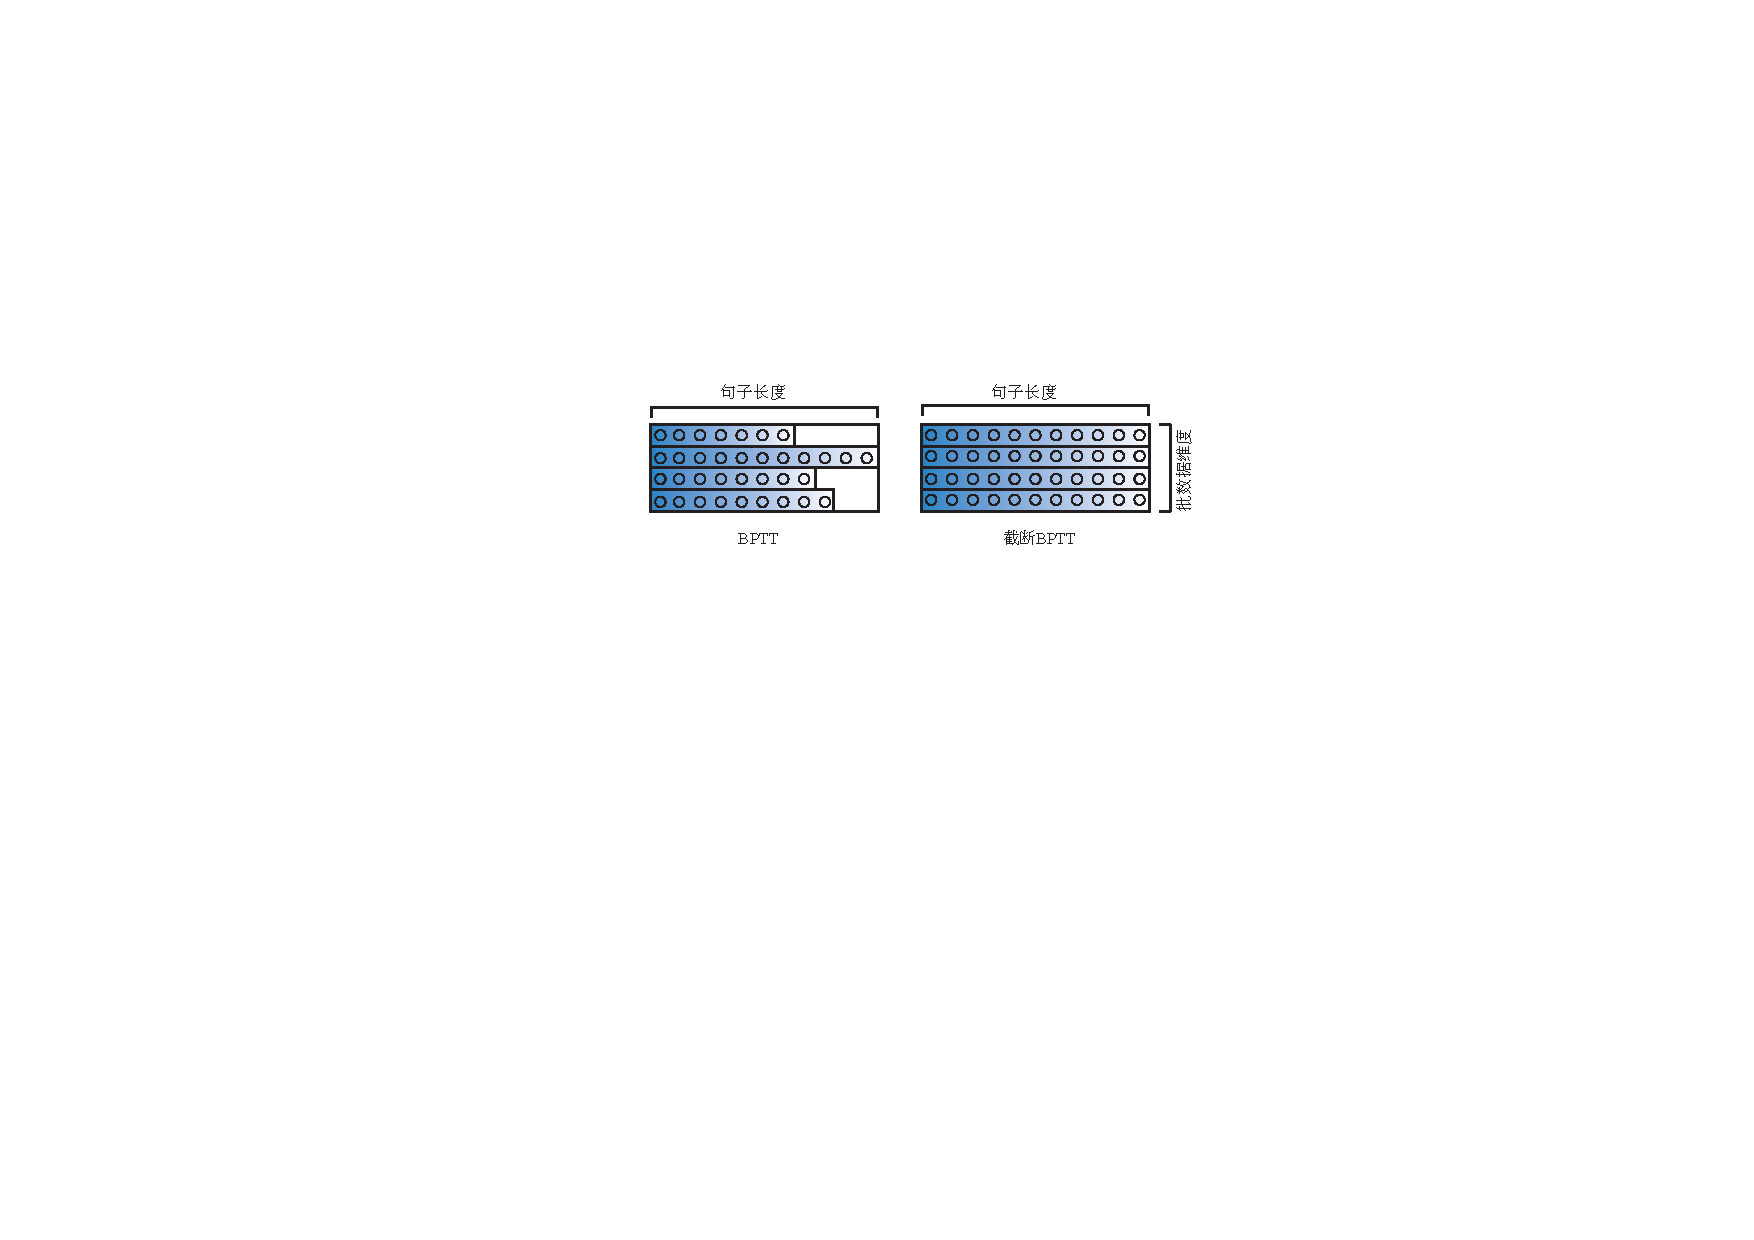
\includegraphics[width=.8\columnwidth]{./figures/minibatch.pdf}
  \caption{BPTT和截断BPTT算法示意图}\label{fig:minibatch}
\end{figure}
\begin{figure}[!t]
  \centering
  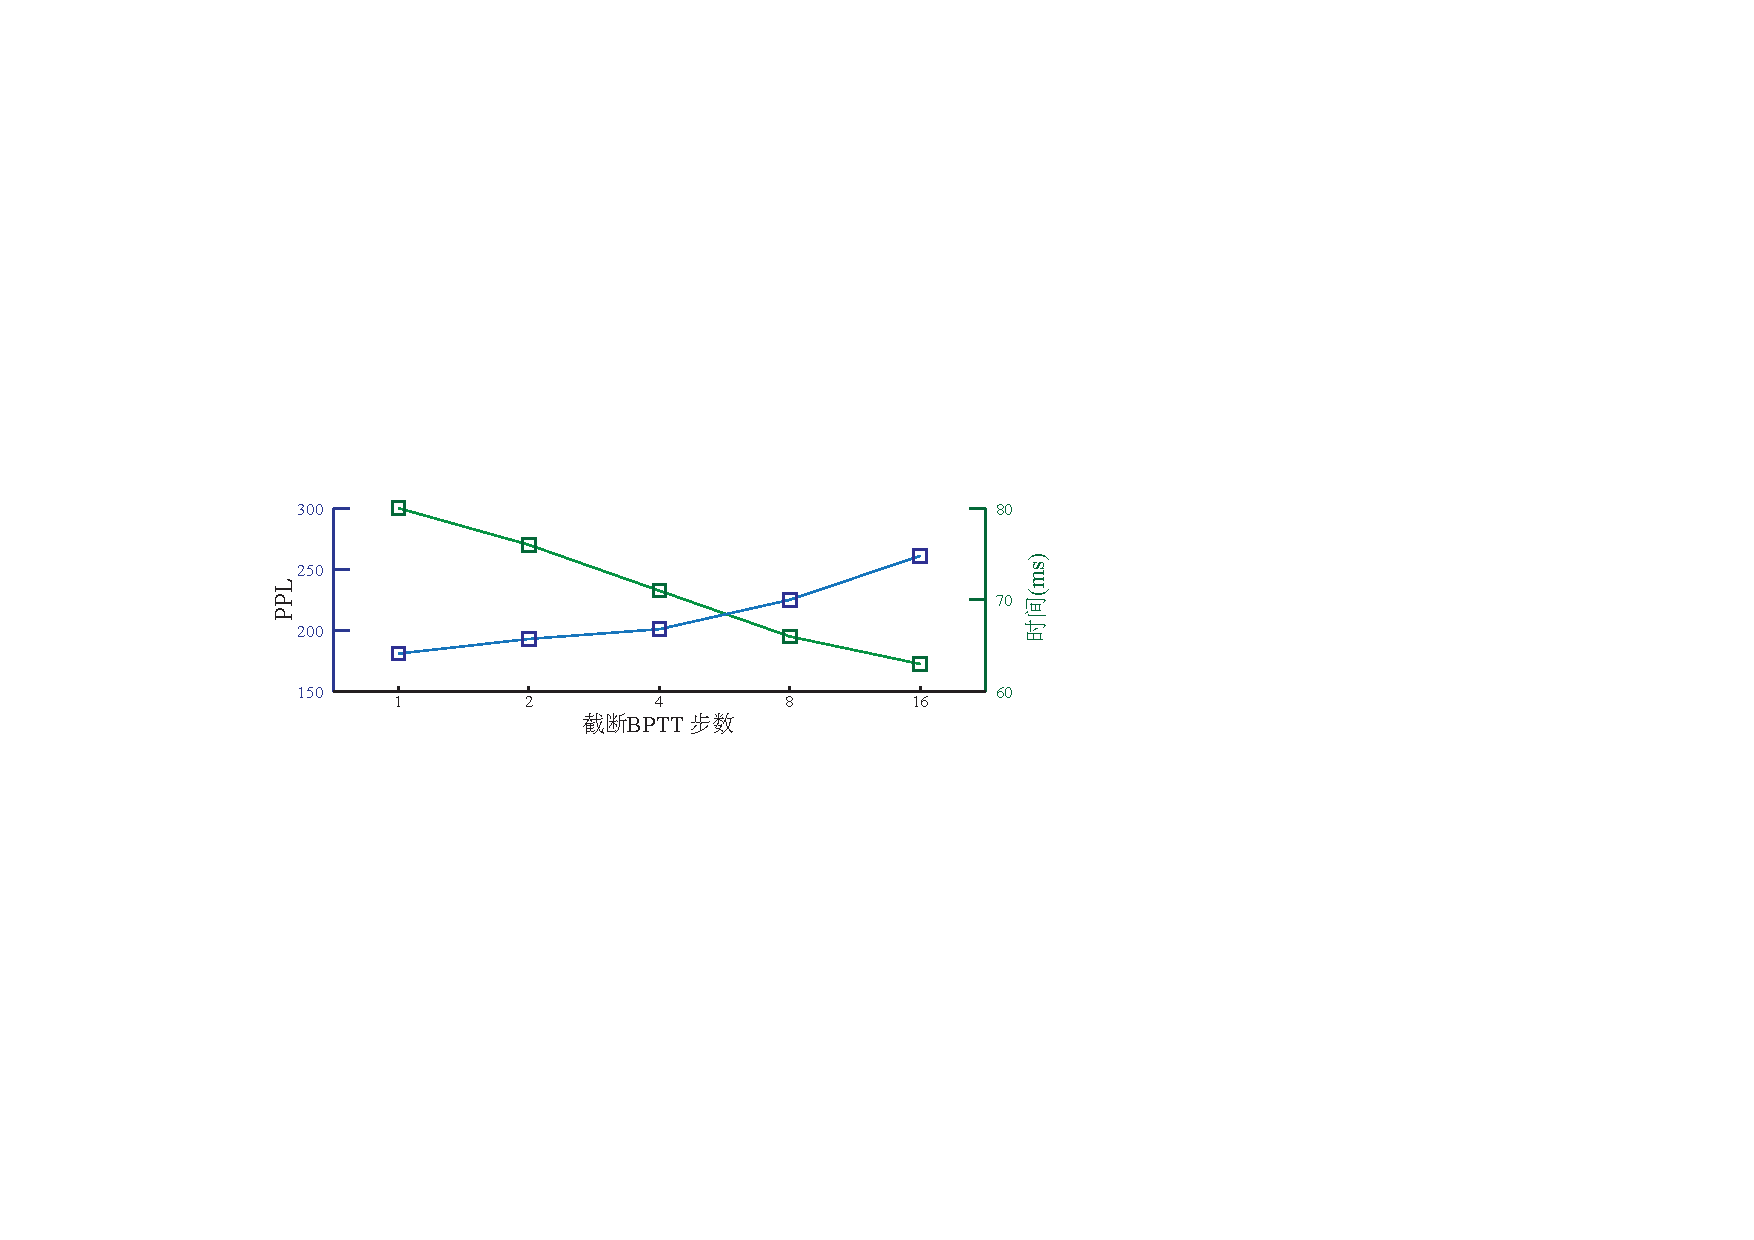
\includegraphics[width=.85\columnwidth]{./figures/tbptt.pdf}
  \caption{wikitext-2数据集上 BPTT和截断BPTT算法对RNN的影响.}\label{fig:tbptt}
\end{figure}
我们在此说明,在训练中,如果你在被截断的段中看到某些依赖关系,则可以学习它们。 如果这些依赖关系总是跨越不同的领域,我们已经打破了这些依赖关系,你永远不会学习它 因为渐变永远不会回流,并告诉前一个段中的某些内容对下一个段是有用的。 但是如果你在一个细分市场中看到他们,那么你实际上有一个希望,那就是在测试的时候,你将能够在不同的细分市场上预测它们。 因为我们总是向前传播。

\subsection{采样近似算法比较}

基于抽样的算法的效率和准确性与样本大小密切相关,我们在下一次评估中测试了这个样本。我们测试了几个样本大小,以评估它们对停电和NCE近似值的影响,结果显示在表~\ref{fig:blackout_nce}中。根据图1所示,中断算法比传统的NCE模型表现得相对较好,这与报道的实验结果是一致的~\cite{DBLP:journals/iclr/JiVSAD15}。

\begin{figure}[!t]
  \centering
  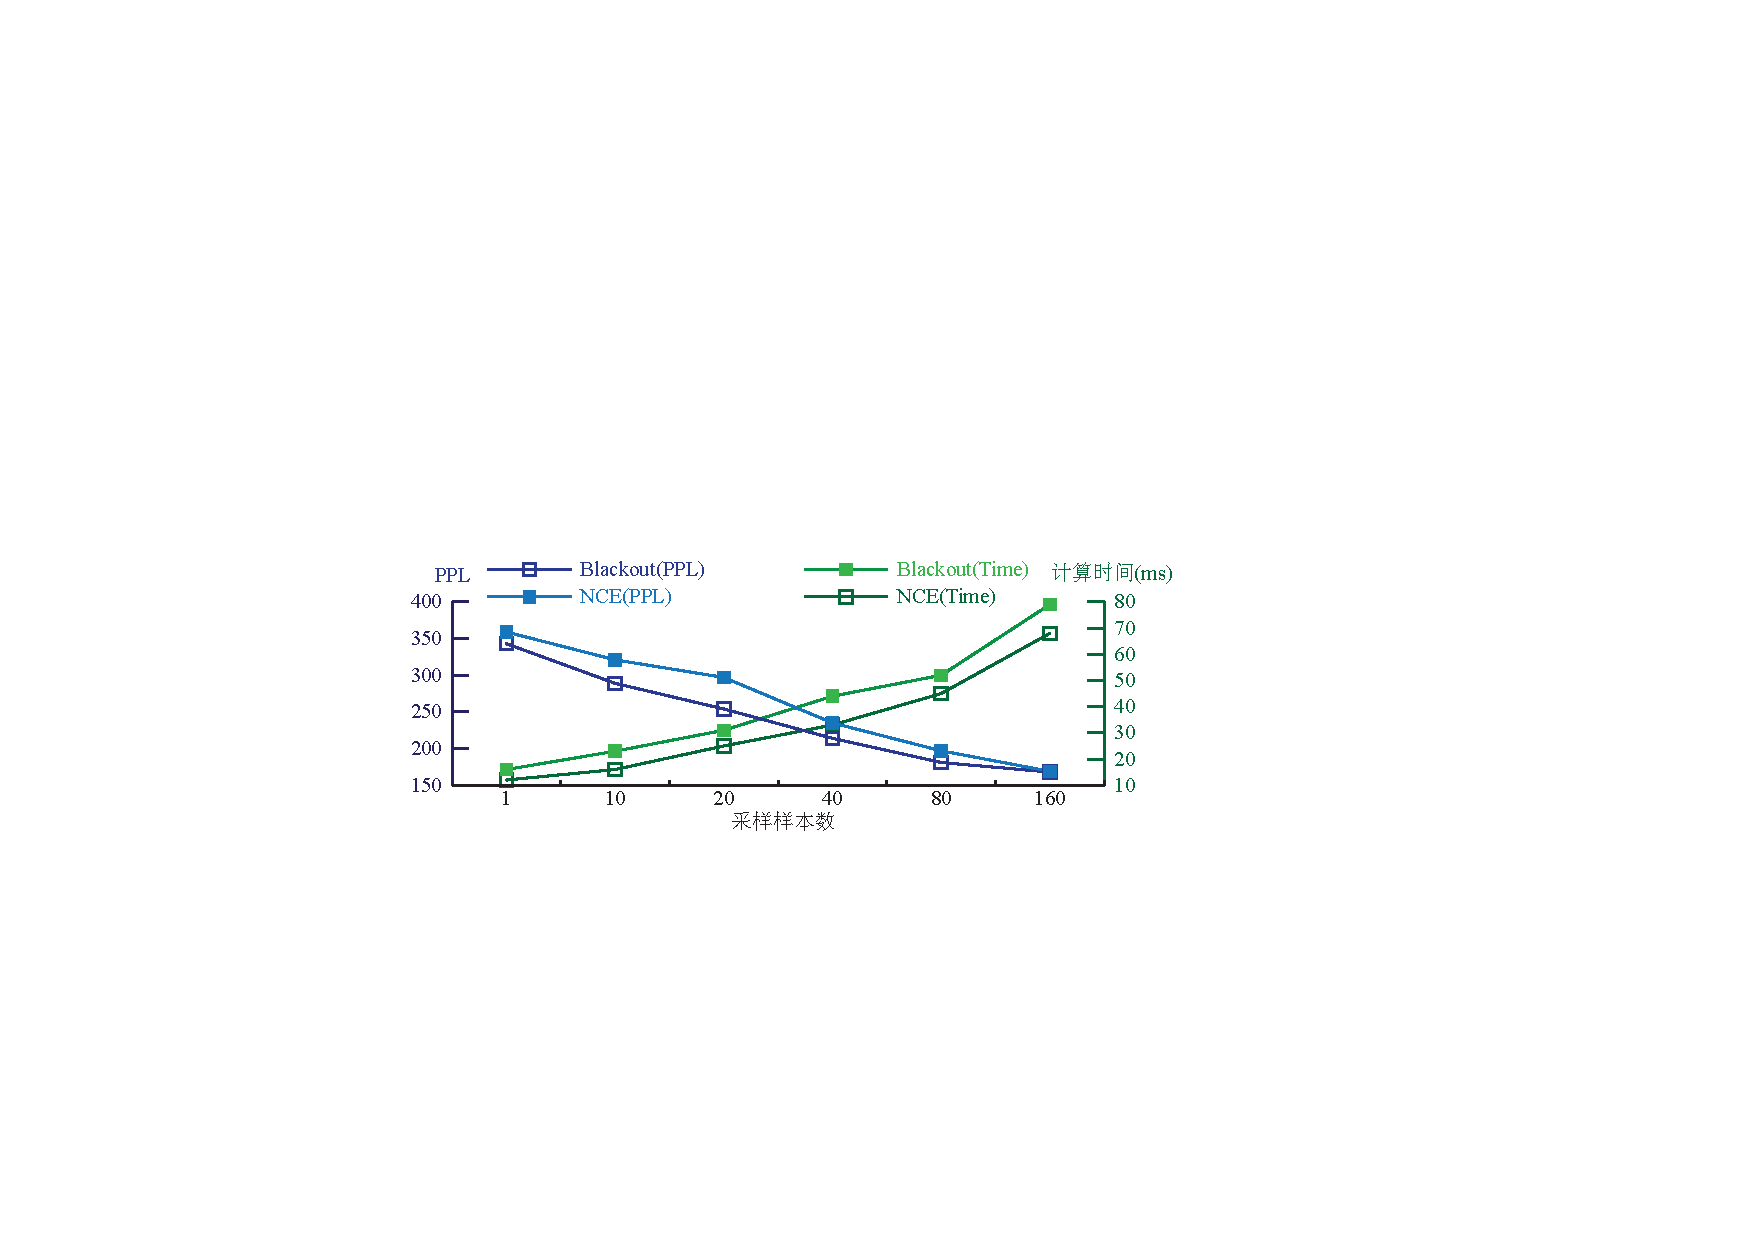
\includegraphics[width=.85\columnwidth]{./figures/nce_blackout.pdf}
  \caption{wikitext-2上测试不同采样数量对NCE和Blackout算法的影响}\label{fig:blackout_nce}
\end{figure}

我们发现一个样本大小和二元分类表现最差。训练过程涉及在真正的词概率阶段的学习,以及在噪声概率估计阶段的学习。因此,这些算法只能在收集足够的噪声样本时才能准确地估计噪声概率。这些估计算法的性能随着噪声样本数量的增加而收敛到最优混淆度,但加速比$ V / k $减小,其中$ k $表示样本大小。因此,我们把这个术语作为一个超参数,应该根据验证集进行调整,所以在训练过程中,每个特定数据集的样本量都是固定的。尽管如此,采样方法在推理过程中是不能使用的,而采用原始的softmax方法。



\subsection{单词聚类策略分析}
Chen~等人发现这个单词的层次聚类算法对cHSM算法的性能很敏感~\upcite{DBLP:conf/acl/ChenGA16}。同样,为了获得较为稳定的cHSM算法和p-HSM方法的性能,我们考虑了几个现有的聚类准则,如表~\ref{table:p-thsm}~和表~\ref{table:clustering}~所示。
\begin{table}[!t]
  \centering
   \caption{wikitext-2上评价不同聚类方法对p-HSM 算法的PPL影响\label{table:p-thsm}}
  \begin{tabular}{lcccc} \toprule
  算法  &建树时间&最大树深度 &验证集 (PPL) & 测试集 (PPL)  \\ \midrule
  Uigram  &3分钟&12 &218.42& 216.05     \\
  Bigram  &35小时&21& 186.23& 189.58\\
  Semantic &26小时 &18& \textbf{163.12} & \textbf{178.78}\\
\bottomrule
  \end{tabular}
\end{table}

\begin{table*}[!t]
  \centering
  \caption{wikitext-2数据集上不同聚类算法对cHSM 算法的PPL 和 WER 影响\label{table:clustering}}
  \begin{tabular}{lclccc} \toprule
聚类算法 & 均匀划分?&分支数& 训练轮数& 测试集 (PPL / WER)&耗时 (ms)\\ \midrule
  \multirow{6}{*}{Random}  &\multirow{6}{*}{是}&10/3330&145&211.15 / 78.55 &791\\
    &&20/1664&123&228.72 / 78.89&565\\
    &&40/832&103&234.36 / 79.21&321\\
    &&80/417&78&243.12 / 79.64&171\\
    &&160/208 &57&253.38 / 80.08&92\\
    &&182/183&48&268.63 / 80.11&88\\
  \midrule
  \multirow{6}{*}{Alphabet}  &\multirow{6}{*}{是}&10/3330 &141&199.01 / 78.07 &773\\
    &&20/1664 &120&211.34 / 78.23&551\\
    &&40/832 &100&238.75 / 79.02&313\\
    &&80/417 &90&241.75 / 79.34&174\\
    &&160/208 &56&248.35 / 79.62&97\\
    &&182/183&45&258.57 / 80.02&87\\
  \midrule
  \multirow{6}{*}{Uni-gram}   &\multirow{6}{*}{是} &10/3330&134&211.51 / 77.41 &788\\
    & &20/1664&122&220.01 / 77.71&549\\
    & &40/832&113&236.56 / 77.95&302\\
    & &80/417&91& 241.12 / 78.25&170\\
    & &160/208&55&247.25 / 79.21&93\\
    & &182/183&42&253.35 / 79.92&86\\
  \midrule
  \multirow{5}{*}{Bi-gram}   &\multirow{5}{*}{否}&10/3672&150&208.11 / 77.32&801\\
     &&20/1923&121&217,34 / 77.64&621\\
     &&40/1123&102&228.87 / 78.14&588\\
     &&80/572&89&246.32 / 78.43&186\\
     &&160/340&76&252.33 / 79.51&97\\
  \midrule
  \multirow{5}{*}{Syntactic}  &\multirow{5}{*}{否}&10/3612 &152&214.31 / 78.11&810\\
    &&20/1972 &130&220.19 / 78.86&633\\
    &&40/996 &101&232.33 / 79.33&543\\
    &&80/545 &89&241.34 / 79.84&179\\
    &&160/235 &70&262.34 / 80.14&134\\
  \midrule
  \multirow{5}{*}{Semantic}  &\multirow{5}{*}{否} &10/3570 &133&208.77 / 77.41&819\\
    & &20/1873 &114&218.31 / 77.78&641\\
    & &40/1092 &91&225.38 / 78.35&521\\
    & &80/561 &69&238.45 / 78.91&174\\
    & &160/244 &44&256.75 / 79.41&103\\
\bottomrule
  \end{tabular}
\end{table*}

一方面,我们将表~\ref{table:clustering}中的Wikitext-2数据集中,应用前面所有提到的聚类方法,同时比较了不同的分支因子对算法效果的影响,并进行了比较。从这张表中可以发现,随机洗牌方法对于其他算法的性能最差,因为它们没有提供有关先前分配的任何信息。此外,还观察到,比其他人更难以接受可接受的训练损失,因此在训练集上花费更多的时间来优化参数。然后,发现在对类结构注入外部单字和双字的知识之后,模型确实在目标空间中学习了一个明确定义的单词分布。因此,它对随机和字母表系列取得了更好的结果。而且,用语法和语义算法进行分词的词汇比上述方法得到的结果要好得多,代价是计算分割方法。从实验结果可以看出,向具有先验知识的类结构注入会增强该方法的稳定性,通过平衡聚类时间和模型的准确性,可以调整分支因子,达到预期的结果。



另一方面,我们采用了单词,字母和词汇聚类方法来生成单词在树上的分布,详细的结果在表~\ref{table:clustering}~中给出。与提供调整分支因子的自由度的cHSM方法不同,树聚类的实验是相当有限的。单字聚类(即频率合并)方法在创建单词层次结构方面效率更高,而双字词和语义聚类花费更多时间来计算词汇表中单词之间的相似度矩阵。尽管如此,考虑到树合并的规则,bigram方法考虑了二元共现统计和语义方法来评估特征空间中的欧氏距离。在困惑度量下,二元语义聚类方法比一元方法有更好的效果。最后,与cHSM方法相比,更深层次的树模型更适合于词汇聚类,适当的聚类可以提高树层次的效率。

\section{模型总体评价}
如表~\ref{tab:summary_ppl}~所示,我们收集了上述三种标准语料库的验证和测试数据集的所有困惑和错误率结果。值得注意的是,我们采用了一层GRU单元作为所有这些算法的上下文表示,其维数设置为256.另外,对于NCE和Blackout近似,超参数$ k $是 对较小的Wikitext-2和Wikitext-103数据集设置为$\mathcal{|V|}/20 $,对于较大的One Billion Word数据集,设置为$ k = | \mathcal{V} | / 200 $。 此外,对于cHSM方法,我们根据单词的单字分布来划分词汇。

考虑到Wikitext-2数据集上的结果,最初的softmax比其他算法获得了最好的分数,因为在Blackout和NCE近似中没有引入任何cHSM和p-tHSM算法的结构损失或基于抽样的变分损失。

\begin{table}[!h]
  \centering
  \caption{所有模型在三个数据集上的困惑度和单词错误率的性能评测\label{tab:summary_ppl}}
\begin{tabular}{llcc}
  \toprule
数据集& 算法& 验证集(PPL/WER) & 测试集(PPL/WER) \\ \midrule
 \multirow{2}{*}{WikiText-2}&GRU + Softmax&172.64 / 77.49\%&162.09 / 77.07\% \\
  &GRU + NCE~\upcite{DBLP:journals/jmlr/GutmannH10}&217.84 / 78.26\%&199.54 / 78.02\%\\
  &GRU + Blackout~\upcite{DBLP:journals/iclr/JiVSAD15}&221.15 / 77.72\%&199.56 / 77.50\% \\
  &GRU + cHSM + unigram~\upcite{DBLP:conf/acl/ChenGA16}&253.18 / 78.25\%&236.61 / 78.02\%\\
  &GRU + p-tHSM + unigram~\upcite{DBLP:conf/nips/MikolovSCCD13}&218.42 / 78.15\%&216.05 / 78.15\%\\
  &GRU + p-tHSM + bigram~\upcite{DBLP:journals/coling/BrownPdLM92}&186.23 / 78.15\%&189.58 / 78.15\%\\\midrule
   \multirow{2}{*}{WikiText-103} &GRU + Softmax&130.38 / 72.15\%&136.83 / 72.37\%\\
 &GRU + NCE~\upcite{DBLP:journals/jmlr/GutmannH10}&164.78 / 73.22\%&165.01 / 73.34\%\\
  &GRU + Blackout~\upcite{DBLP:journals/iclr/JiVSAD15}&163.99 / 73.18\%&162.76 / 74.22\%\\
  &GRU + cHSM + unigram~\upcite{DBLP:conf/acl/ChenGA16}&171.81 / 73.42\%&166.74 / 73.18\%\\
  &GRU + p-tHSM + unigram~\upcite{DBLP:conf/nips/MikolovSCCD13}&165.70 / 73.53\%&166.11 / 72.44\%\\
  &GRU + p-tHSM + bigram~\upcite{DBLP:journals/coling/BrownPdLM92}&164.15 / 78.15\%&163.55 / 77.85\%\\\midrule
  \multirow{2}{*}{One Billion Word} &GRU + Softmax&330.38 / 88.15\%&330.83 / 88.37\%\\
 & GRU + NCE~\upcite{DBLP:journals/jmlr/GutmannH10}&272.07 / 84.83\%&276.11 / 84.34\%\\
  &GRU + Blackout~\upcite{DBLP:journals/iclr/JiVSAD15}&268.67 / 84.23\%&266.11 / 84.18\%\\
 & GRU + cHSM + unigram~\upcite{DBLP:conf/acl/ChenGA16}&225.36 / 80.32\%&224.11 / 79.42\%\\
 & GRU + p-tHSM + unigram~\upcite{DBLP:conf/nips/MikolovSCCD13}&231.44 / 87.53\%&236.11 / 82.53\%\\
  &GRU + p-tHSM + bigram~\upcite{DBLP:journals/coling/BrownPdLM92}& 221.55 / 81.15\%&218.70 / 83.15\%\\
  \bottomrule
\end{tabular}
\end{table}

对于第二个Wikitext-103数据集,Brown聚类的p-tHSM方法不仅获得了比霍夫曼聚类方法更好的结果,而且表现也比其他方法好。另外,cHSM模型能够获得与p-tHSM变体类似的结果,表明我们可以用其他合适的用于cHSM方法的聚类算法获得更好的结果。由于Wikitext-103和Wikitext-2数据集共享相同的测试集,因此发现最初的softmax通过更大的训练数据被收敛到更好的结果。此外,对于采样方法,它收敛于比softmax方法好得多的结果,同时提高了时间效率。

综上所述,在用字极性编码方案替代tHSM中的传统霍夫曼编码方案并且实现了基于紧密的树型模型p-tHSM之后,我们证明了这种新颖的编码方案允许在GPU上并行运行计算。这将原始tHSM的时间复杂度从$ \mathcal {O(| H | \log | V |)} $减少到$\mathcal{O(| H || V |)} $并获得了最佳的加速比对于大量的词汇问题。此外,为了稳定p-tHSM模型的性能,我们测试了几种现有的层次聚类算法,发现基于树模型的词聚类与内部节点的二元分类密切相关。

\section{本章小结}

词汇量过大问题是语言模型应用中最重要的挑战之一。为了解决这个问题,文献中提出了各种方法,可大致分为三个类别:词汇截断算法,基于抽样的近似算法和词表层次分解。第一种方法易于实施,并广泛应用于实践中。而第二类可以有效地减少训练时间消耗,而不用通过重要性抽样的变化来总结所有的单词,而抽样分布的选择可以针对更稳定的结果进行优化。第三种方法将目标词汇的扁平化架构改变为具有两种可能类型的启发式分层结构:类和树因式分解。构建在两步softmax分类方法和树模型上的类方法将其扩展到$\mathcal {O(| H | \log | V |)} $步骤的二进制分类。

在这个研究中,我们不仅提出了基于二叉树或者分类层次概率模型的潜在编码方案,而且为分层softmax变体建立了并行和紧凑的损失函数。另外,利用GPU硬件的优势,可以有效地计算出目标词汇量越来越大的概率和梯度。值得注意的是,这个算法的时间复杂度超出了历史记录$ \mathcal {O(| H | \log | V |)}$,从而使它能够处理大量的词汇问题。此外,我们还扩展了几个推理策略来进行评分或排名。在实验中提出并讨论了三种算法,在分析部分中进行了很好的说明。最后,我们评估了几个单词层次聚类算法,以更有效的方式组织树中的单词。结果表明,与其他概率归一化方法相比,加速比提高,得到更高效的树聚类,与其他基于抽样的优化相比,性能相对较好。

在未来的研究中,我们计划探索softplus函数的应用场景,并探讨在cHSM算法训练的时候的词表动态交换算法。另外,实验中应用的几种聚类算法消耗了很多时间,我们可以优化该聚类算法,设计更高效的分层结构。

\summary
大词表问题是语言模型应用中最重要的挑战之一,为了解决这个问题,文献中提出了各种方法可大致分为三个类别:词汇截断算法,基于抽样的近似算法和词表层次分解。第三种方法将目标词汇的扁平化架构改变为具有两种可能的分层结构:类和树层次分解。构建在两步softmax分类方法和树模型上的类方法将其扩展到$\mathcal {O(| H | \log | V |)} $步骤的二进制分类。Mikolov~曾提出使用基于二叉树的层级概率模型来加速的训练方案,加速比能达到理论的最大速度,但是当时提出的背景是基于CPU构建的,如今越来越多的算法随着应用领域的推广,需要在并行度更高的~GPGPU~设备上进行计算,因此基于GPGPU进行建模的层次概率模型尚未被研究提及,需要在本文中研讨。
\section*{工作总结}
当我们使用多层分类模型的时候,我们就需要将单词按照模型的架构进行划分。其中对于cHSM模型,我们有以下策略可以使用:基于词频划分类别、 基于布朗聚类进行划分、按照词向量信息进行聚类等方法。另外,我们还需要注意的是,词表可以均匀划分,也可以非均匀划分,与具体层次聚类算法相关。


\noindent 1. 本论文中,针对两种层次概率模型,首先定义了对应编码方式,同时给出了模型所涉及的参数的详细含义。接下来,我们逐步推导模型的单个节点的概率公式,单个词的概率公式和模型的代价函数。另一方面,我们将提出的~p-tHSM~算法和传统的线性~tHSM~算法进行的比较。通过比较两者计算的差异性证明我们提出的算法更适合在GPGPU等高并行设备上运算。进一步的,我们还讨论了模型在测试的时候所需的推理算法,因为基于层次结构的概率计算方案和传统的softmax计算方案不同,不能直接输出单个词的概率或者计算最佳的候选单词,所以我们分别针对这两个任务提出推理算法。最后,由于单词在二叉树上的分布需要初始化,我们讨论了现存的各种聚类算法效果。

\noindent 2. 在实际实验中,我们提出的层次概率模型的时间复杂度超出了$\mathcal{O(|H|\log|V|)}$的历史记录,从而证明它能够处理大量的词汇问题。此外,我们基于模型的排序打分两个实验,验证了我们提出的测试阶段需要应用的推理算法。。最后,我们评估了几个单词层次聚类算法,以更有效的方式组织树中的单词。结果表明,与其他概率归一化方法相比,加速比提高,得到更高效的树聚类,与其他基于抽样的优化相比,性能相对较好。

\section*{工作展望}
本文提出的层次概率模型在语言模型的各项评测上取得了有效的结果,验证了本方法的合理性。但是该方法还存在进一步提升的空间:

\noindent 1. 大规模实验数据分析验证算法:由于在现有实验环境条件下,在大数据集上的实验验过程收敛很慢,所以目前的实验主要还是在小规模数据集上进行了初步验证,下一步将进一步在大数据集上进行验证并比较算法的差异,进一步验证算法的广泛适用性。

\noindent 2. 由于我们选择的建模平台是python平台,好处是可以使用许多现成的已有的框架。并且python语法简单,矩阵计算库numpy和scipy更成熟,便于调试。另一方面,我们采用的建模语言是theano框架,它的底层计算都是调用BLAS计算库,或者直接调用基于GPGPU的CUDA的CuBLAS计算库。虽然这样做便于在前期模型建立阶段能方便尝试各种设计方案,但是他的计算瓶颈在python解释器对代码的缓慢执行,所以如果能将部分模型组件使用CUDA语言重写,使得本论文提出的模型能接受一定的组合排列的可能性,将使得整体计算速度能得到更大提升,这也是许多目前流行框架发展的方向,例如Mxnet\footnote{http://mxnet.incubator.apache.org/}直接使用C++ 语言建立深度模型,他的计算效率也是目前已知的框架中最快的。因此,考虑到目前的Thenao计算瓶颈,下一步将重点研究如何将RNN的框架使用CUDA语言重构,并基于CuDNN 库开发的样板进行改进。


\noindent 3. 本实验中采用了不同聚类算法,并分析了各个聚类算法的优劣。目前采用的聚类算法计算非常费时,尤其是当我们希望进行多层次聚类的时候,我们需要花费数周时间来获得结果。这样的缓慢的计算效果是无法接受的,经过针对代码的调试,我们发现计算瓶颈在算法初始化的时候,计算两两单词之间的距离,它花费了90\%的计算时间。如果能存在有效的初始化算法,而不是挑选尽可能高精度的聚类模型,那么实验进度和试验结果就可以针对多组参数调试。我们也可以考虑,单词分布也是随机初始化,在模型训练的时候动态计算单词交换策略,随着模型的收敛,单词的划分也逐渐收敛,这样一来我们就不需要在使用额外的计算库,给我们的模型添加各种数据。除此之外,我们还需要探讨除了语言模型一种应用场景,我们还可以应用到大规模标签分类,或者更接近的机器翻译领域中。


% 参考文献
\cleardoublepage
\phantomsection
\addcontentsline{toc}{chapter}{参考文献}
\nocite{*}
\bibliographystyle{GBT7714-2005}%ZJUthesis}
\bibliography{thesis_reference}
\cleardoublepage

% 附录
%\appendix

% 附页标题样式
\backmatter
% 附页\emph{}
\chapter{攻读硕士学位期间取得的学术成果}
% 此处标题及内容请自行更改
\noindent 发表论文:
\begin{enumerate}[label=\arabic*.]
\item \textbf{Nan Jiang}, Wenge Rong, Min Gao, Yikang Shen and Zhang Xiong. Exploration of Treebased Hierarchical Softmax for Recurrent Language Models[A]. Proceedings of the 26th International Joint Conference on Artificial Intelligence[C]. 2017: 1951-1957.
\item \textbf{Nan Jiang}, Wenge Rong, Yifan Nie, Yikang Shen and Zhang Xiong. Event Trigger Identification with Noise Contrastive Estimation[J]. IEEE/ACM Transactions on Computational Biology and Bioinformatics, 2017. (Accepted)
\item \textbf{Nan Jiang}, Wenge Rong, Baolin Peng, Yifan Nie and Zhang Xiong. Modeling Joint Representation with Tri-Modal DBNs for Query and Question Matching[J]. IEICE Transactions on Information and Systems, 2016, 99(4): 927-935.
\item \textbf{Nan Jiang}, Wenge Rong, Baolin Peng, Yifan Nie and Zhang Xiong. An Empirical Analysis of Different Sparse Penalties for Autoencoder in Unsupervised Feature Learning[A]. Proceedings of 2015 International Joint Conference on Neural Networks[C]. 2015: 1-8.
\end{enumerate}
\noindent 投稿论文:
\begin{enumerate}[label=\arabic*]
\item \textbf{Nan Jiang}, Wenge Rong, Min Gao, Yikang Shen and Zhang Xiong. Exploration of Hierarchical Softmax for Recurrent Language Models[J]. ACM Transactions on Intelligent Systems and Technology. (Submitted)
\end{enumerate}
\chapter{致\quad 谢}
在2015年,我来到了北航计算机学院工程研究中心,开始了我研究生学习阶段。首先感谢荣文戈副教授当年的知遇之恩,没有导师指点与意见,我也不会成为现在的我。同时,更想感谢熊璋老师、欧阳元新老师和王静远老师,他们对我的谆谆教导,是我在遇到苦难的时候能够不言放弃,努力解决问题所在。

我能够顺利完成研究生阶段的求学,离不开荣老师的悉心指导和耐心改正我的错误。荣老师不仅为我设定了远大的目标,还真且关注我的水平的成长,每次都是设置一个能力可及的任务,不断锻炼我的写作技能和实验技能。最令人记忆深刻的是,在每次论文投稿前一周,每当深夜我将论文修订完一版本之后,荣老师总是立马修改,甚至在早上四点给我修改论文。顶着巨大的身体压力和时间压力,给我不断修改论文,还不断跟我捋顺论文思路,其耐心已经超越了我人生认识的所有老师。然而学术的生涯并不总是一帆风顺的,在很长一段时间的瓶颈期,荣老师在听完我不断的抱怨之后,仍然鼓励我,帮我树立做科研的自信心,使我明白不断加强自身知识和技术水平的重要性。经过整整大半年的低谷时期,总算迎来了一点新的成果,此时的我非常膨胀,自视甚高。此时荣老师又劝导我,过度自信和过度自我否定都是不可取的,人生路尚且长,我们需要走好每一步,不要因为别人的质疑而否定自己,更不能因为别人的赞美而吹嘘自己。

%自小离家求学,父母的管教未曾领受,导致现在的我存在诸多性格和学习态度上的缺点,荣老师在这两年里,如醍醐灌顶一般,将他的人生哲学授予我,实在是不可多得的财富。相比于那些物质上的利益,导师传授的这些哲学才是颠扑不破的道理。

还要感谢实验室的学长和学弟对我的呵护和指点。其中包括:陈虞君博士、张硕师姐、聂一凡大师兄、沈驿康师兄。还有已经毕业的宋欣、谢维柱师兄。令人记忆深刻的是我当初投稿阶段,实验需要很多台计算设备,他们听到我的需求,帮助我在他们的高精度计算平台上开展实验工作。除此之外,我还要感谢可爱的师弟师妹们,是黎彬、田川师弟。还要感谢邱晨和高志峰提供源源不断有关实验和算法的建议。

最后感谢我的父母,由于家境不是很好,父母从我三岁开始去上海打工,历时20余载,一直坚守在自己的岗位上,为了我的以后的未来,积攒下一点积蓄。尽管他们远在他乡,对我的学业也是非常的关心,每周都得电话通讯,报告进期的教授的知识和学业成绩。没有一句累了不想干了,我因有他们一直陪在我身边感到幸运,因他们的不懈付出而感到学业有成的重要性。

\end{document}
